\section{The Two Primary Accumulation Points}
This section will provide a visual overview of the results concerning the two primary sequences of special parameter values as we approach $s_1^l$ from the right and $\pr$ from the left. The following propositions from Chapter 4 summarize the accumulation that we are seeing in the figures to follow:

\begin{customthm}{\ref{homaccum}}
% On the interval $ (\pl, \pr)$, there is an accumulation of parameter values $p_n^{CrF^{n-2}C}$ and $z_n^{CrF^{n-2}0}$ for any integer $n \geq 2$ such that 
% \[
% z_n^{CrF^{n-2}0} < p_n^{CrF^{n-2}C} < z_{n+1}^{CrF^{n-1}0} < p_{n+1}^{CrF^{n-1}C}
% \]
% The numerics suggest that the accumulation will limit to the point $P_c$.
On the interval $ (\pl, \pr)$, there is an accumulation of parameter values $p_n$ and $z_n$ for any integer $n \geq 2$ where the critical orbit has coding $CrF^{n-2}C$ and $CrF^{n-2}0$ respectively. These parameter values have the ordering
\[
z_n < p_n < z_{n+1} < p_{n+1} < \cdots < h_2^{CrP_c}
\]
\end{customthm}

\begin{customthm}{\ref{sadaccum}}
% On the interval $ (\pl, \pr)$, there is an accumulation of parameter values $p_n^{Cr^{n-1}C}$, $z_n^{Cr^{n-1}0}$, and $h_n^{Cr^{n-1}P_c}$ for any integer $n \geq 2$ such that 
% \[
% z_{n+1}^{Cr^{n}0} < p_{n+1}^{Cr^{n}C} < h_{n+1}^{Cr^{n}P_c} < z_n^{Cr^{n-1}0} < p_n^{Cr^{n-1}C}  < h_n^{Cr^{n-1}P_c}
% \]
% The numerics suggest that the accumulation will limit to the point $s^l_1$.
On the interval $ (\pl, \pr)$, there is an accumulation of parameter values $p_n$, $z_n$, and $h_n$ for any integer $n \geq 2$ where the critical orbit has coding $Cr^{n-1}C$, $Cr^{n-1}0$, and $Cr^{n-1}P_c$ respectively. These parameter values have the ordering
\[
p_1^{-C} < \cdots < z_{n+1} < p_{n+1} < h_{n+1} < z_n < p_n < h_n
\]
\end{customthm}

Chapter 4 will introduce the proofs of these propositions; the remainder of this section is devoted to developing some graphical intuition as to how these accumulations propagate. Additionally these figures will serve as a useful reference when reading the proofs of the following chapter.  First, Figure \ref{hqorb} shows a large zoom of the Orbit Diagram for the parameter interval $ (\pl, \pr)$. Labeled on this figure are several of the $p_n$ values described in the above propositions with their coding. Based on a glance of this image, there seems to be some sort of limiting behavior as we approach either side of the parameter interval.

Next, Figure \ref{hqcplot} shows a plot of $f_c^1 (C)$, $f_c^2 (C)$, and $f_c^3 (C)$ where we are varying our parameter $c$ and looking at how each iterate of the critical point is changing (note that this plot is in the same space as the Orbit Diagram). On this plot we again show the coding intervals and label several of the accumulating parameter values as we approach $\pl$ from the right and $\pr$ from the left. Hopefully this image provides some sense as to where the special parameter values come from: in this space, they are simply the parameter values of intersections of some iterate of the critical point with some special value 0, $C$, or $P_c$, yielding a $z_n$, $p_n$, or $h_n$ respectively.

Figures \ref{fig:giters} and \ref{fig:giters2} provide graphical iteration of the right hand critical point at many of the key parameter values discussed so far. These figures are especially illuminating when considered as a sequence of images as $c$ decreases because one can gain an intuition as to how the system is evolving: as $c$ decreases from $\pr$, the second iterate moves down the curve from $P_c$ and in so doing, lands on several points which either cycle back to $C$ (giving a $p_n$), eventually land on 0 (giving a $z_n$), or eventually land on $P_c$ (giving an $h_n$). Again the codings of critical orbit at these parameter values can be constructed by following the graphical iteration.

Figure \ref{fig:iterh1} shows a sequence of images which depict the accumulation of $p_n$ and $z_n$ parameter values as we approach $\pr$. This sequence of images is a particularly good way to look at the accumulation because it is a visualization of the inductive proof of Proposition \ref{homaccum}. For any $n \geq 2$, $f^n_{\pr} (C) = P_c$ simply because the second iterate is fixed there (fixing all higher iterates). Then as we add higher iterates, we see that $f^{n+1}_{p_n} (C) < 0$, meaning that as the $n^{th}$ iterate makes its way to $P_c$ at $\pr$, it must cross the value $C$, giving a $p_n$, forcing the next iterate to be negative. In this manner, the proof of Proposition \ref{homaccum} constructs the sequence of $p_n$ and $z_n$ parameter values as required.

In a similar manner to Figure \ref{fig:iterh1}, Figure \ref{fig:iterh2} shows a sequence of images which depict the accumulation of $p_n$, $z_n$, and $h_n$ parameter values as we approach $\pl$. Again this is a great visualization of the proof of Proposition \ref{sadaccum}. For any $n \geq 1$, $f^n_{p_1^{-C}} (C) = -C$ simply because the first iterate is fixed there (fixing all higher iterates). Then as we add higher iterates, we see that $f^{n+1}_{z_n} (C) = \infty$, meaning that as the $n^{th}$ iterate makes its way to $-C$ at $p_1^{-C}$, it must cross the value $0$, giving a $p_n, h_n$, and then finally a $z_n$, forcing the next iterate to be $\infty$. This iterate must also make its way down to $-C$ so continuing in this manner, the proof of Proposition \ref{sadaccum} constructs the sequence of $p_n$, $h_n$, and $z_n$ parameter values as required.
\begin{sidewaysfigure}[ht]
	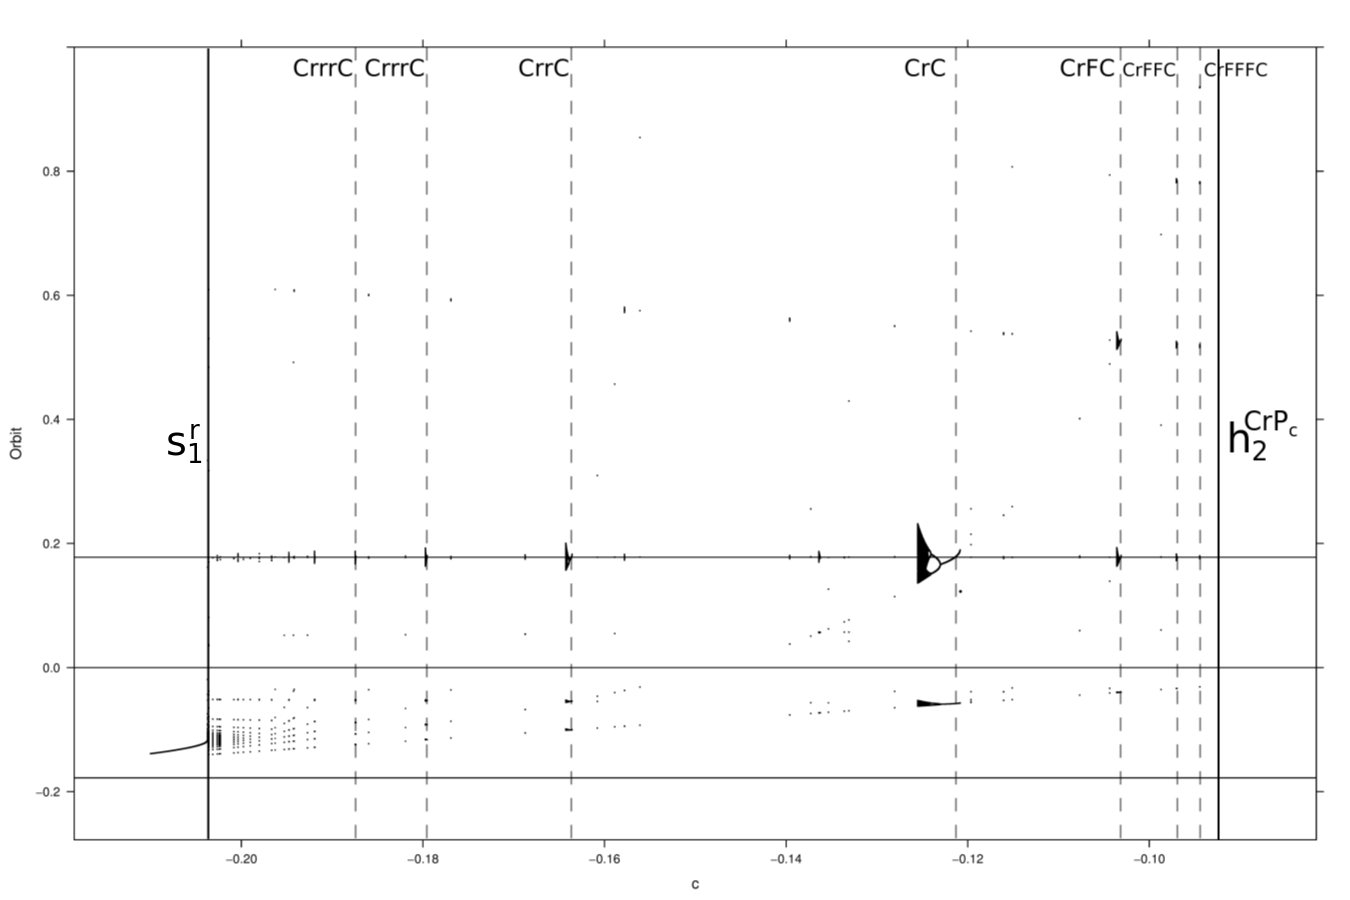
\includegraphics[width=\textheight]{./img/over.png}
	\caption{A high quality orbit diagram with several $p_n$ values and their codings indicated}
	\label{hqorb}
\end{sidewaysfigure}

\begin{sidewaysfigure}[ht]
	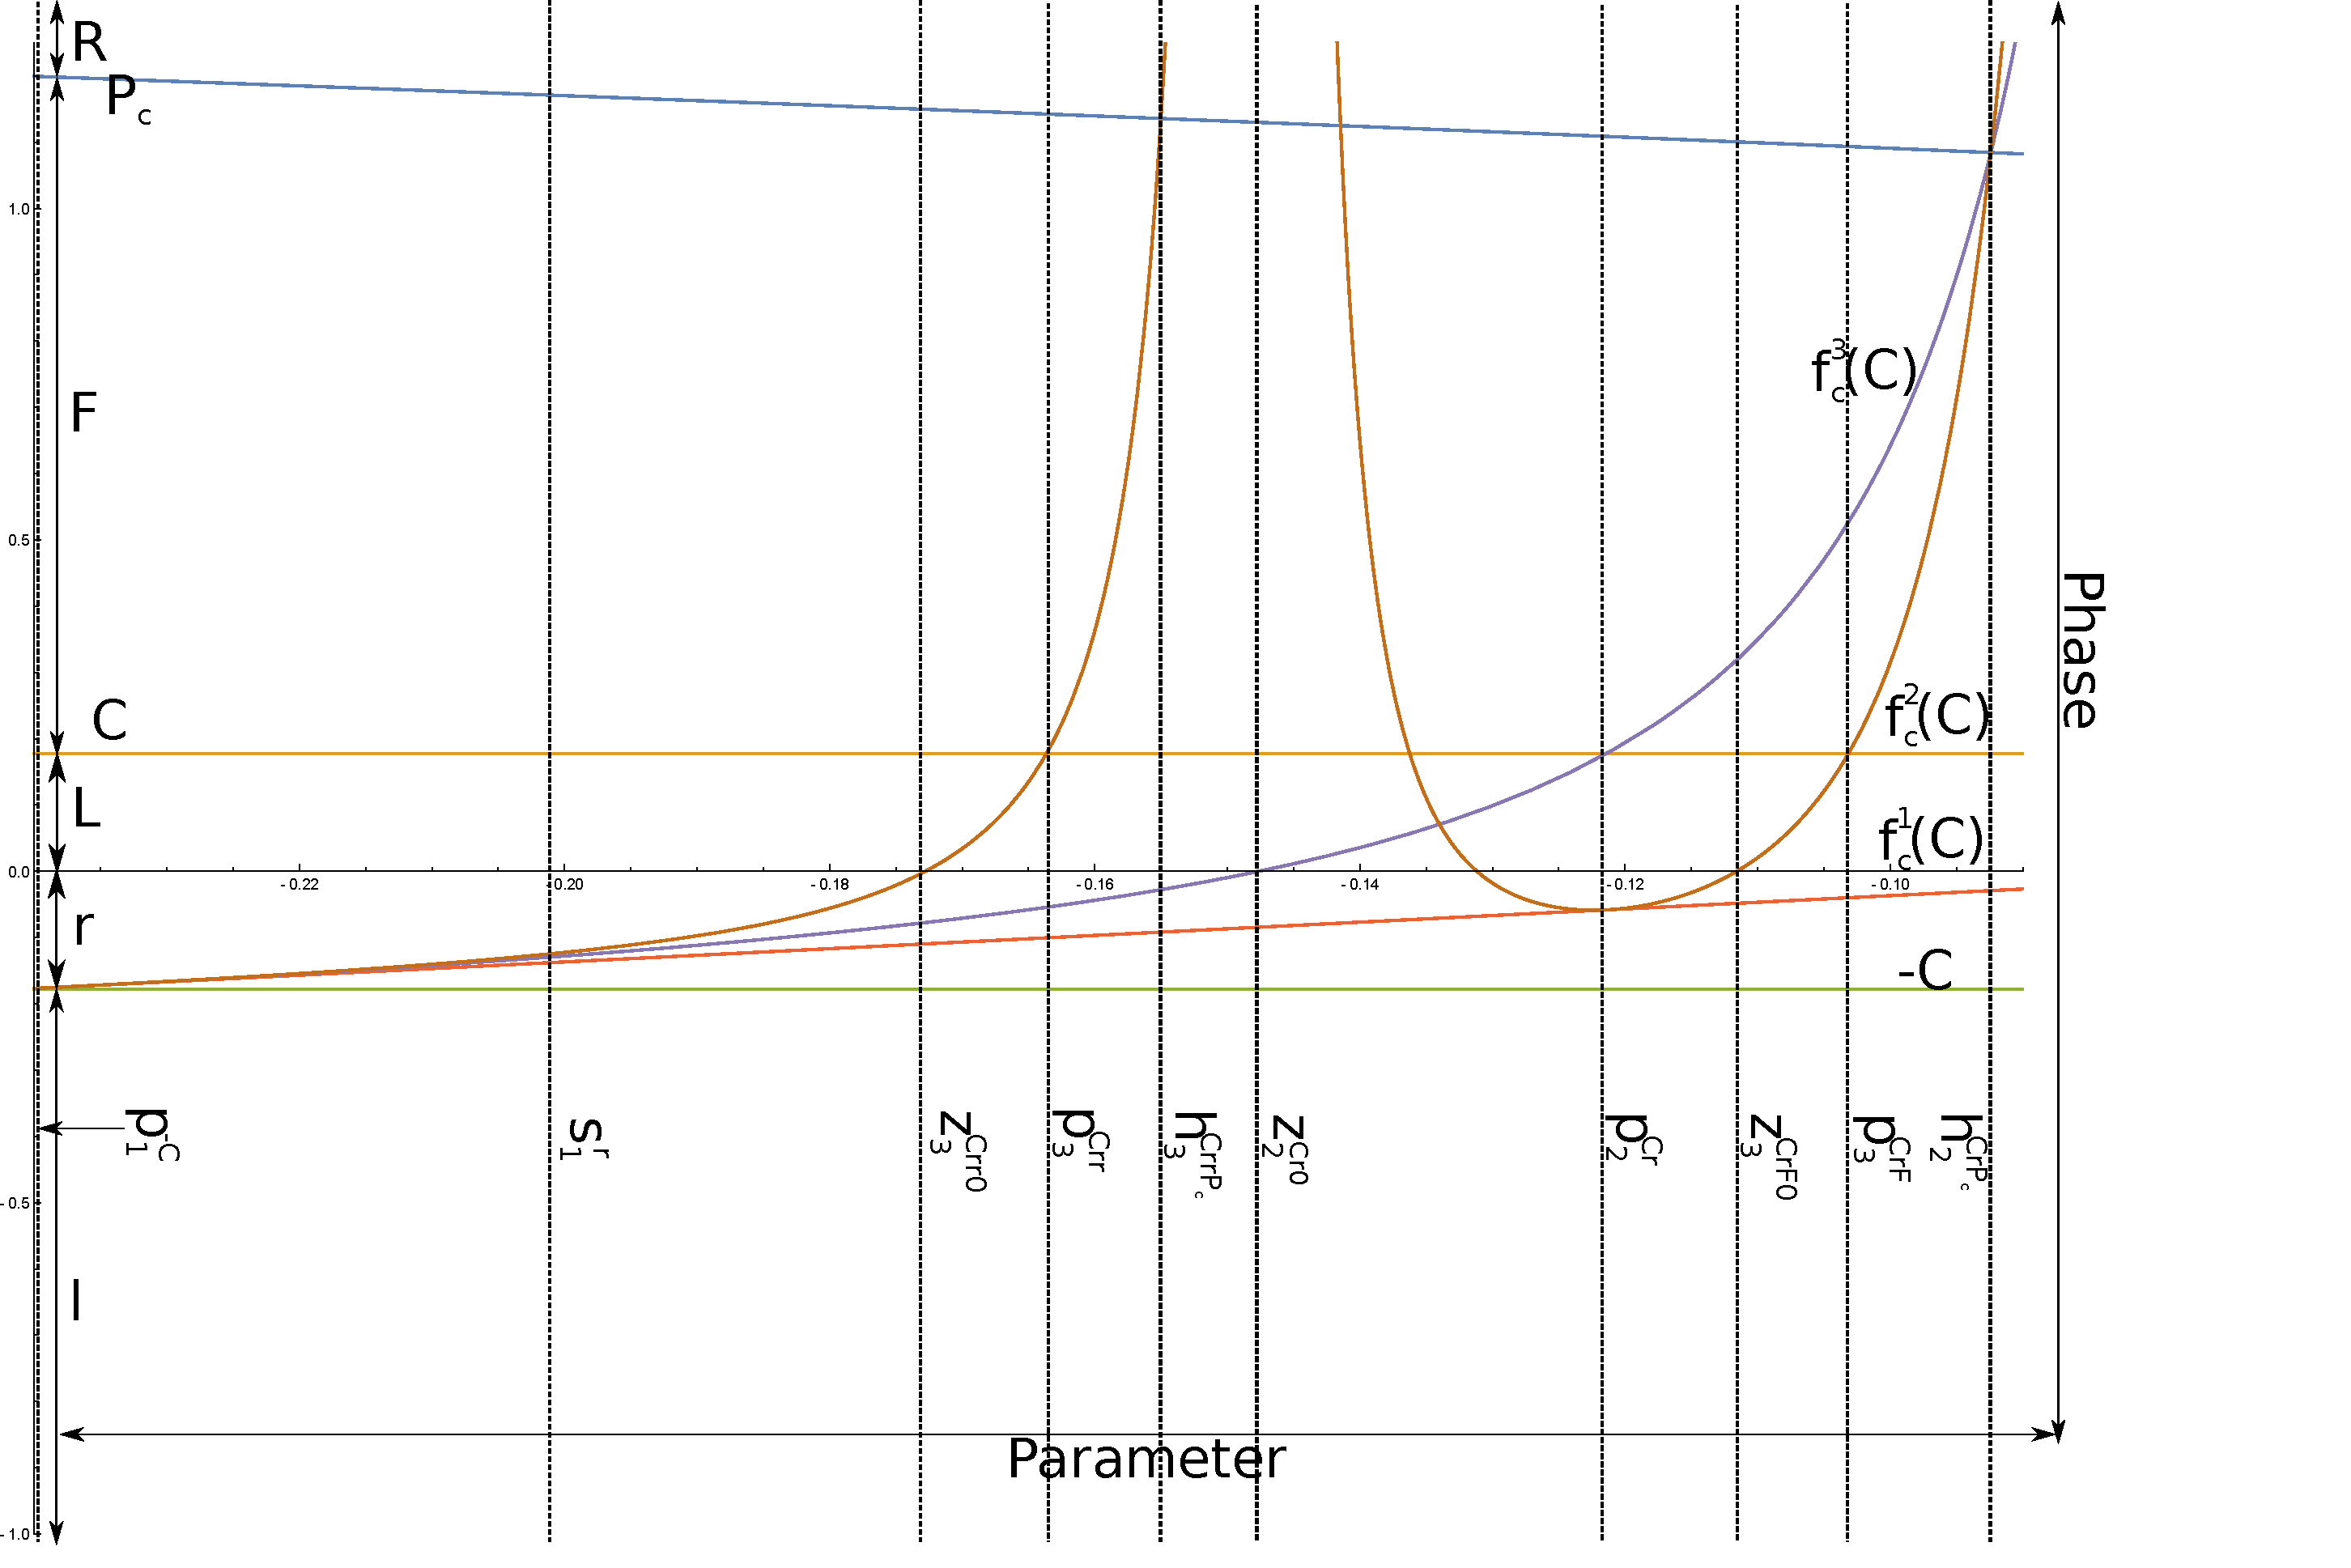
\includegraphics[width=\textheight]{./img/cs2}
	\caption{A plot of $f^1_c (C),f^2_c (C),f^3_c (C)$ in parameter$\times$phase space with the ``primary'' parameters labeled for $h_n,p_n,z_n$}
	\label{hqcplot}
\end{sidewaysfigure}

\begin{figure}[ht]
		\centering
		\begin{subfigure}[b]{0.3\textwidth}
				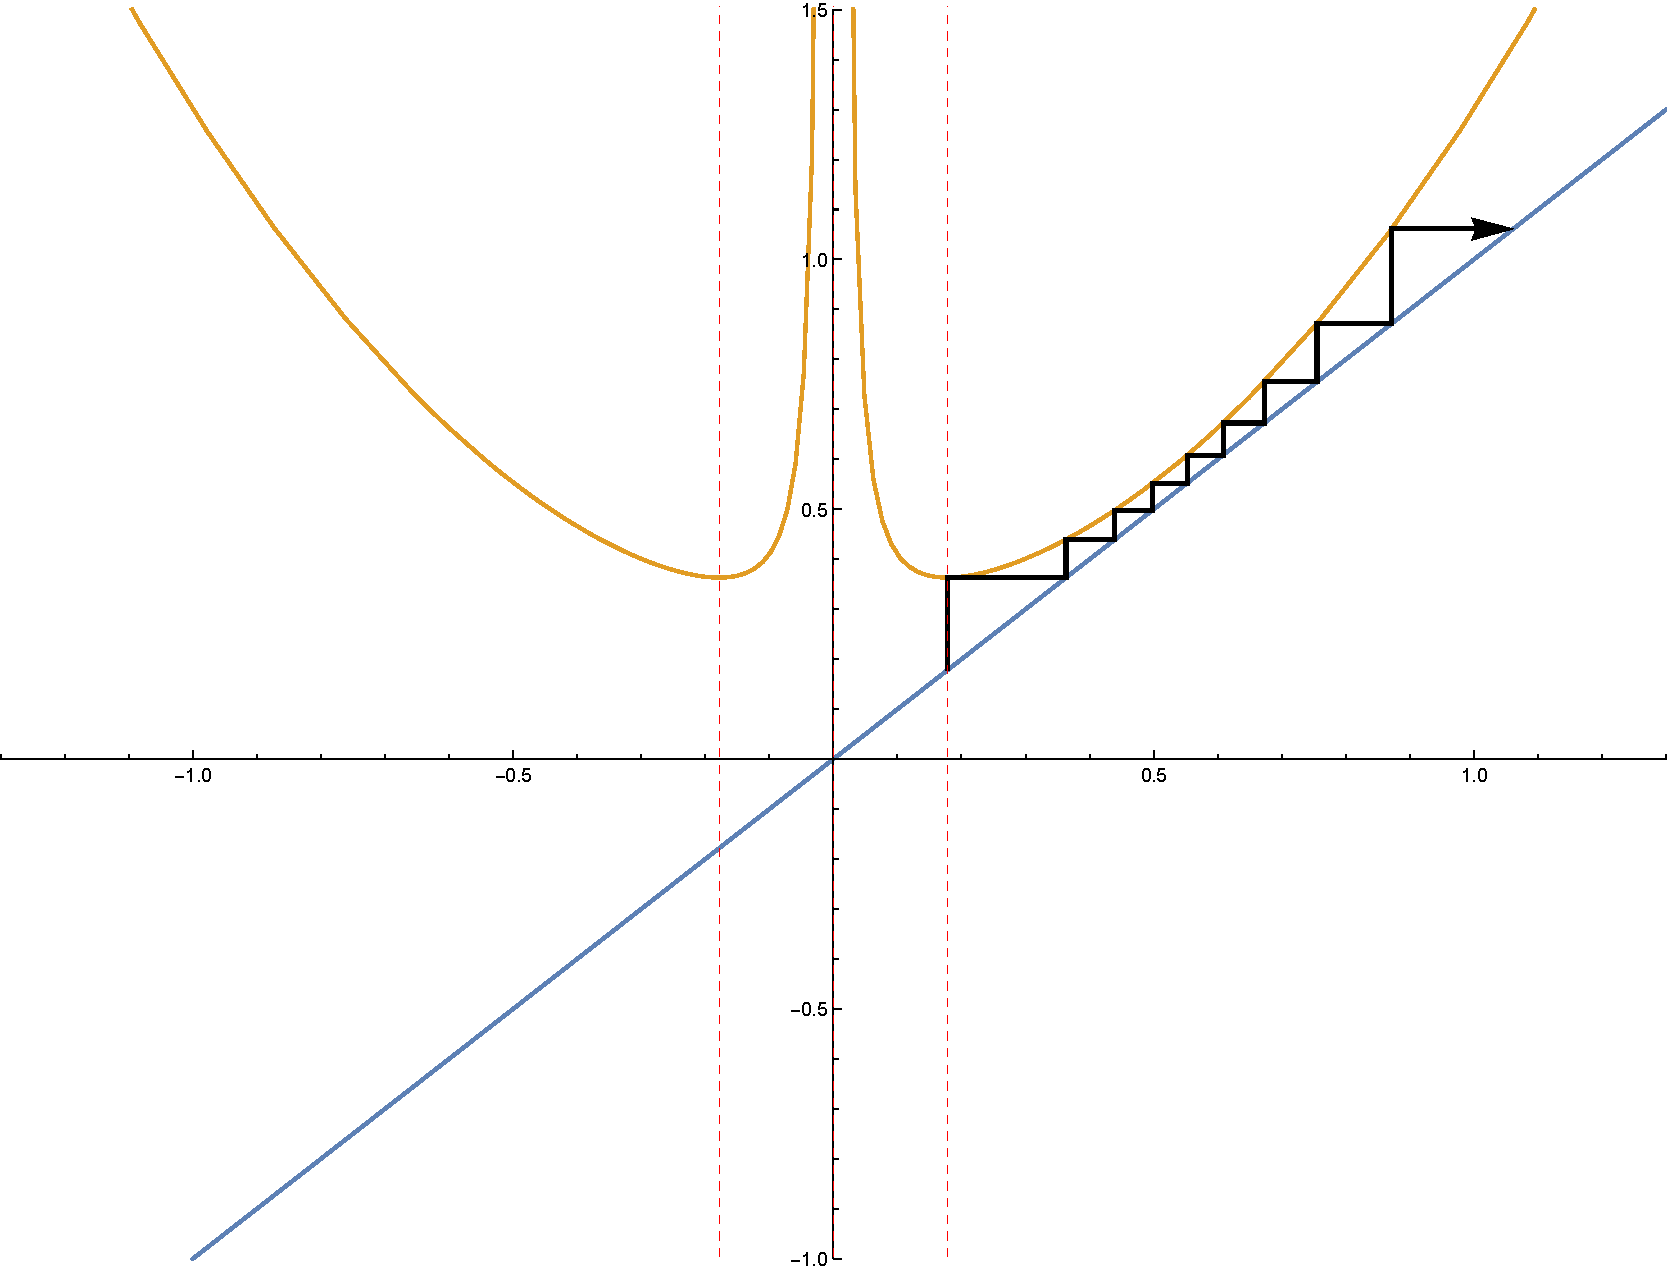
\includegraphics[width=\textwidth]{./img/plot03}
				\caption{$c \approx 0.3$}
		\end{subfigure}%
		\begin{subfigure}[b]{0.3\textwidth}
				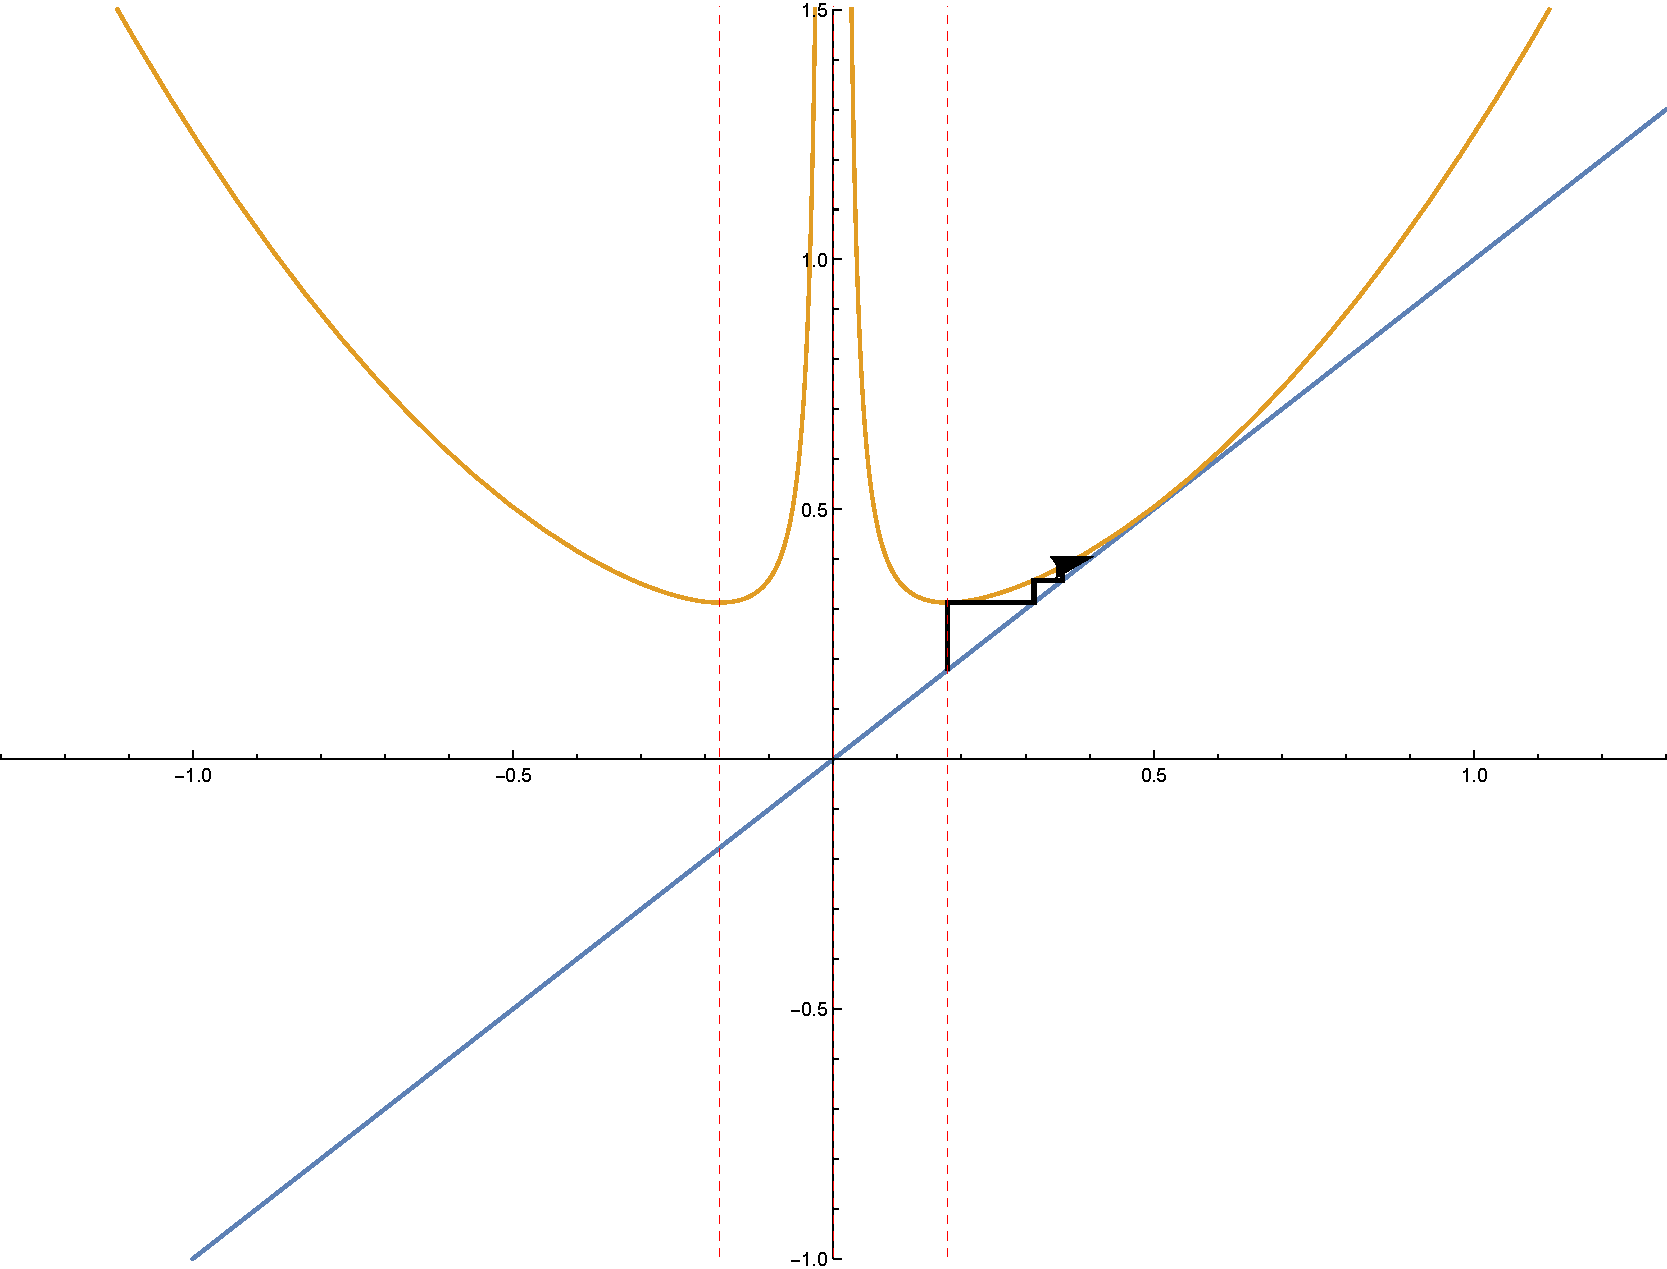
\includegraphics[width=\textwidth]{./img/plot025}
				\caption{$c \approx 0.24 \approx s_1^r$}
		\end{subfigure}
		\begin{subfigure}[b]{0.3\textwidth}
				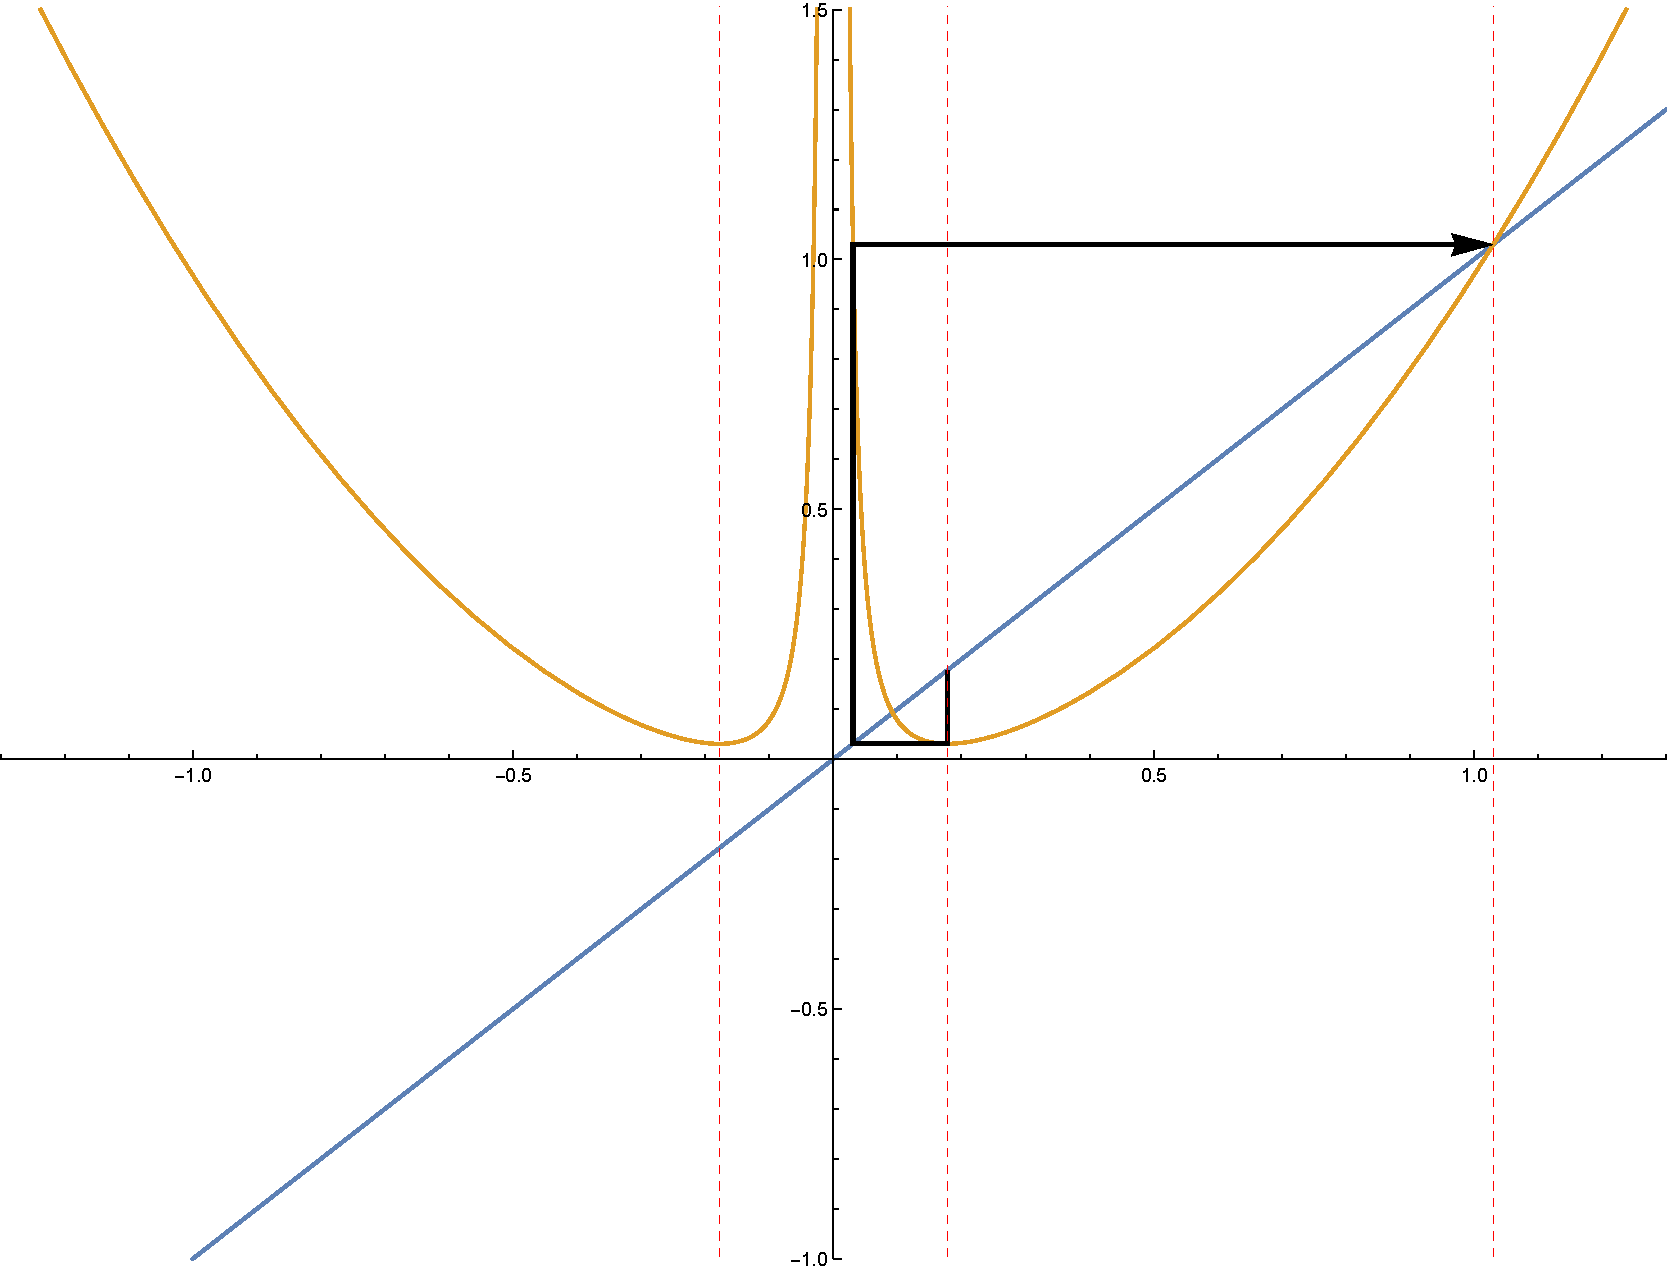
\includegraphics[width=\textwidth]{./img/plot-003255}
				\caption{$c \approx -.03255 \approx h_2^{CLP_c}$}
		\end{subfigure}

		\begin{subfigure}[b]{0.3\textwidth}
				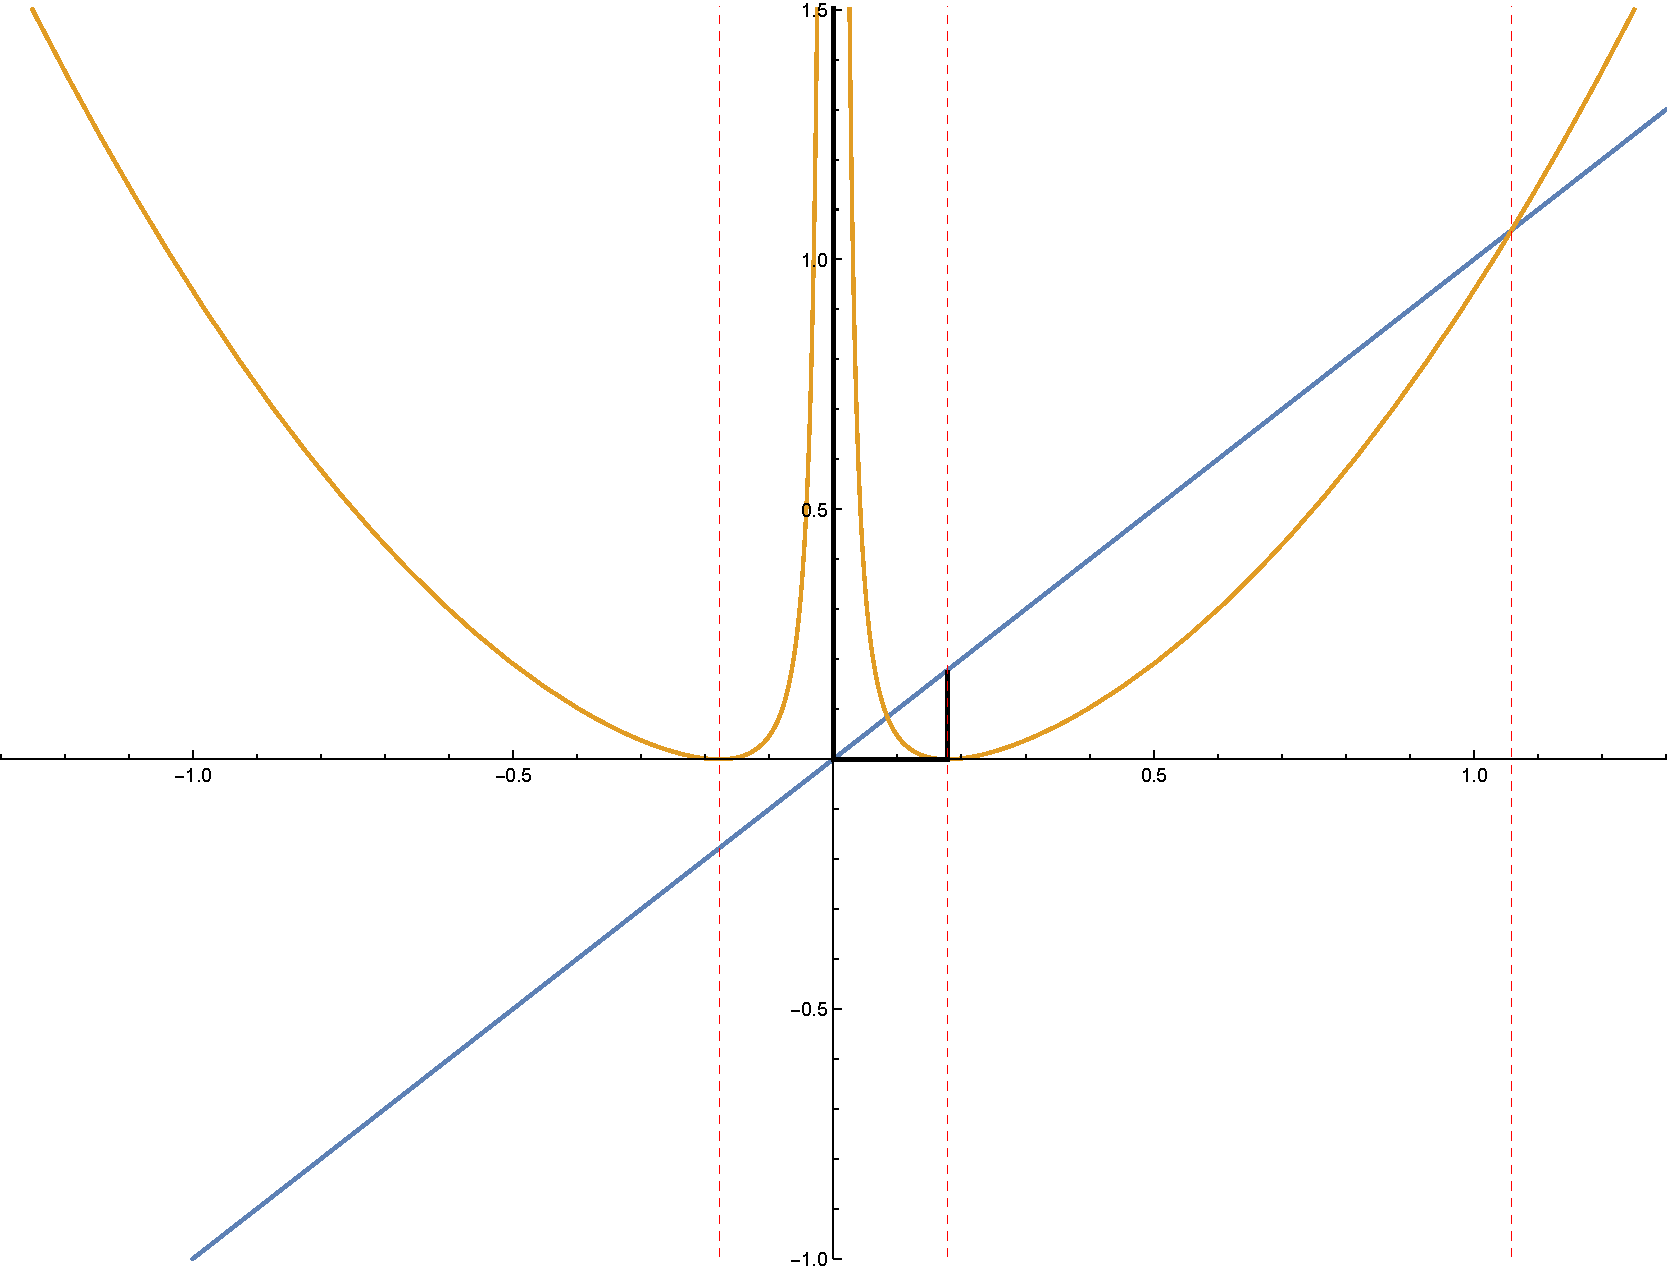
\includegraphics[width=\textwidth]{./img/plot-006355}
				\caption{$c \approx -.06335 \approx z_1^{C0}$}
		\end{subfigure}
		\begin{subfigure}[b]{0.3\textwidth}
				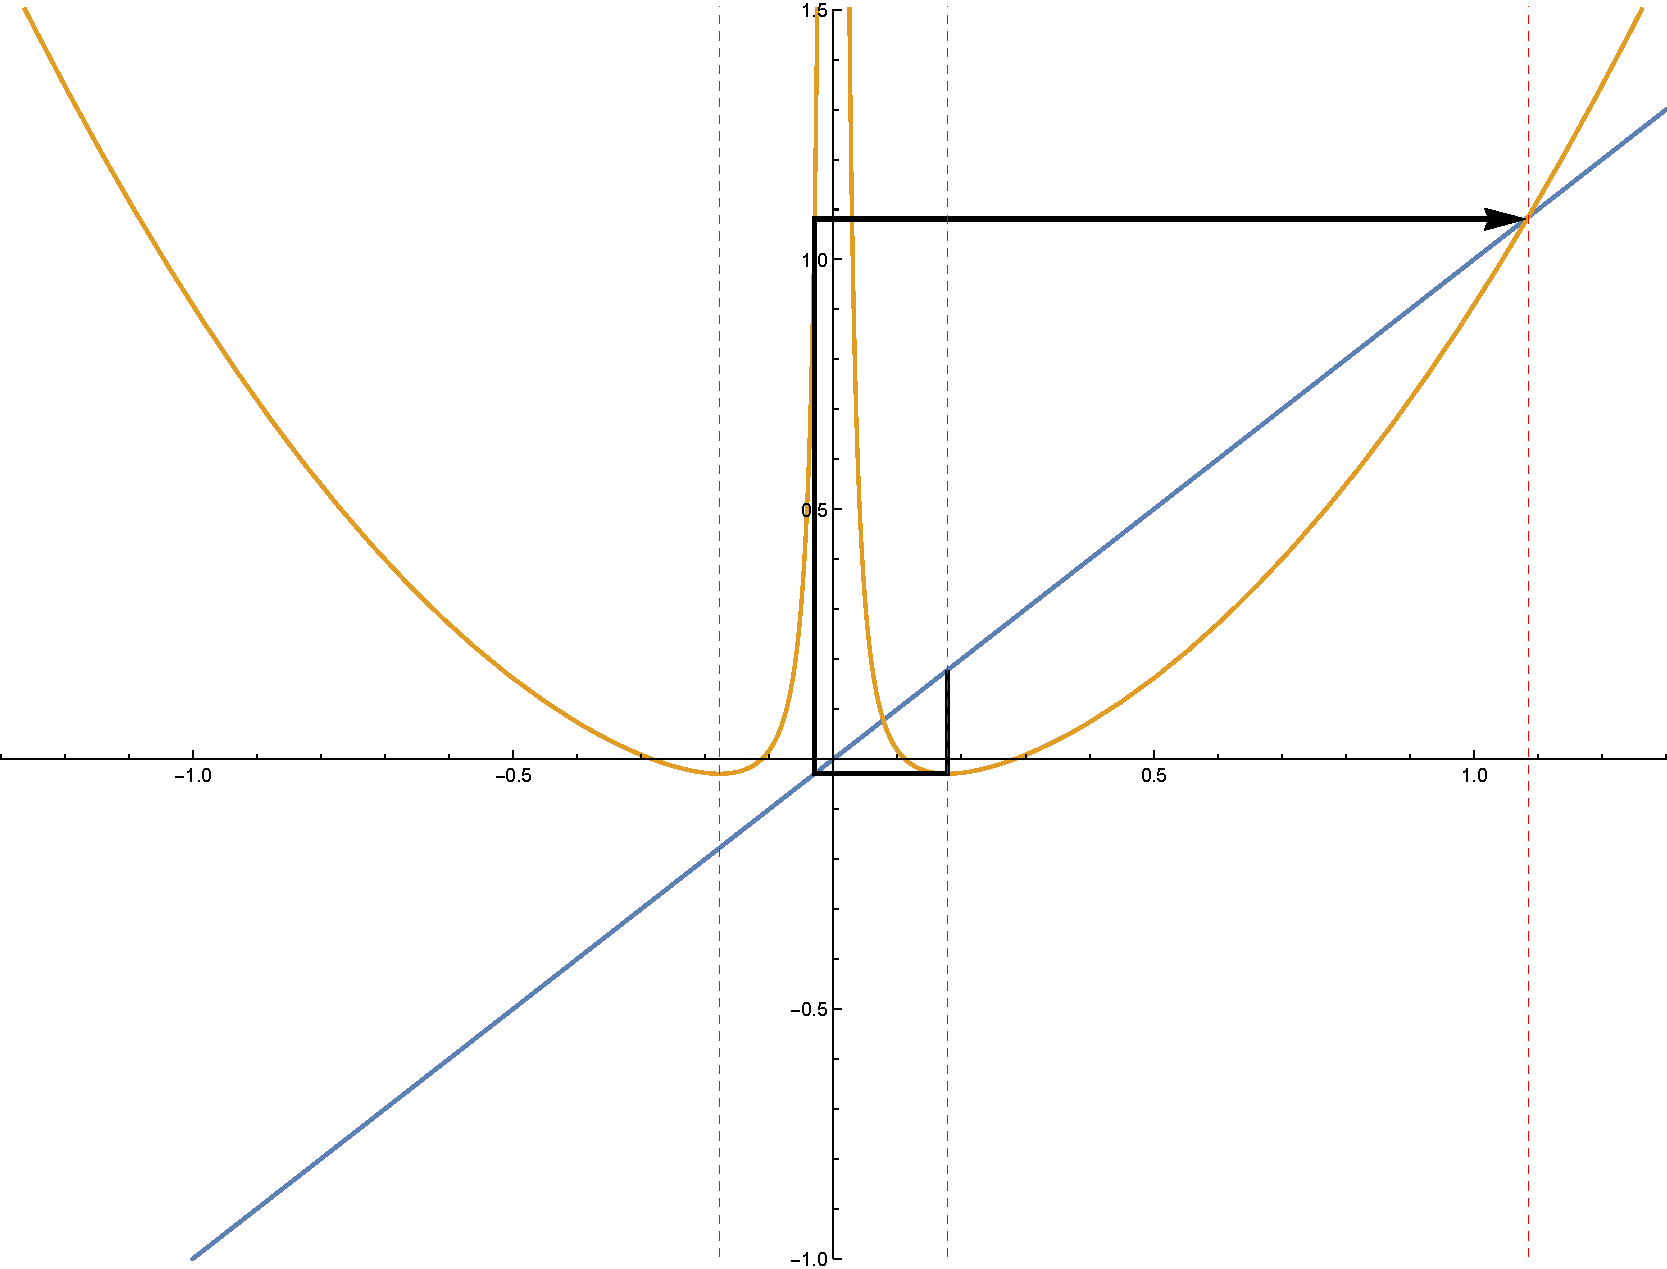
\includegraphics[width=\textwidth]{./img/plot-009245}
				\caption{$c \approx -.09245 \approx h_2^{CrP_c}$}
		\end{subfigure}
		\begin{subfigure}[b]{0.3\textwidth}
				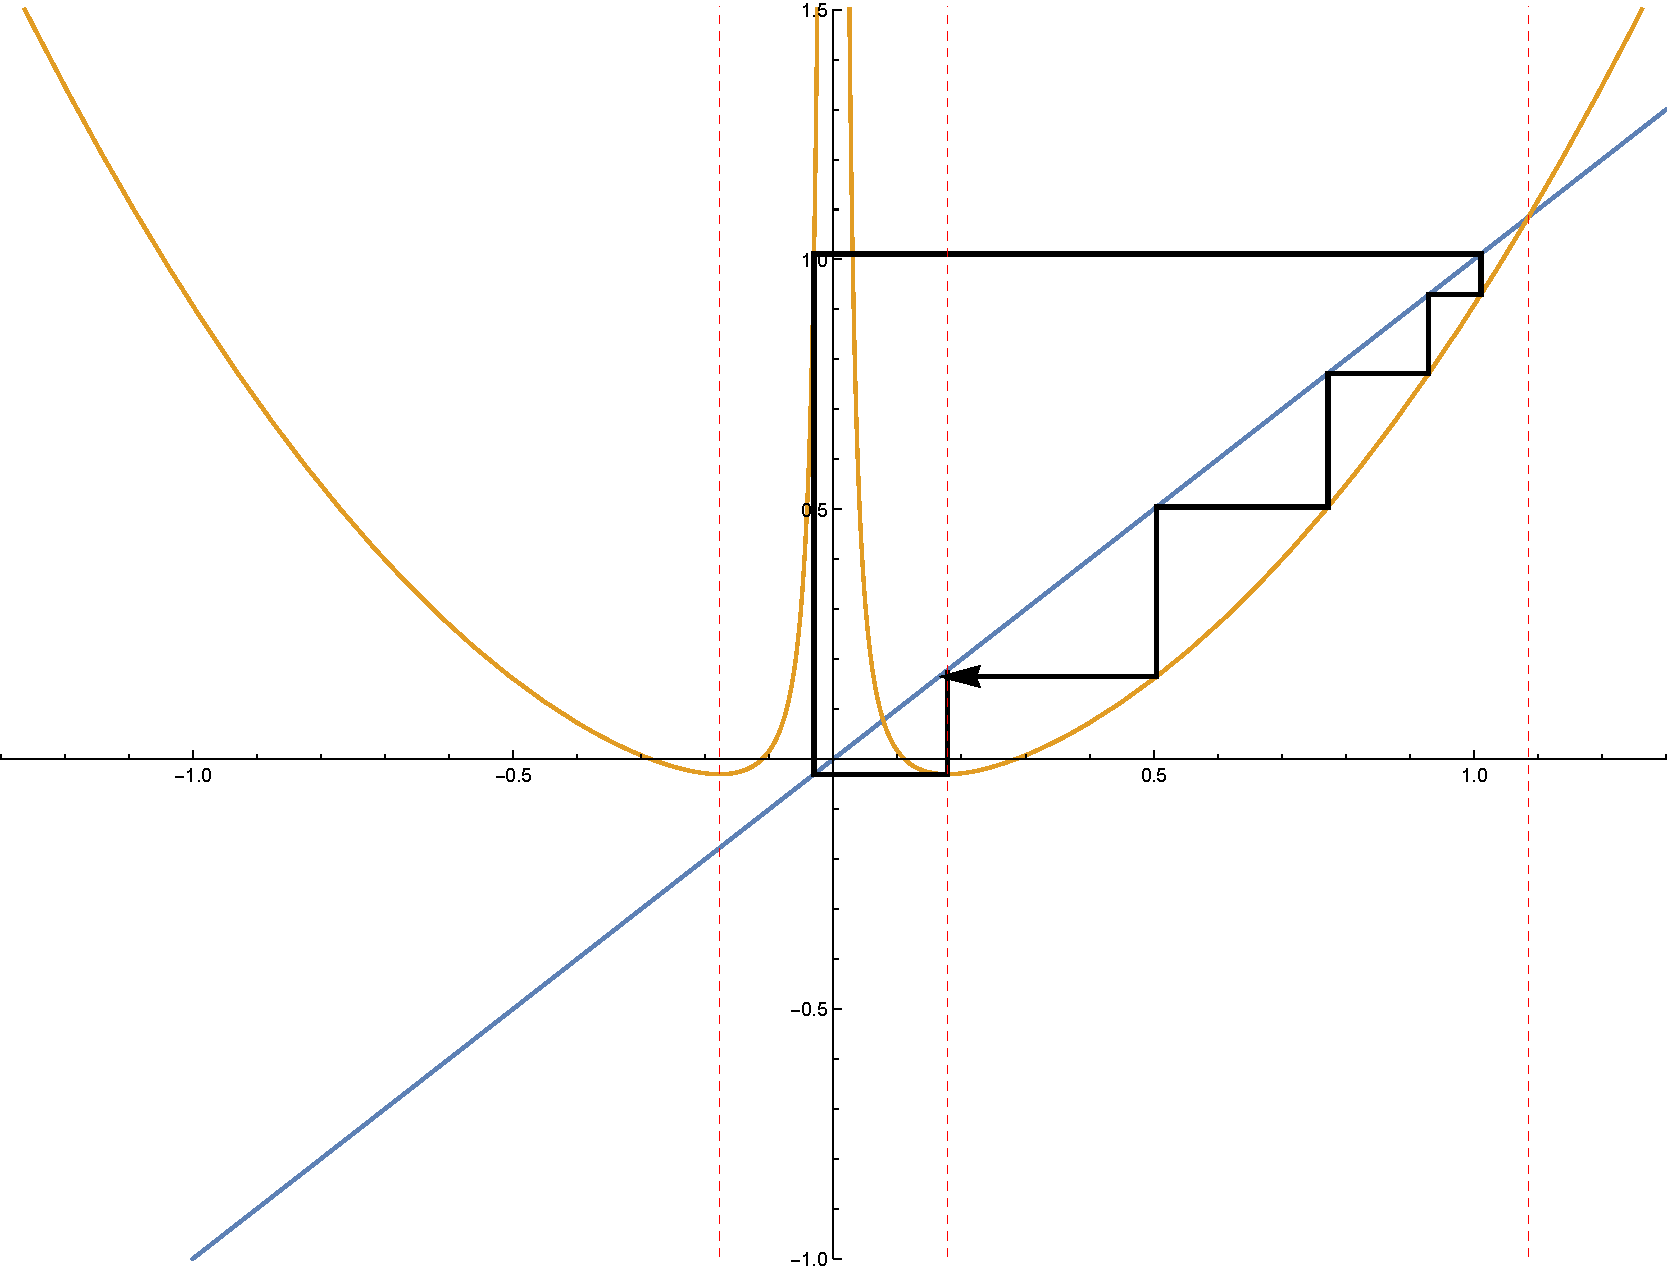
\includegraphics[width=\textwidth]{./img/plot-009335}
				\caption{$c \approx -.09335 \approx p_6^{CrFFFFC}$}
		\end{subfigure}

		\begin{subfigure}[b]{0.3\textwidth}
				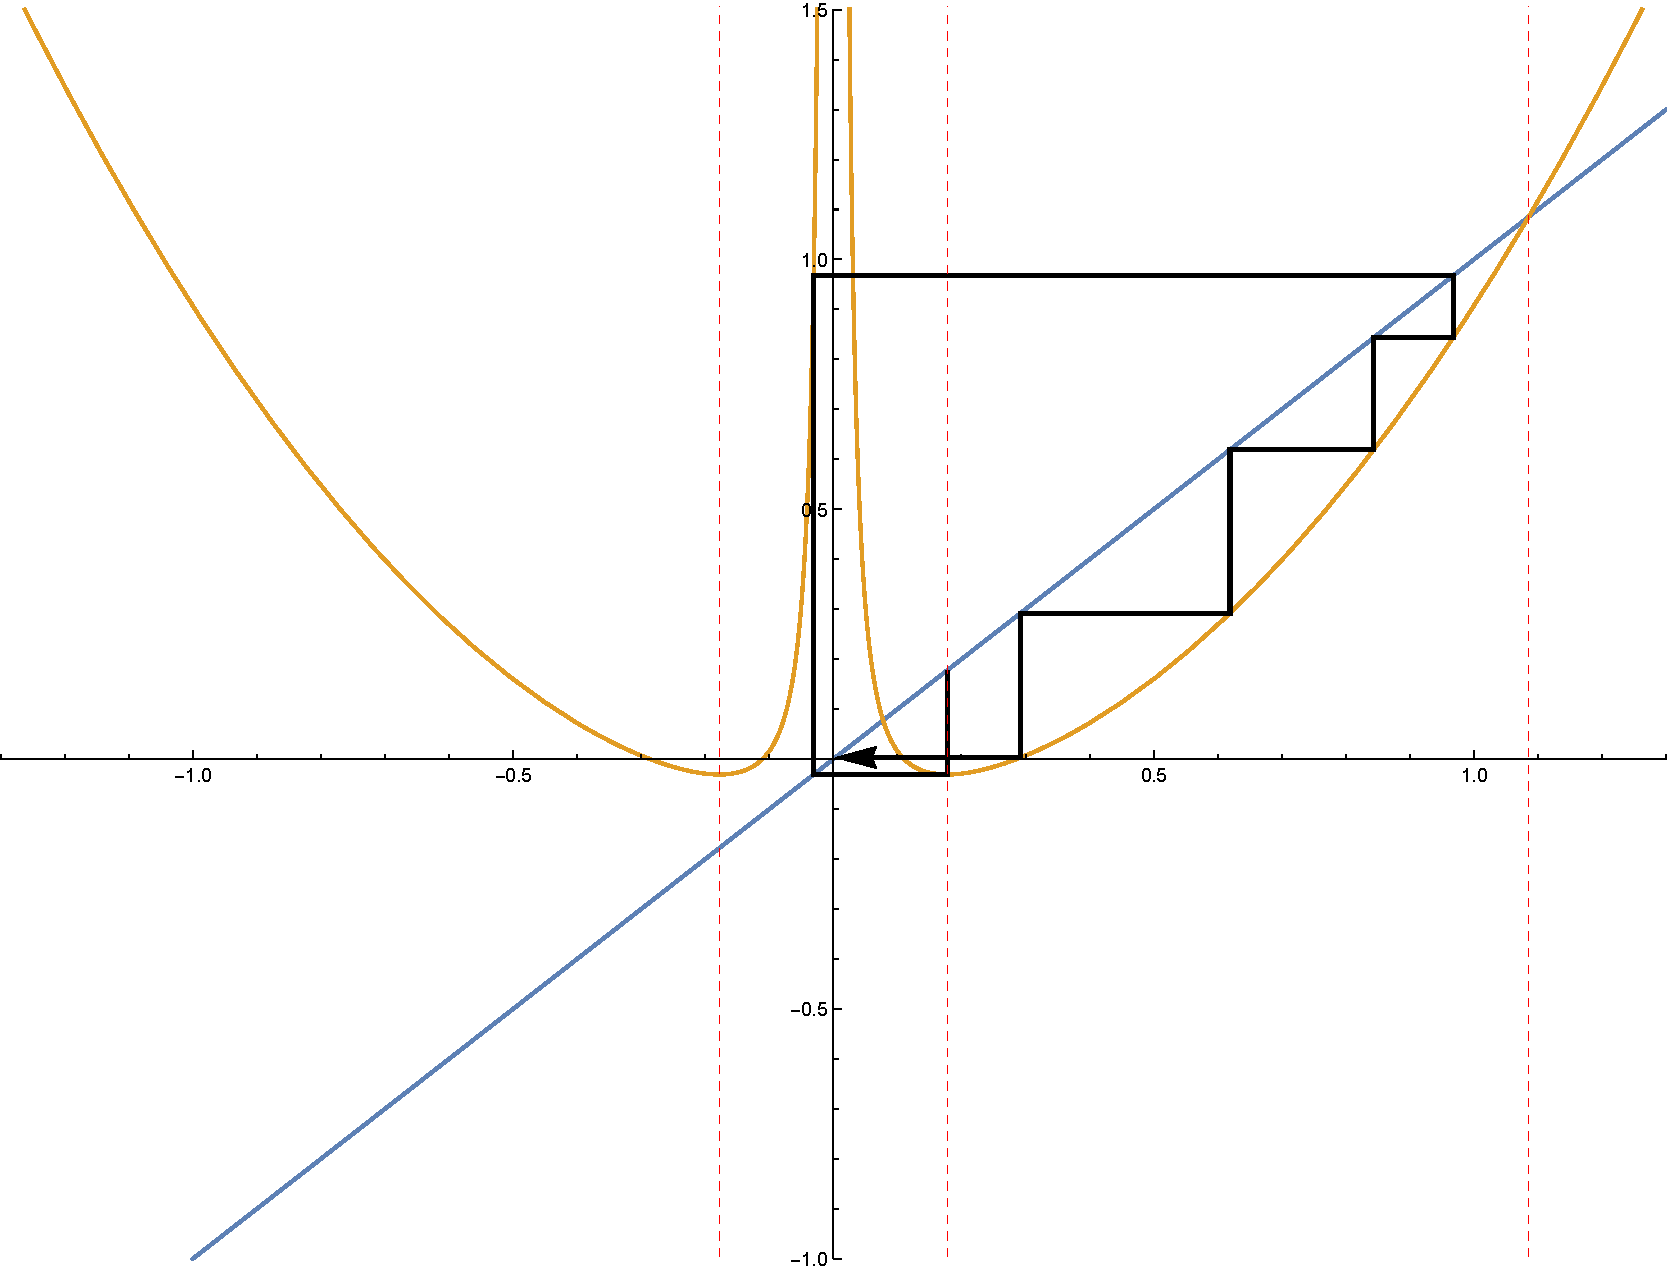
\includegraphics[width=\textwidth]{./img/plot-009395}
				\caption{$c \approx - .09395 \approx z_6^{CrFFFF0}$}
		\end{subfigure}
		\begin{subfigure}[b]{0.3\textwidth}
				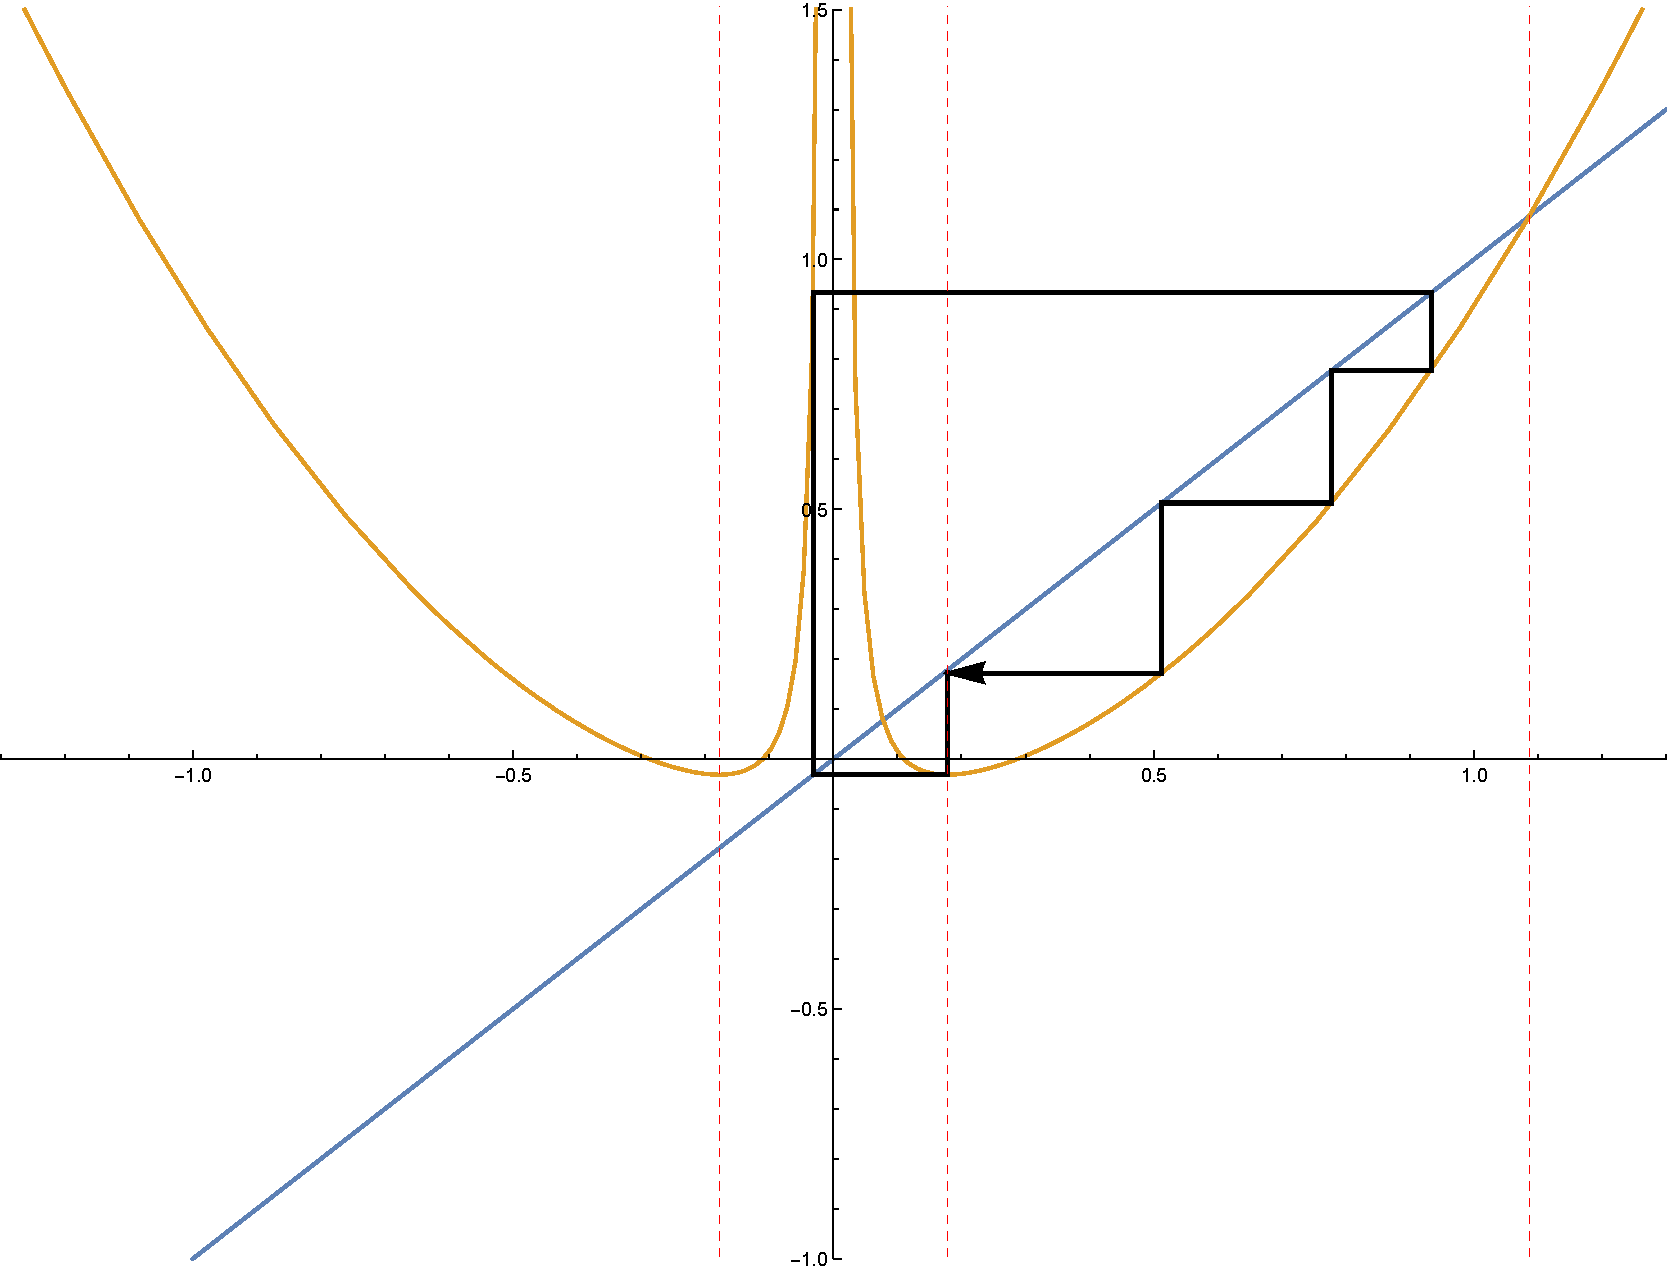
\includegraphics[width=\textwidth]{./img/plot-009445}
				\caption{$c \approx -.09445 \approx p_5^{CrFFFC}$}
		\end{subfigure}
		\begin{subfigure}[b]{0.3\textwidth}
				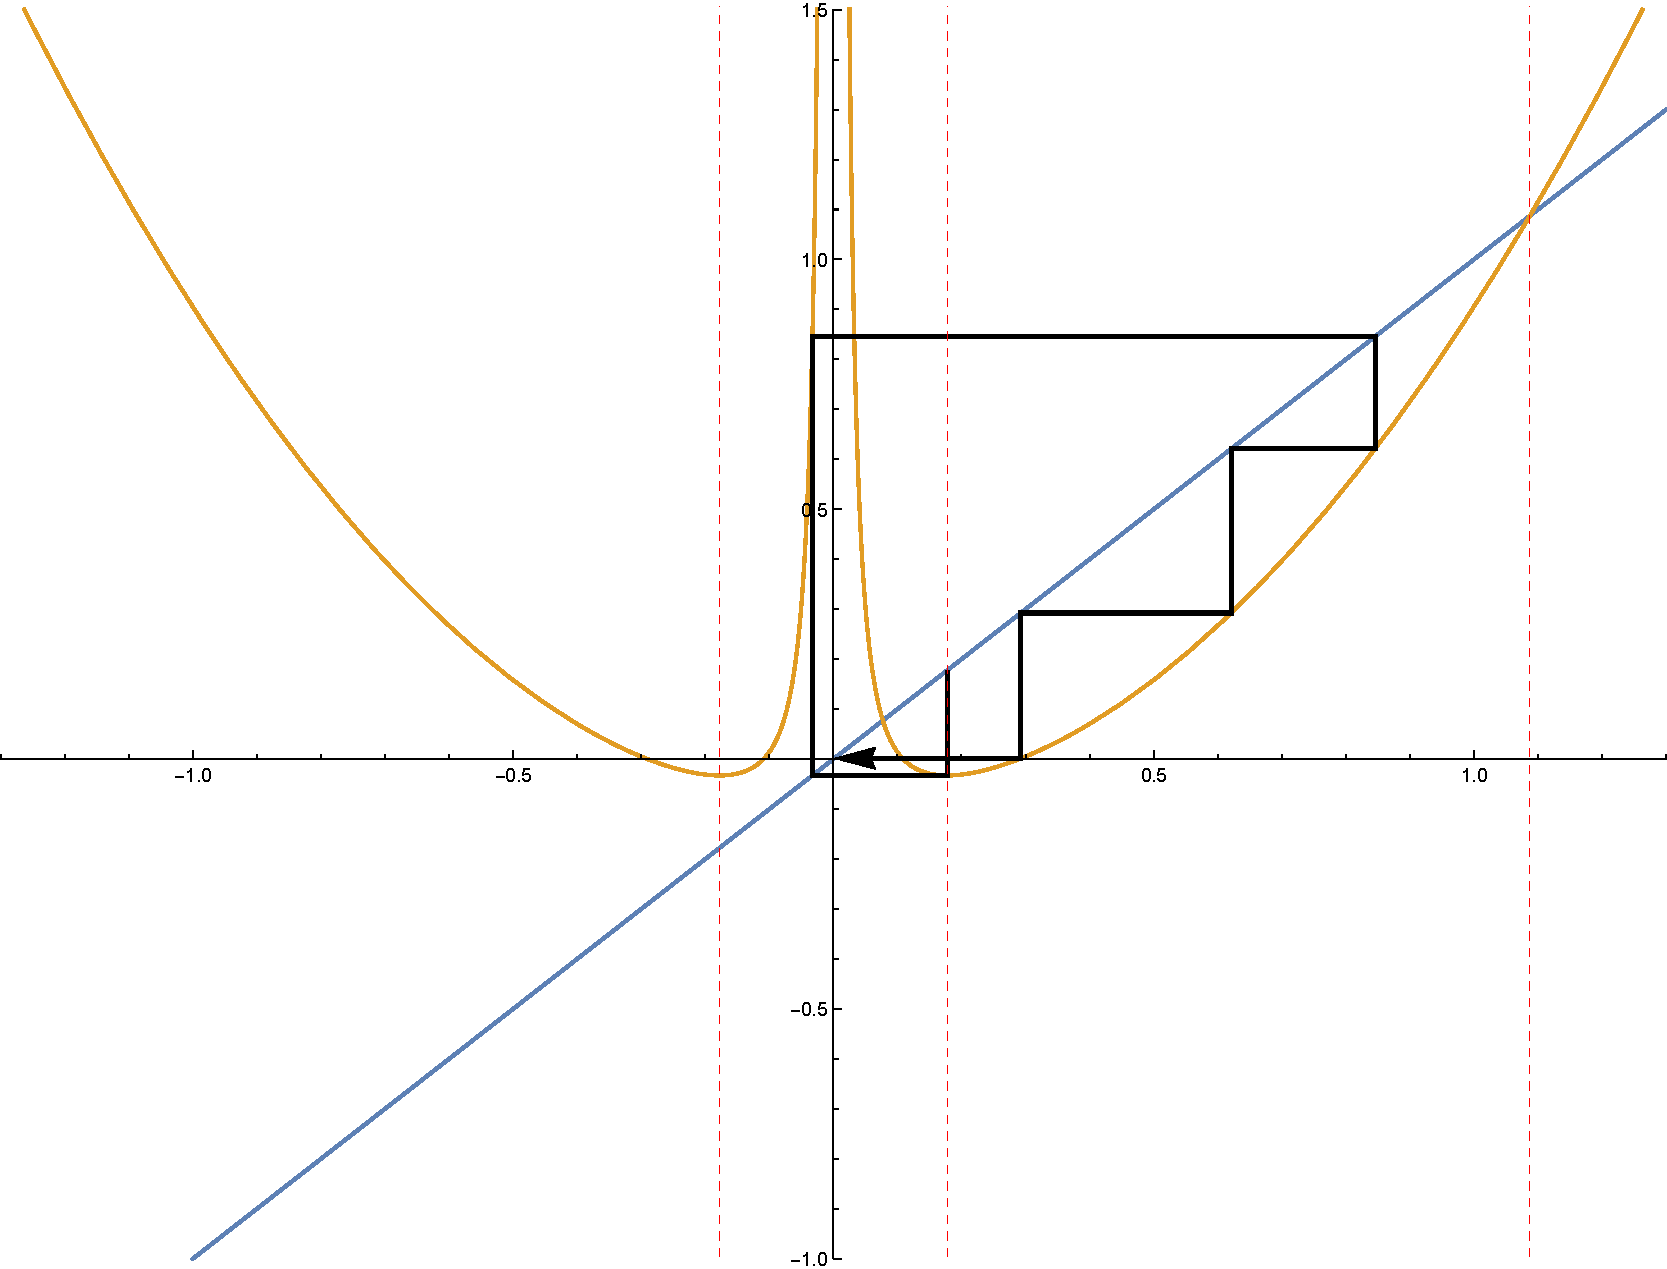
\includegraphics[width=\textwidth]{./img/plot-009585}
				\caption{$c \approx -.09585 \approx z_5^{CrFFF0}$}
		\end{subfigure}

		\begin{subfigure}[b]{0.3\textwidth}
				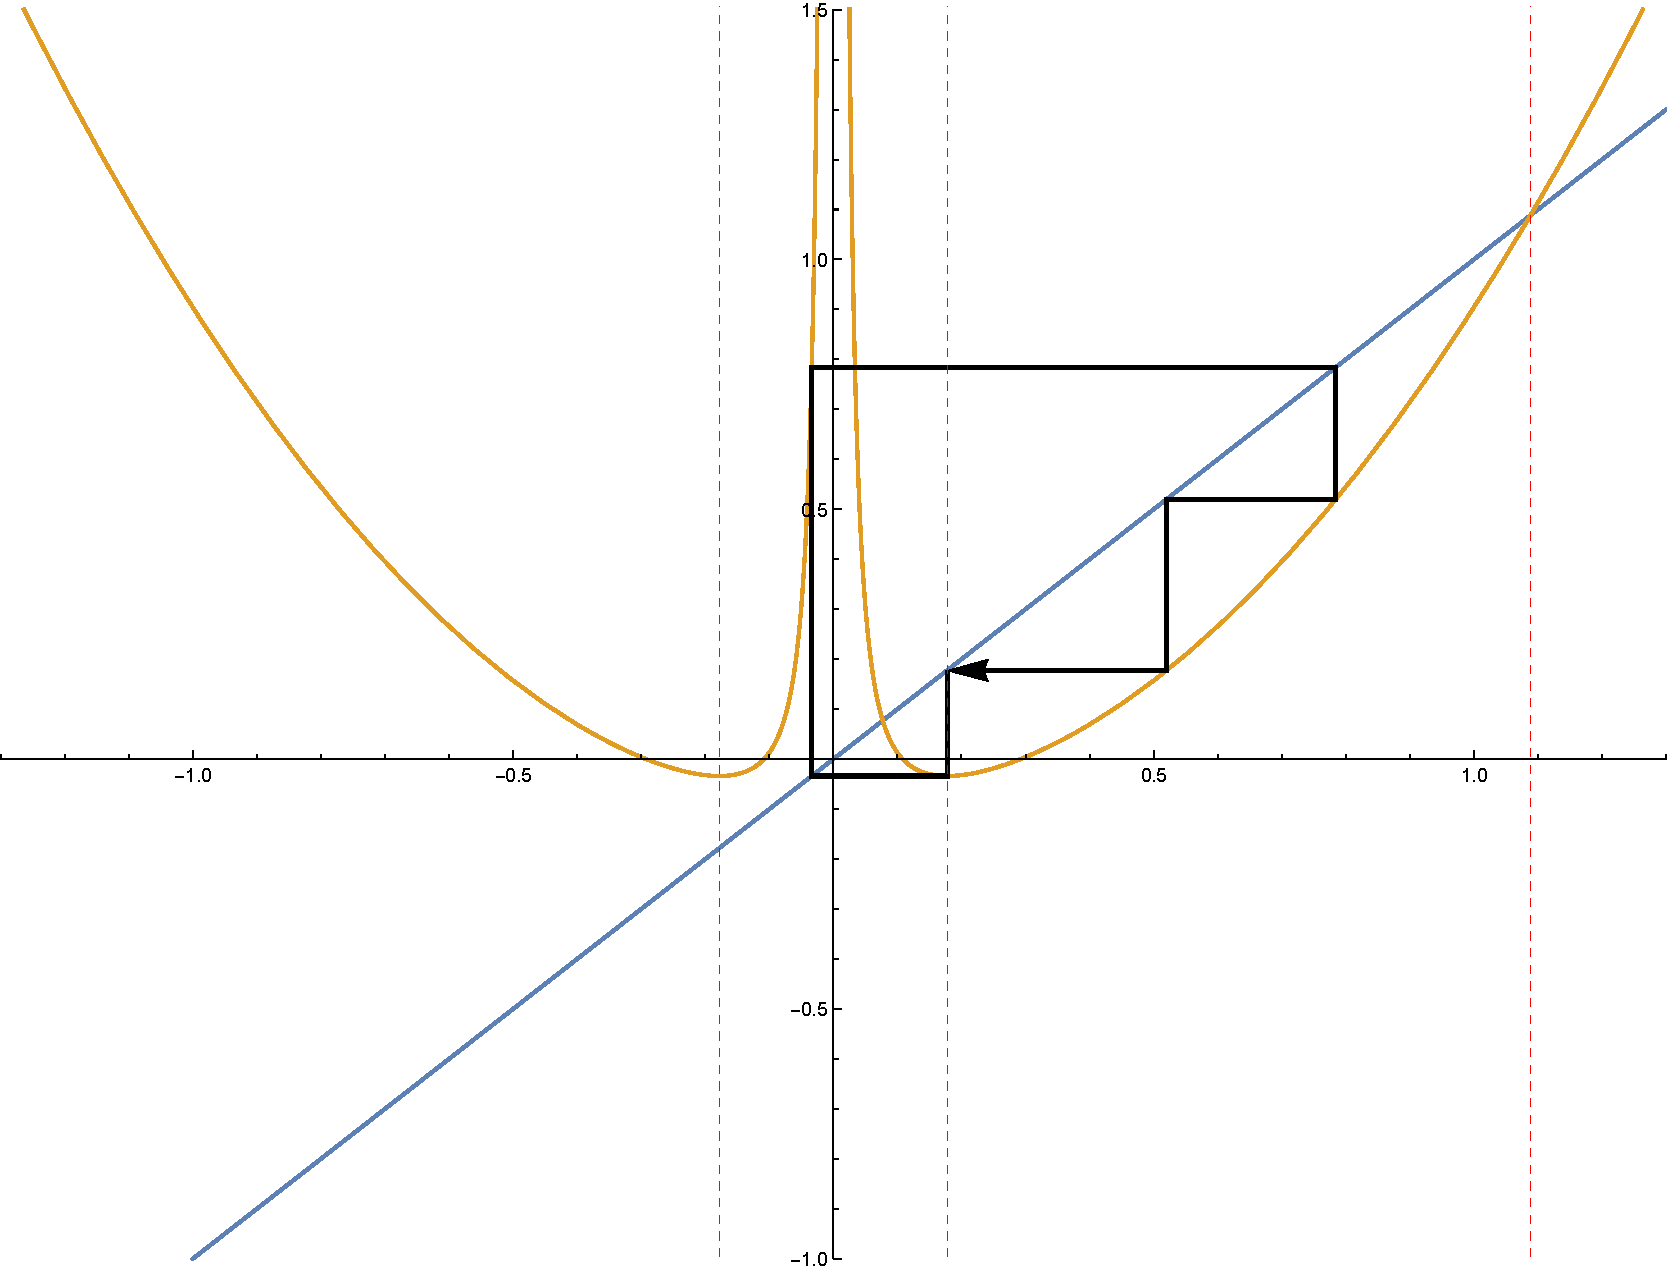
\includegraphics[width=\textwidth]{./img/plot-009695}
				\caption{$c \approx -.09695 \approx p_4^{CrFFC}$}
		\end{subfigure}
		\begin{subfigure}[b]{0.3\textwidth}
				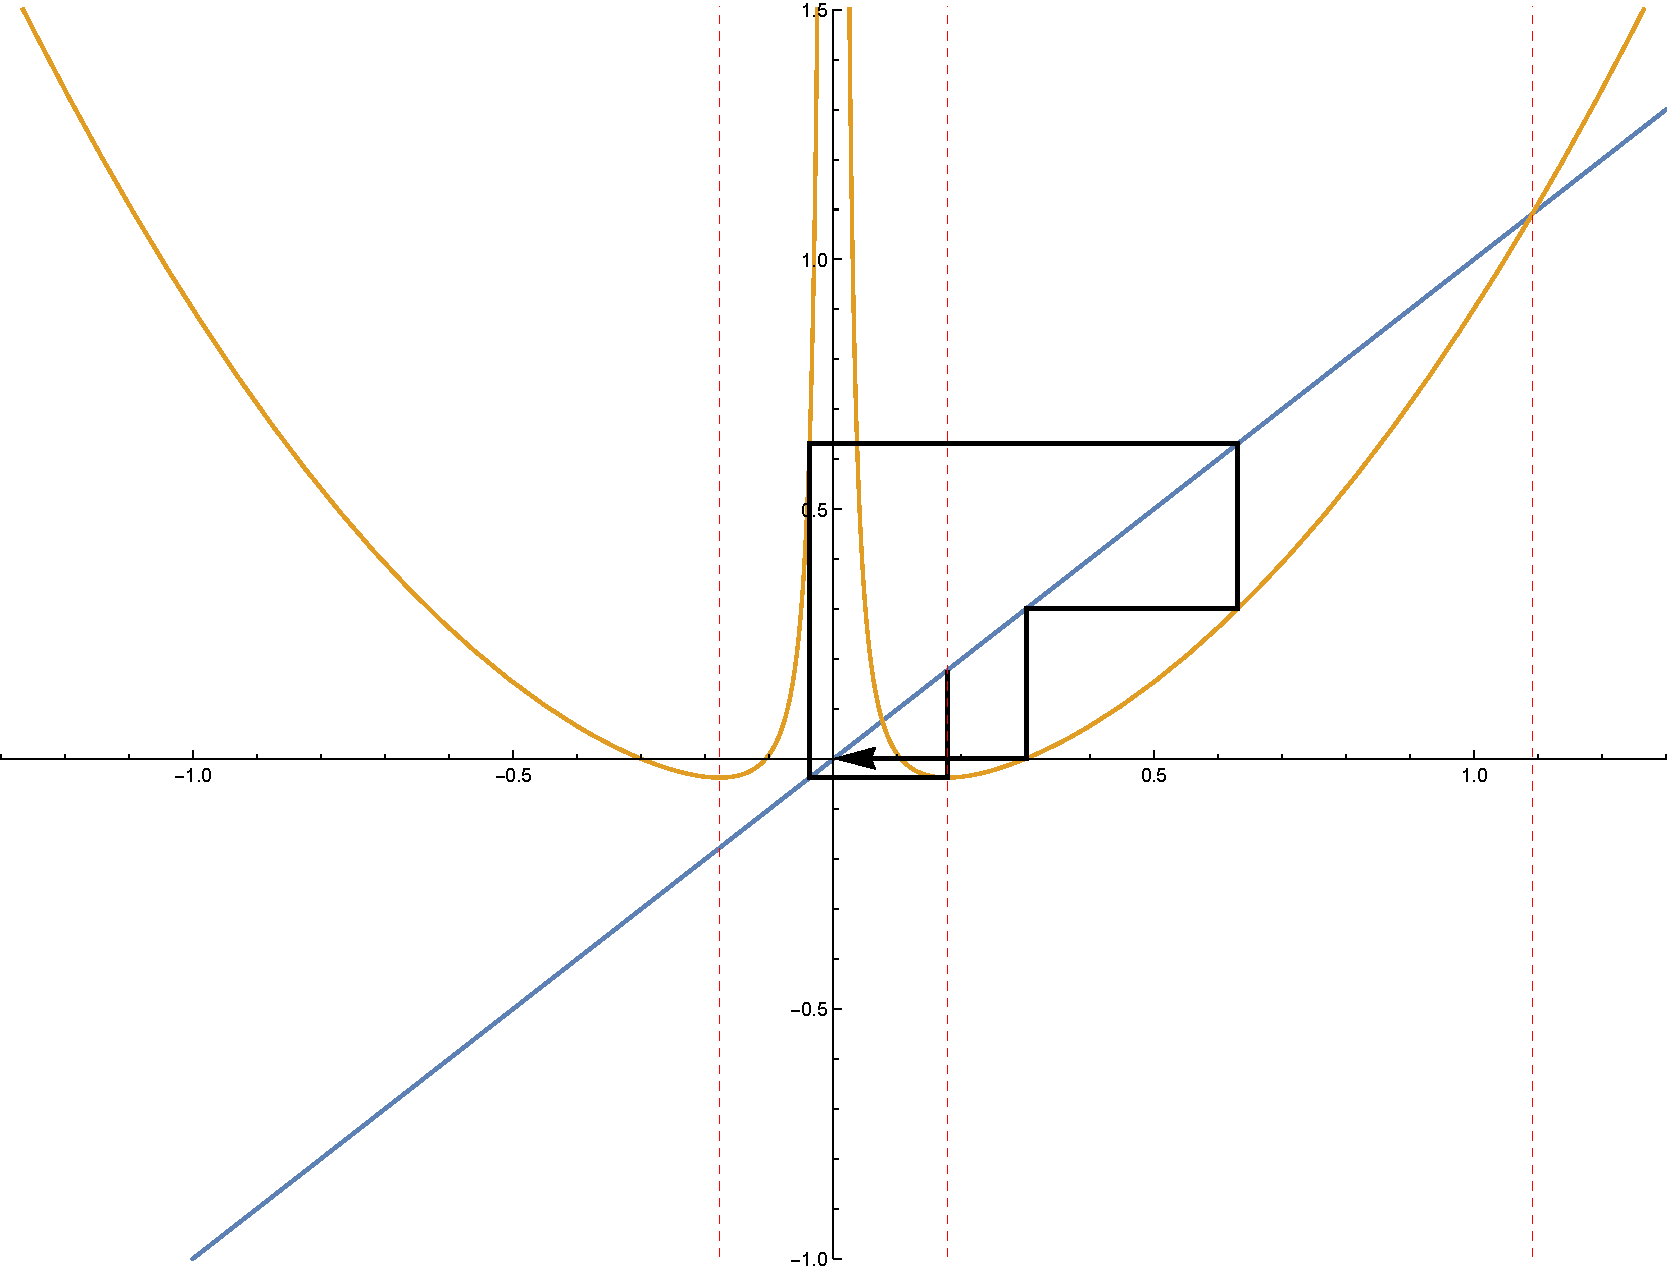
\includegraphics[width=\textwidth]{./img/plot-010025}
				\caption{$c \approx -.10025 \approx z_4^{CrFF0}$}
		\end{subfigure}
		\begin{subfigure}[b]{0.3\textwidth}
				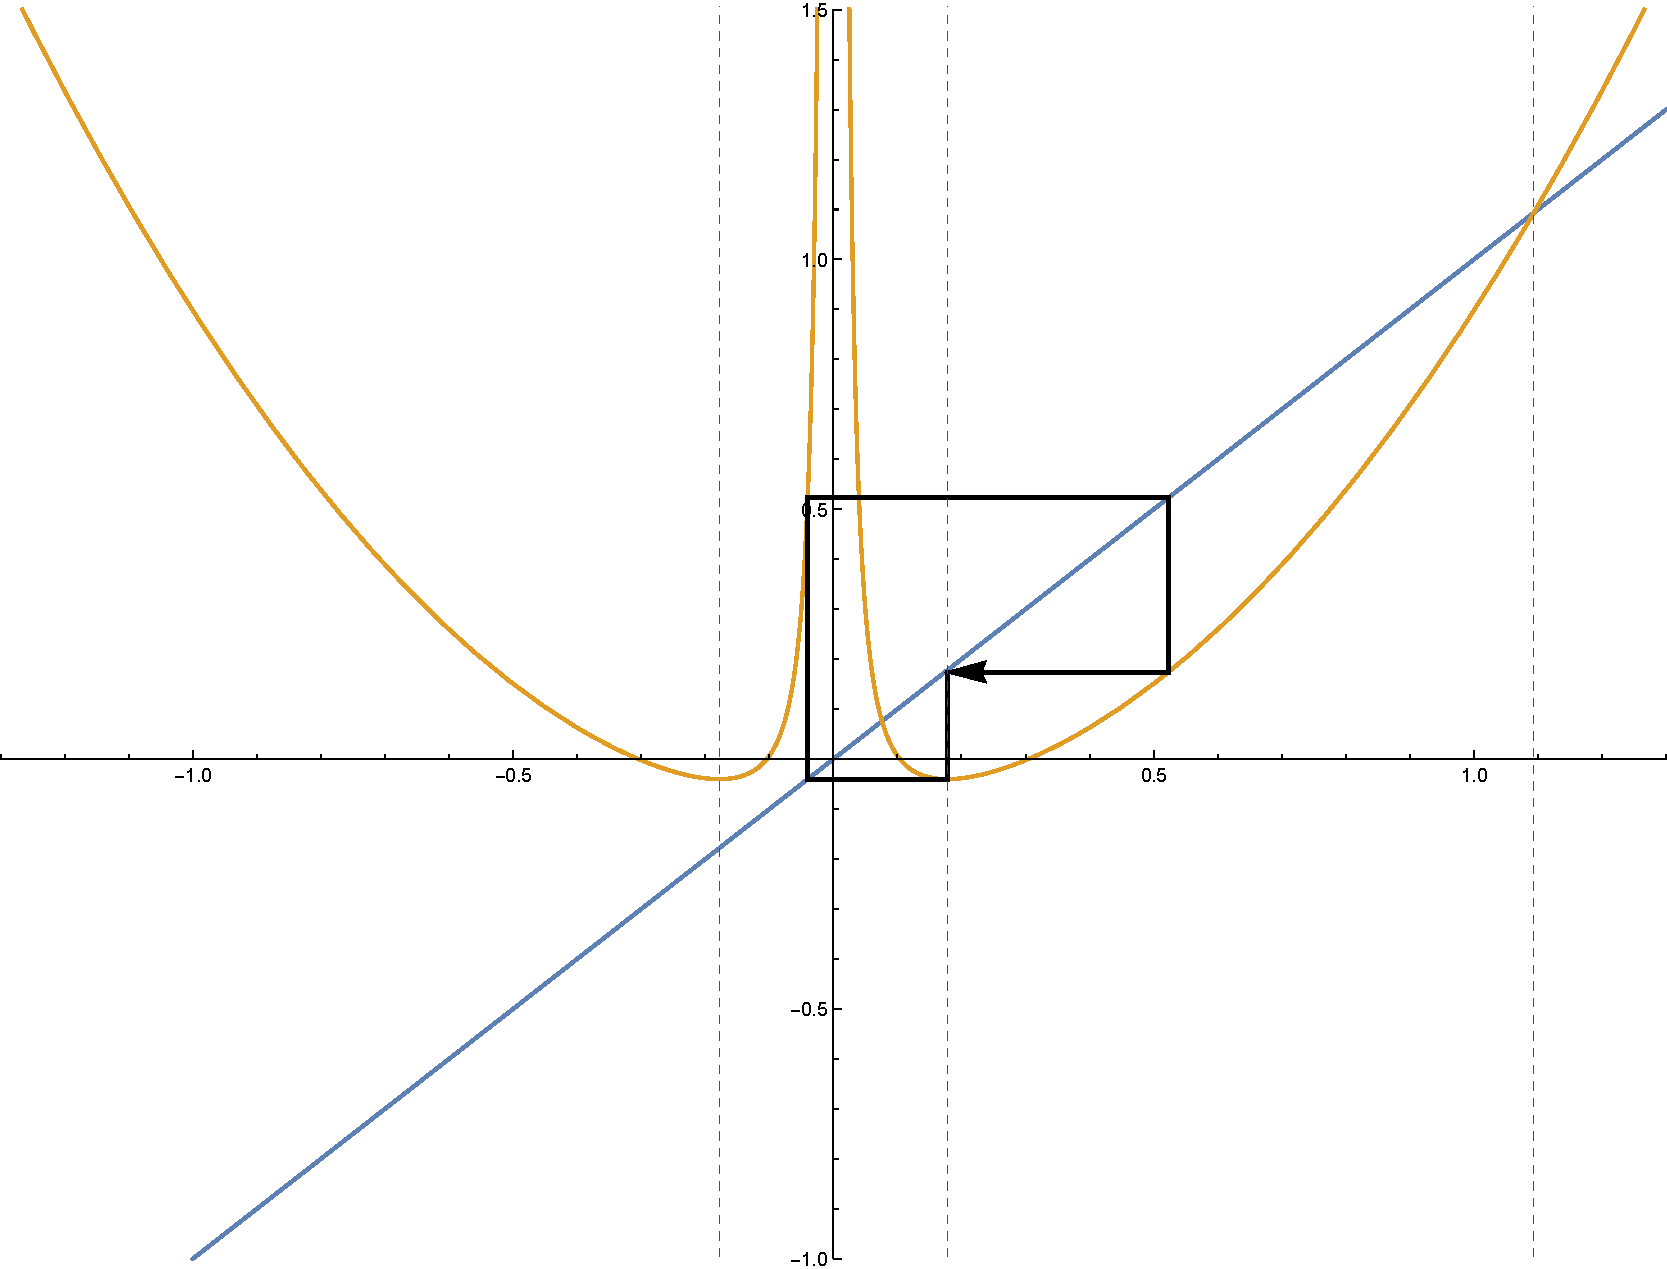
\includegraphics[width=\textwidth]{./img/plot-010325}
				\caption{$c \approx - .10325 \approx p_3^{CrFC}$}
		\end{subfigure}

		\begin{subfigure}[b]{0.3\textwidth}
				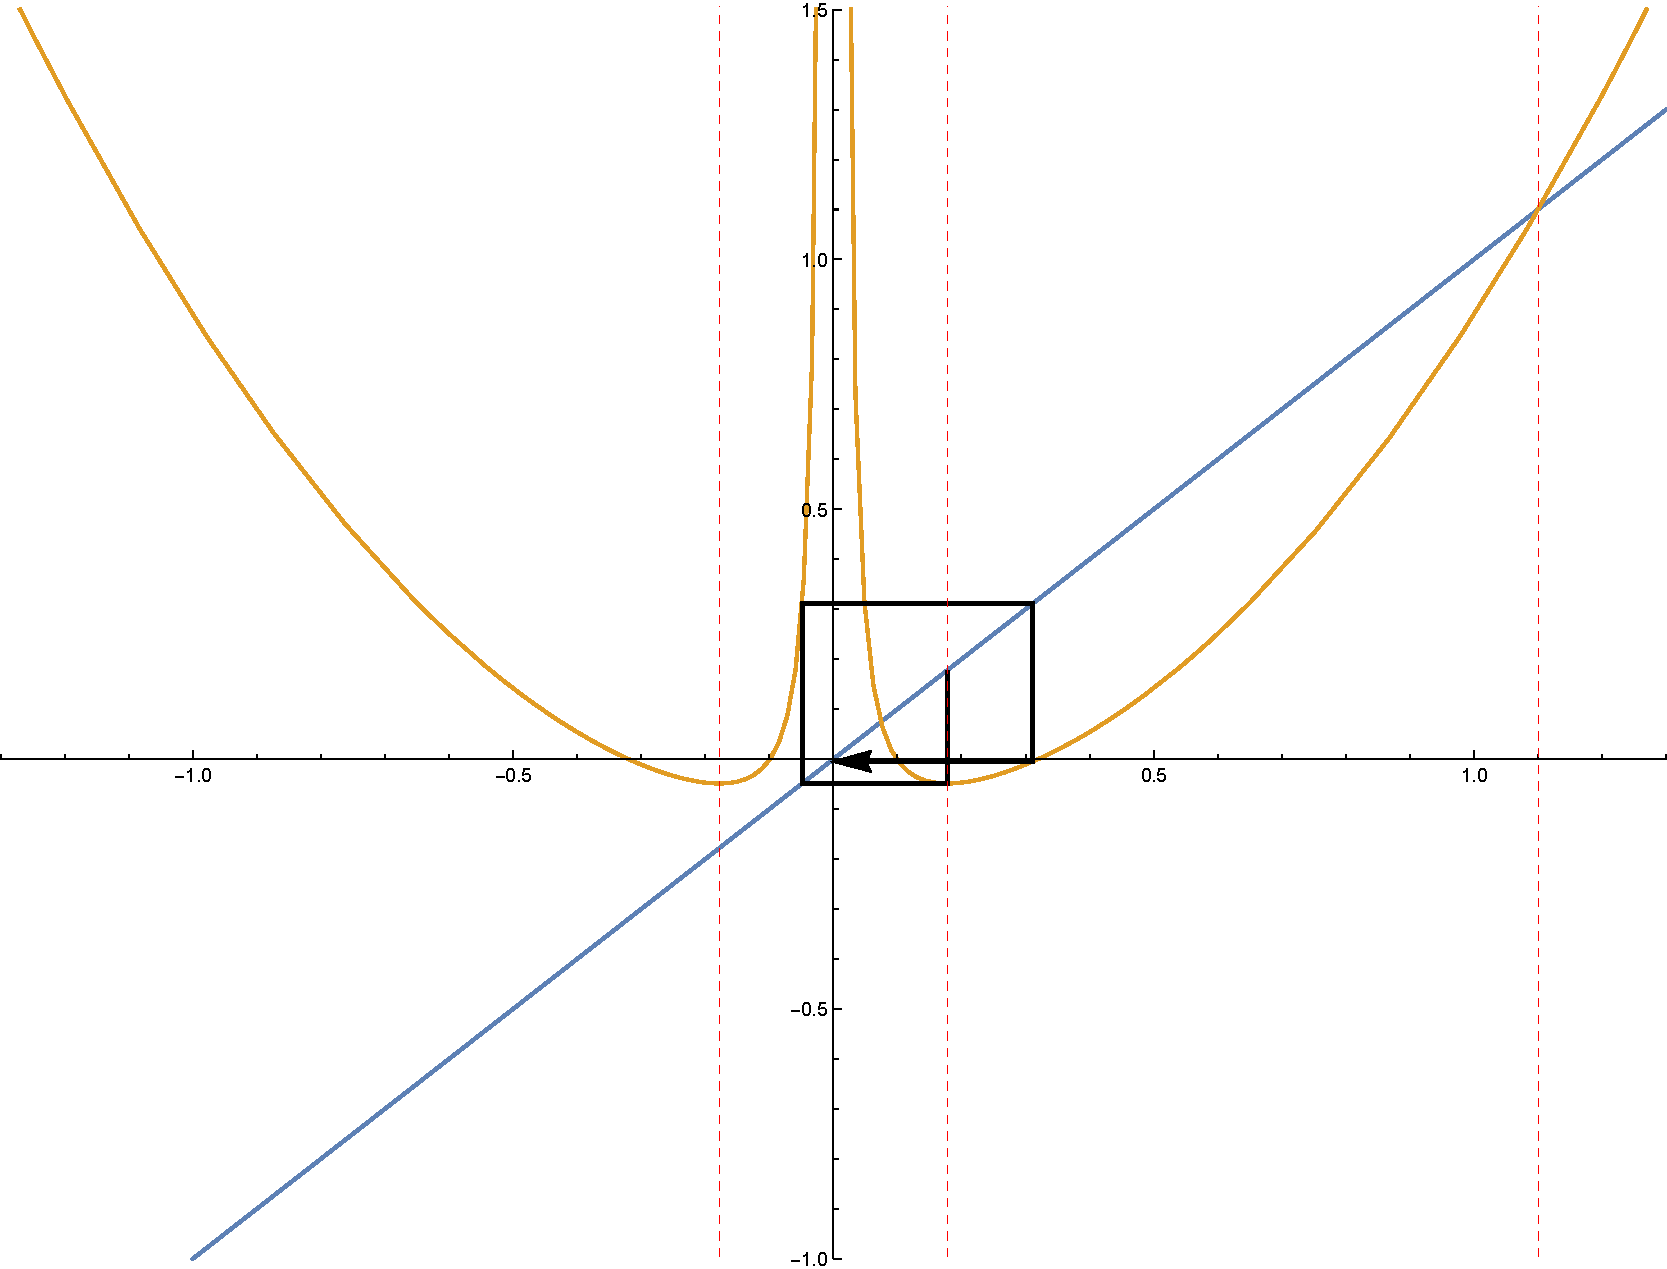
\includegraphics[width=\textwidth]{./img/plot-0112}
				\caption{$c \approx -.112 \approx z_3^{CrF0}$}
		\end{subfigure}
		\begin{subfigure}[b]{0.3\textwidth}
				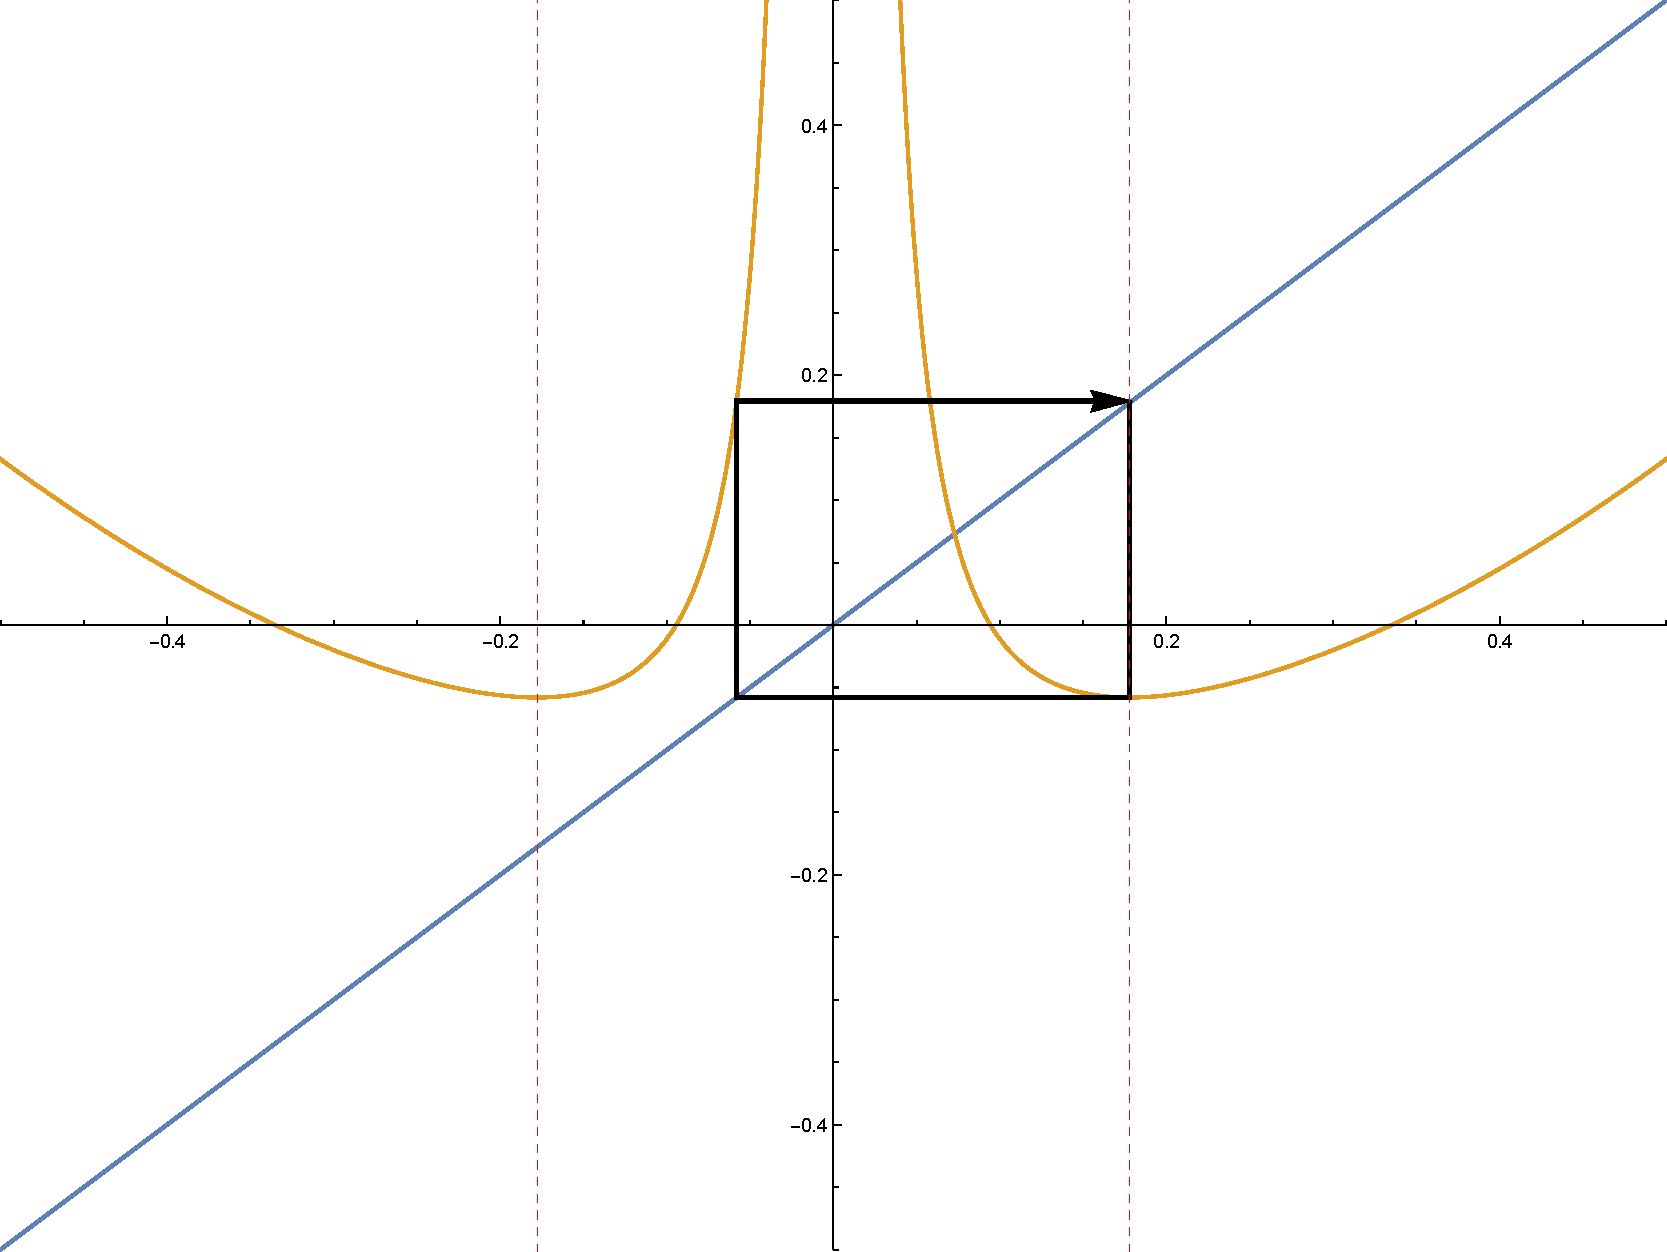
\includegraphics[width=\textwidth]{./img/plot-012125}
				\caption{$c \approx - .12125 \approx p_2^{CrC}$}
		\end{subfigure}
		\begin{subfigure}[b]{0.3\textwidth}
				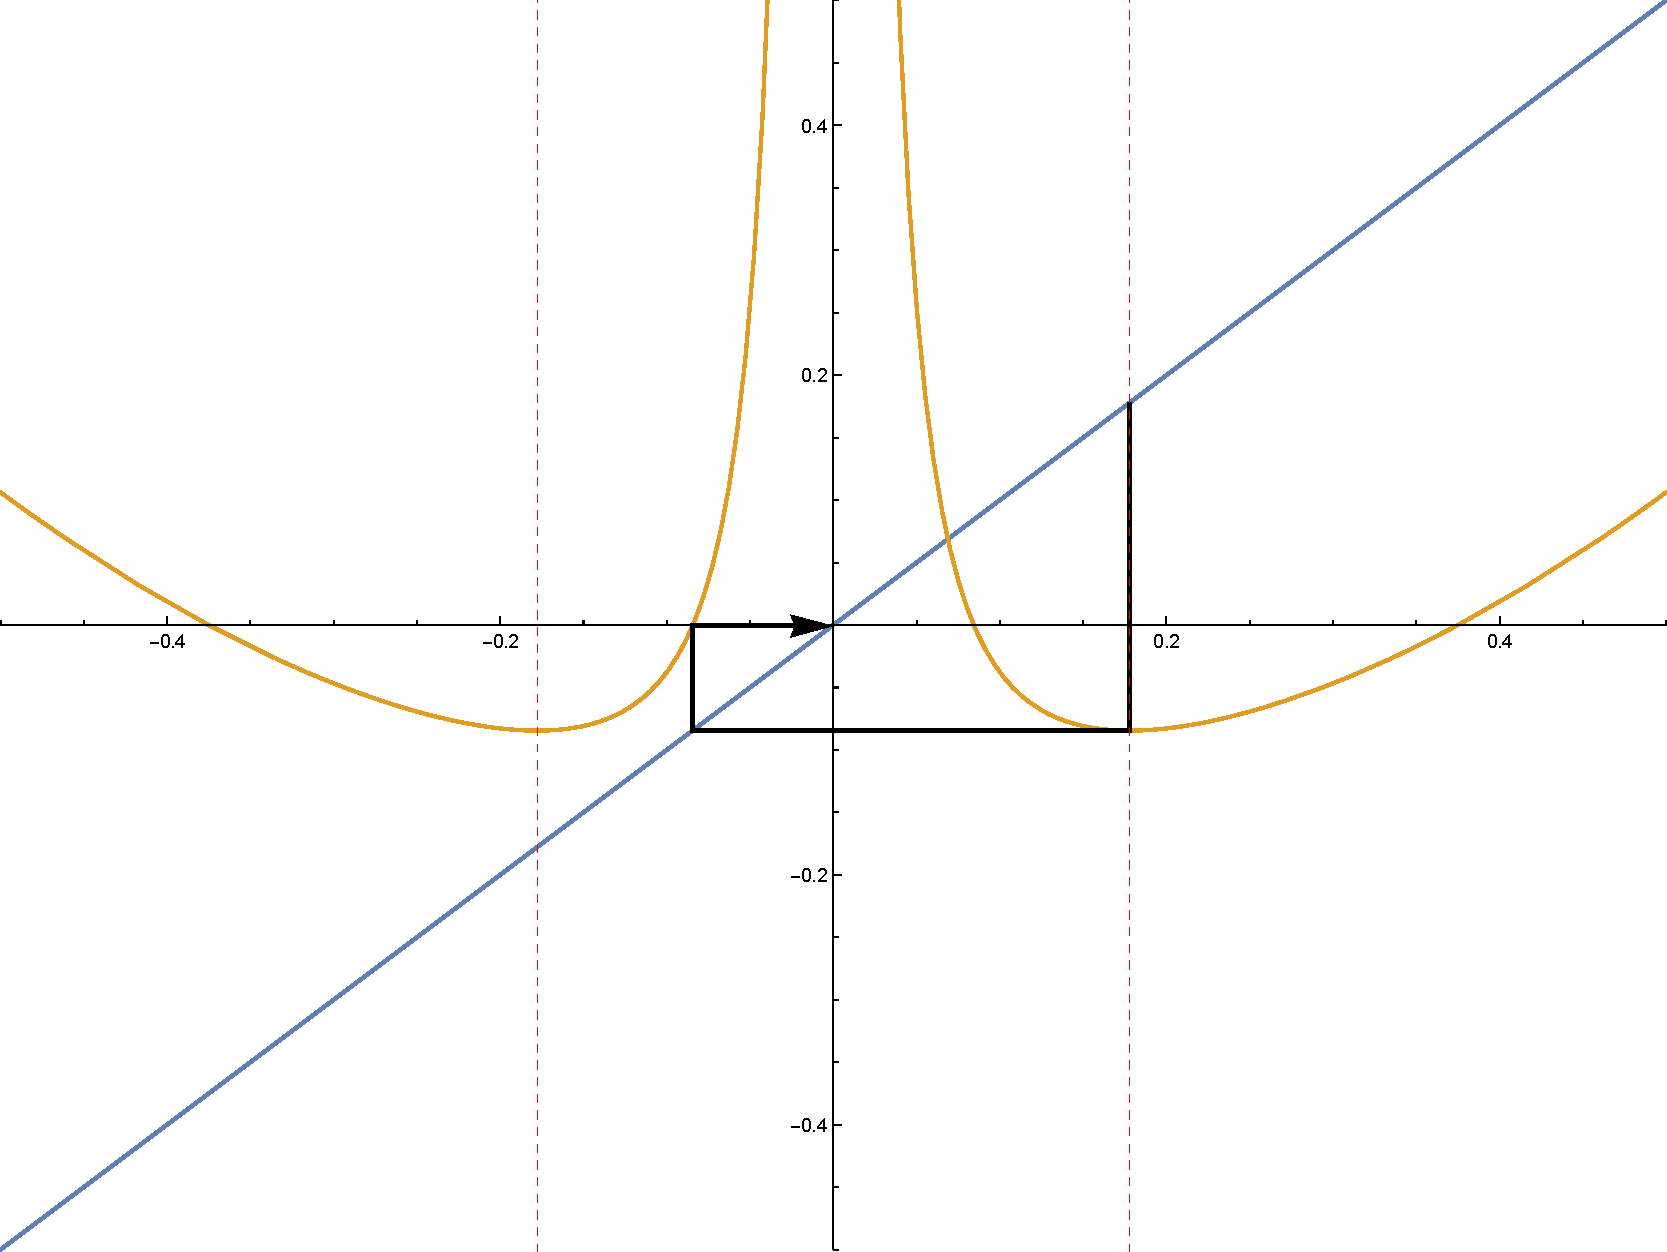
\includegraphics[width=\textwidth]{./img/plot-014778}
				\caption{$c \approx -.14778 \approx z_2^{Cr0}$}
		\end{subfigure}
		% \begin{subfigure}[b]{0.3\textwidth}
		% 		\includegraphics[width=\textwidth]{./img/plot-}
		% 		\caption{Seventh iterate of $f_c (C)$ added along with the parameter value of its prezero orbit}
		% 		\label{fig:cplot6S}
		% \end{subfigure}
		% \begin{subfigure}[b]{0.333\textwidth}
		% 		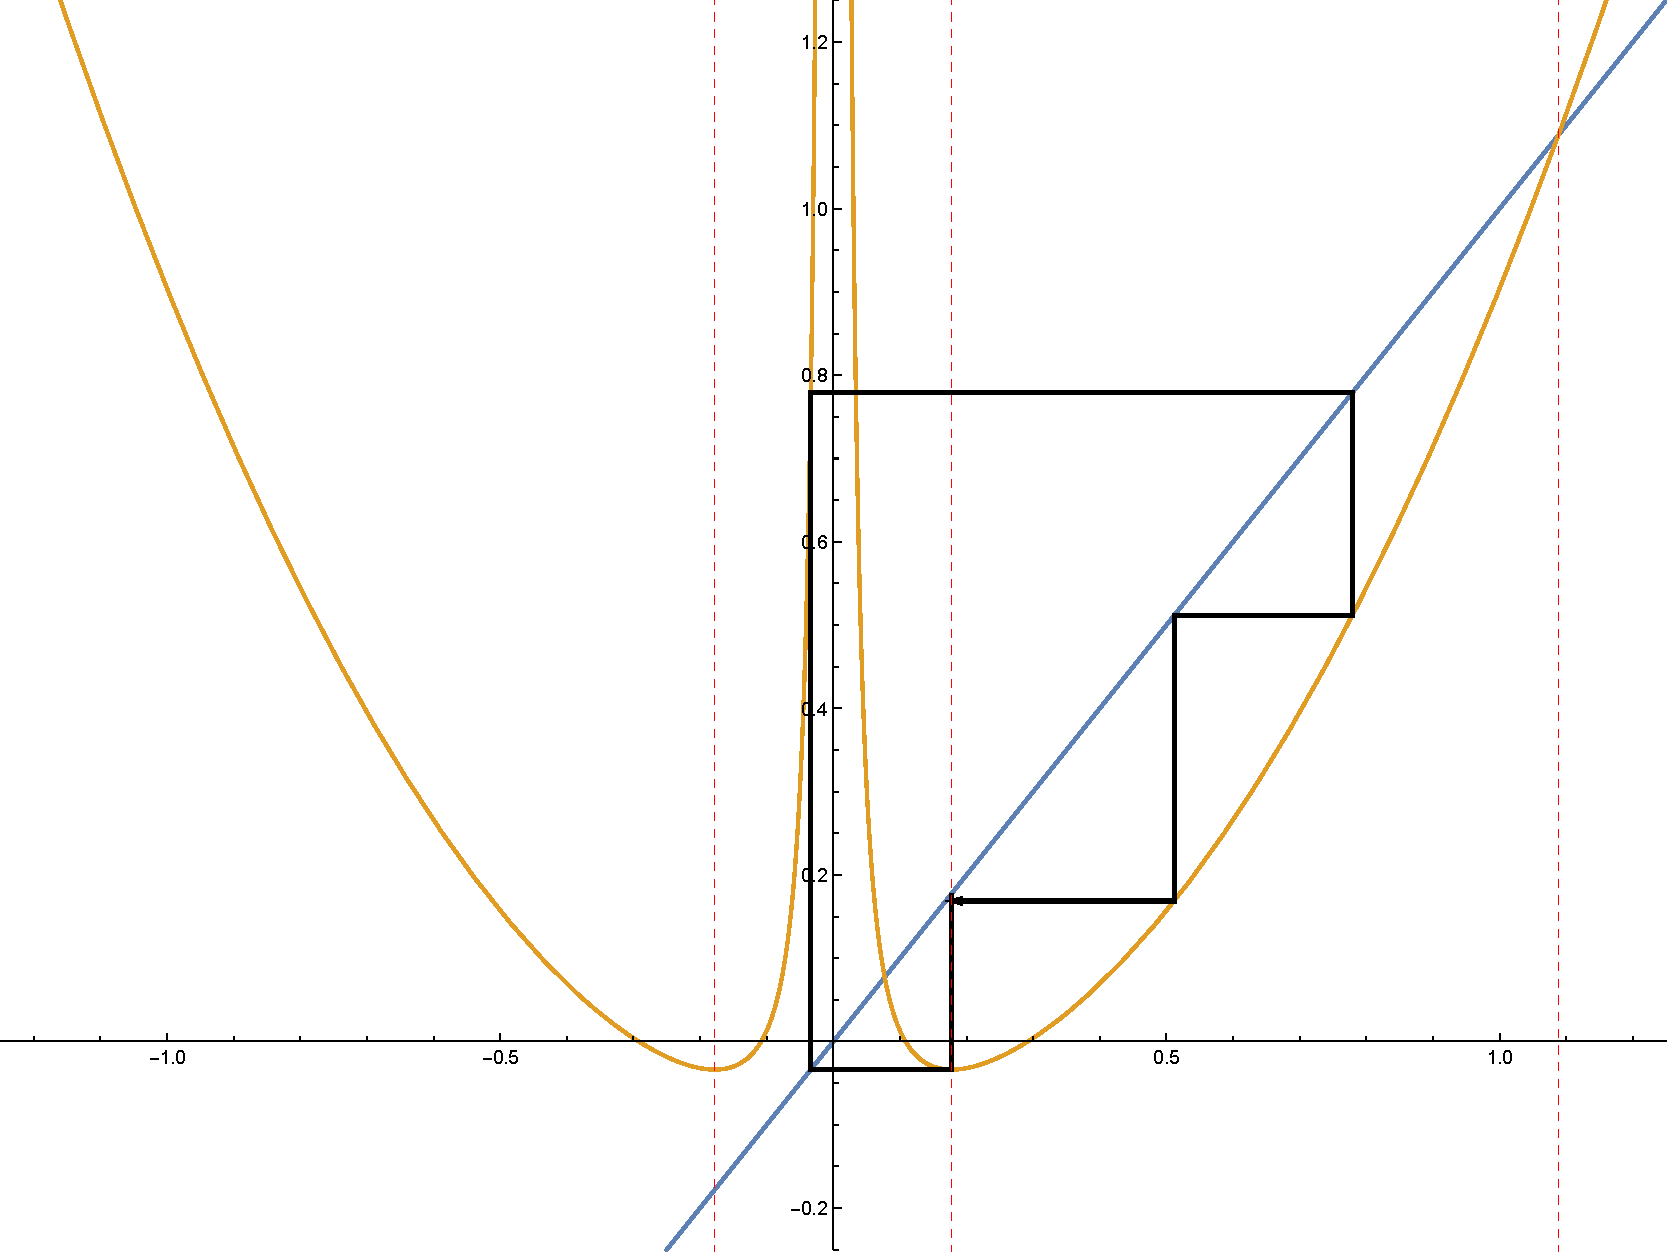
\includegraphics[width=\textwidth]{./img/CrFFC}
		% 		\caption{Seventh iterate of $f_c (C)$ added along with the parameter value of its prezero orbit}
		% 		\label{fig:cplot6S}
		% \end{subfigure}
		 %add desired spacing between images, e. g. ~, \quad, \qquad, \hfill etc.
		  % (or a blank line to force the subfigure onto a new line)
		\caption{Graphical iteration showing the accumulation of periodic, prefixed, and prezero orbits as $c$ approaches $\pl$ (depicted in 3.11 (k)) from the right and the accumulation of periodic, and prezero orbits as $c$ approaches $\pr$ (depicted in 3.10 (e))  from the left}\label{fig:giters}
\end{figure}

\begin{figure}[ht]
		\centering
		\begin{subfigure}[b]{0.3\textwidth}
				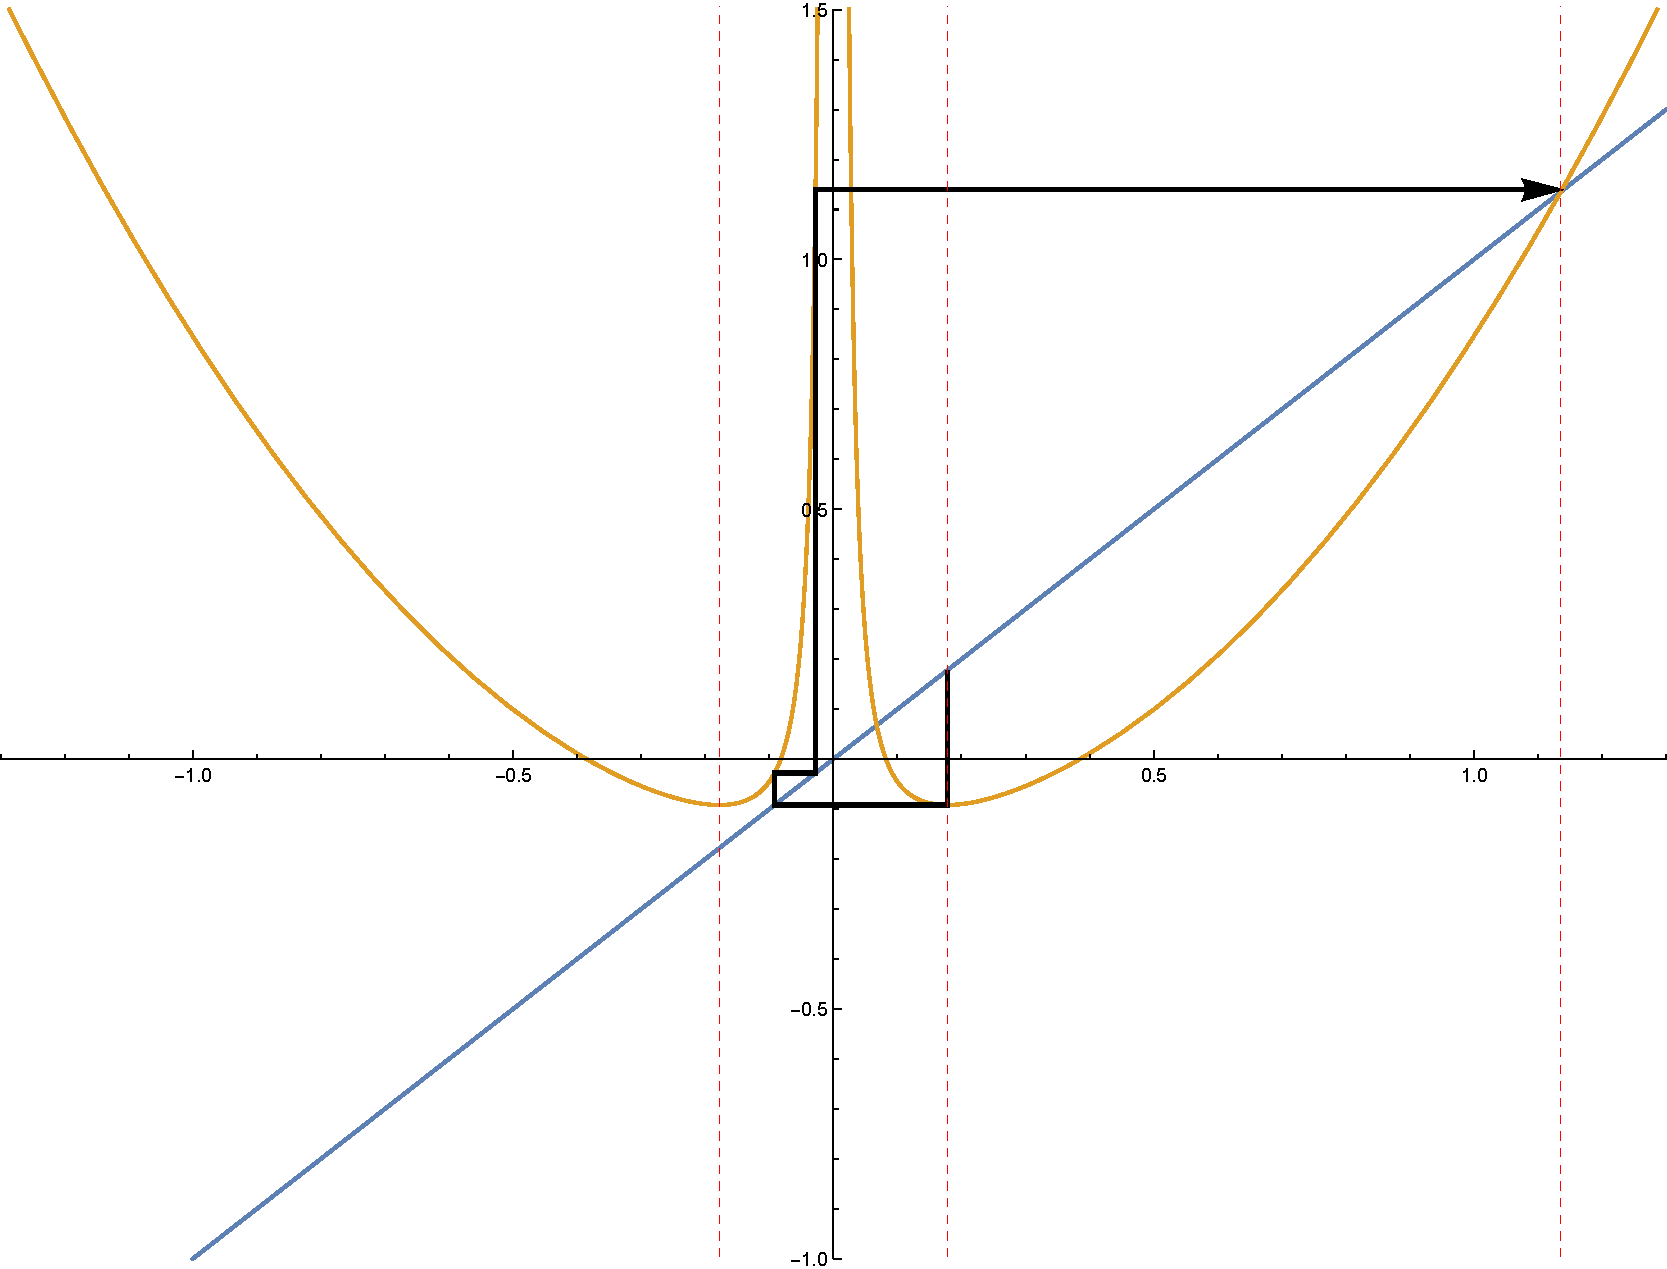
\includegraphics[width=\textwidth]{./img/plot-0155}
				\caption{$c \approx -.155 \approx h_3^{CrrP_c}$}
		\end{subfigure}
		\begin{subfigure}[b]{0.3\textwidth}
				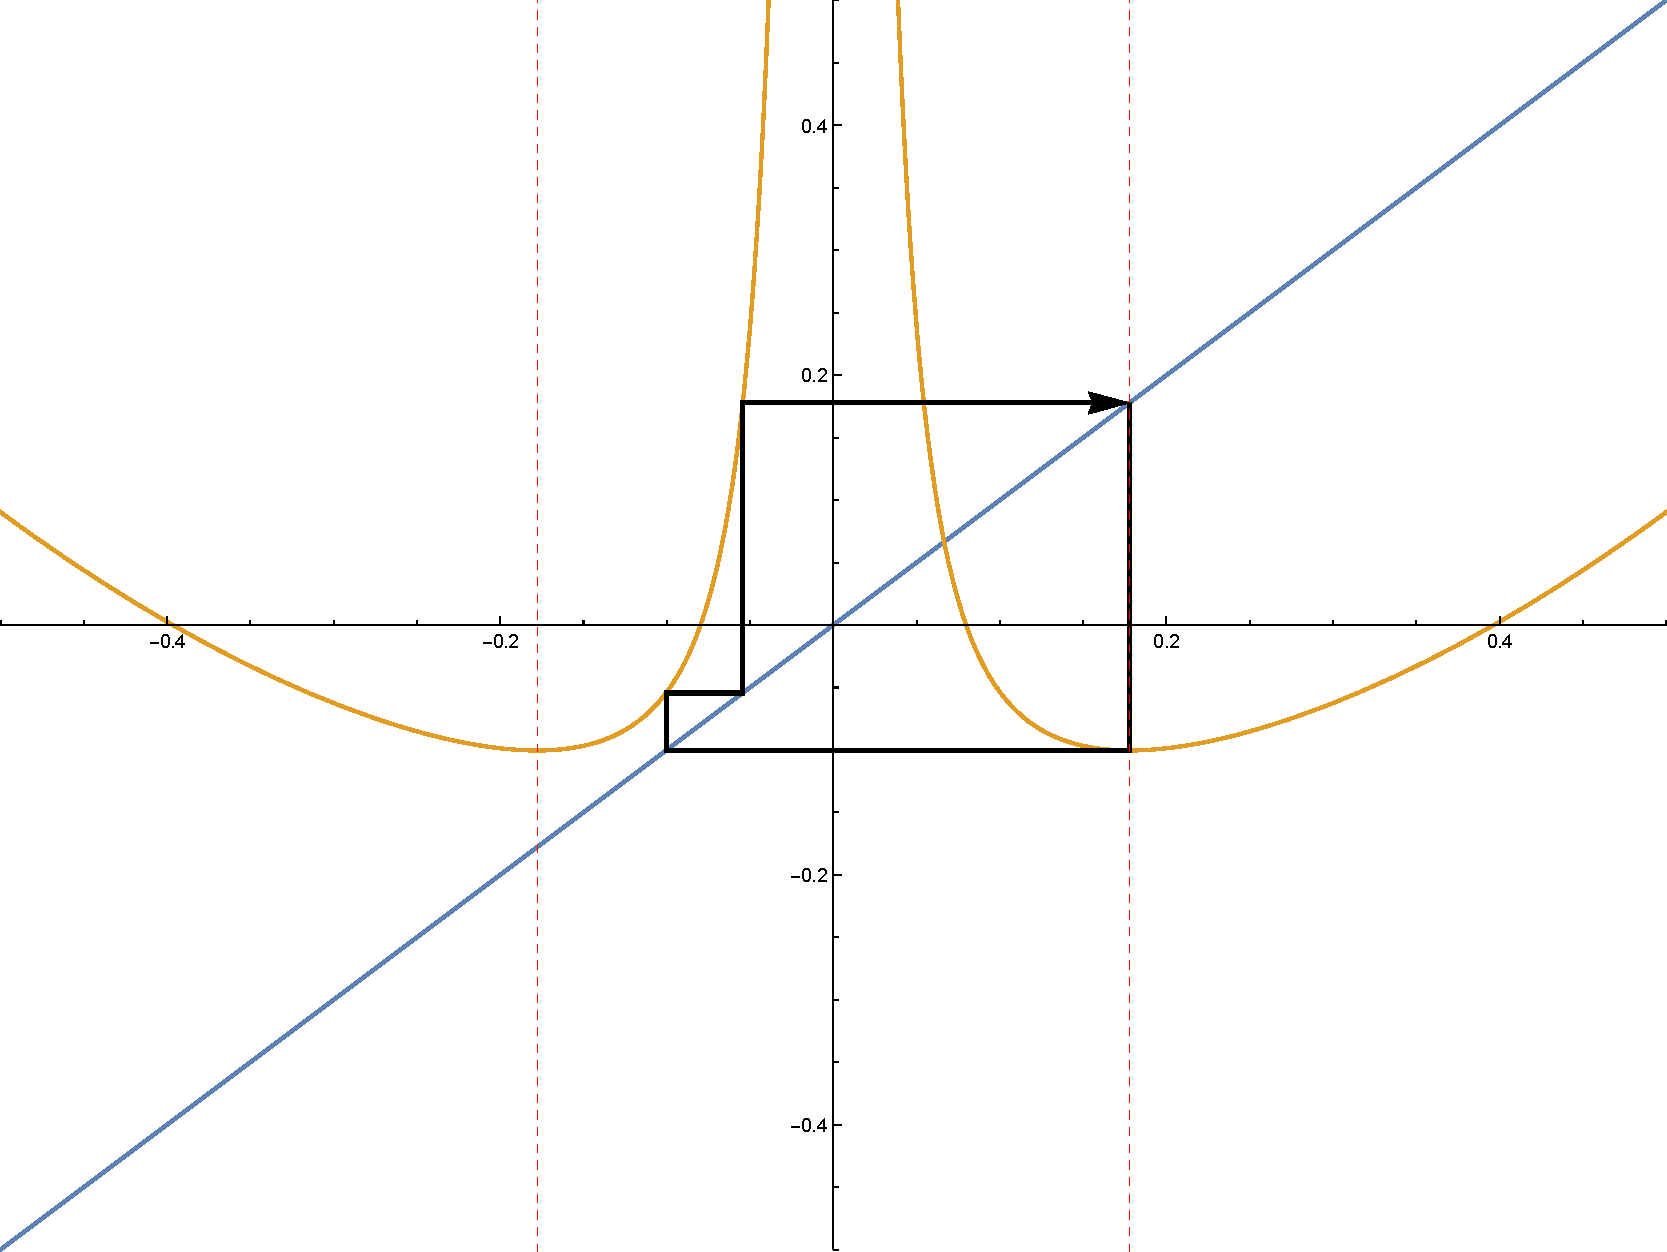
\includegraphics[width=\textwidth]{./img/plot-016364}
				\caption{$c \approx - .16364 \approx p_3^{CrrC}$}
		\end{subfigure}
		\begin{subfigure}[b]{0.3\textwidth}
				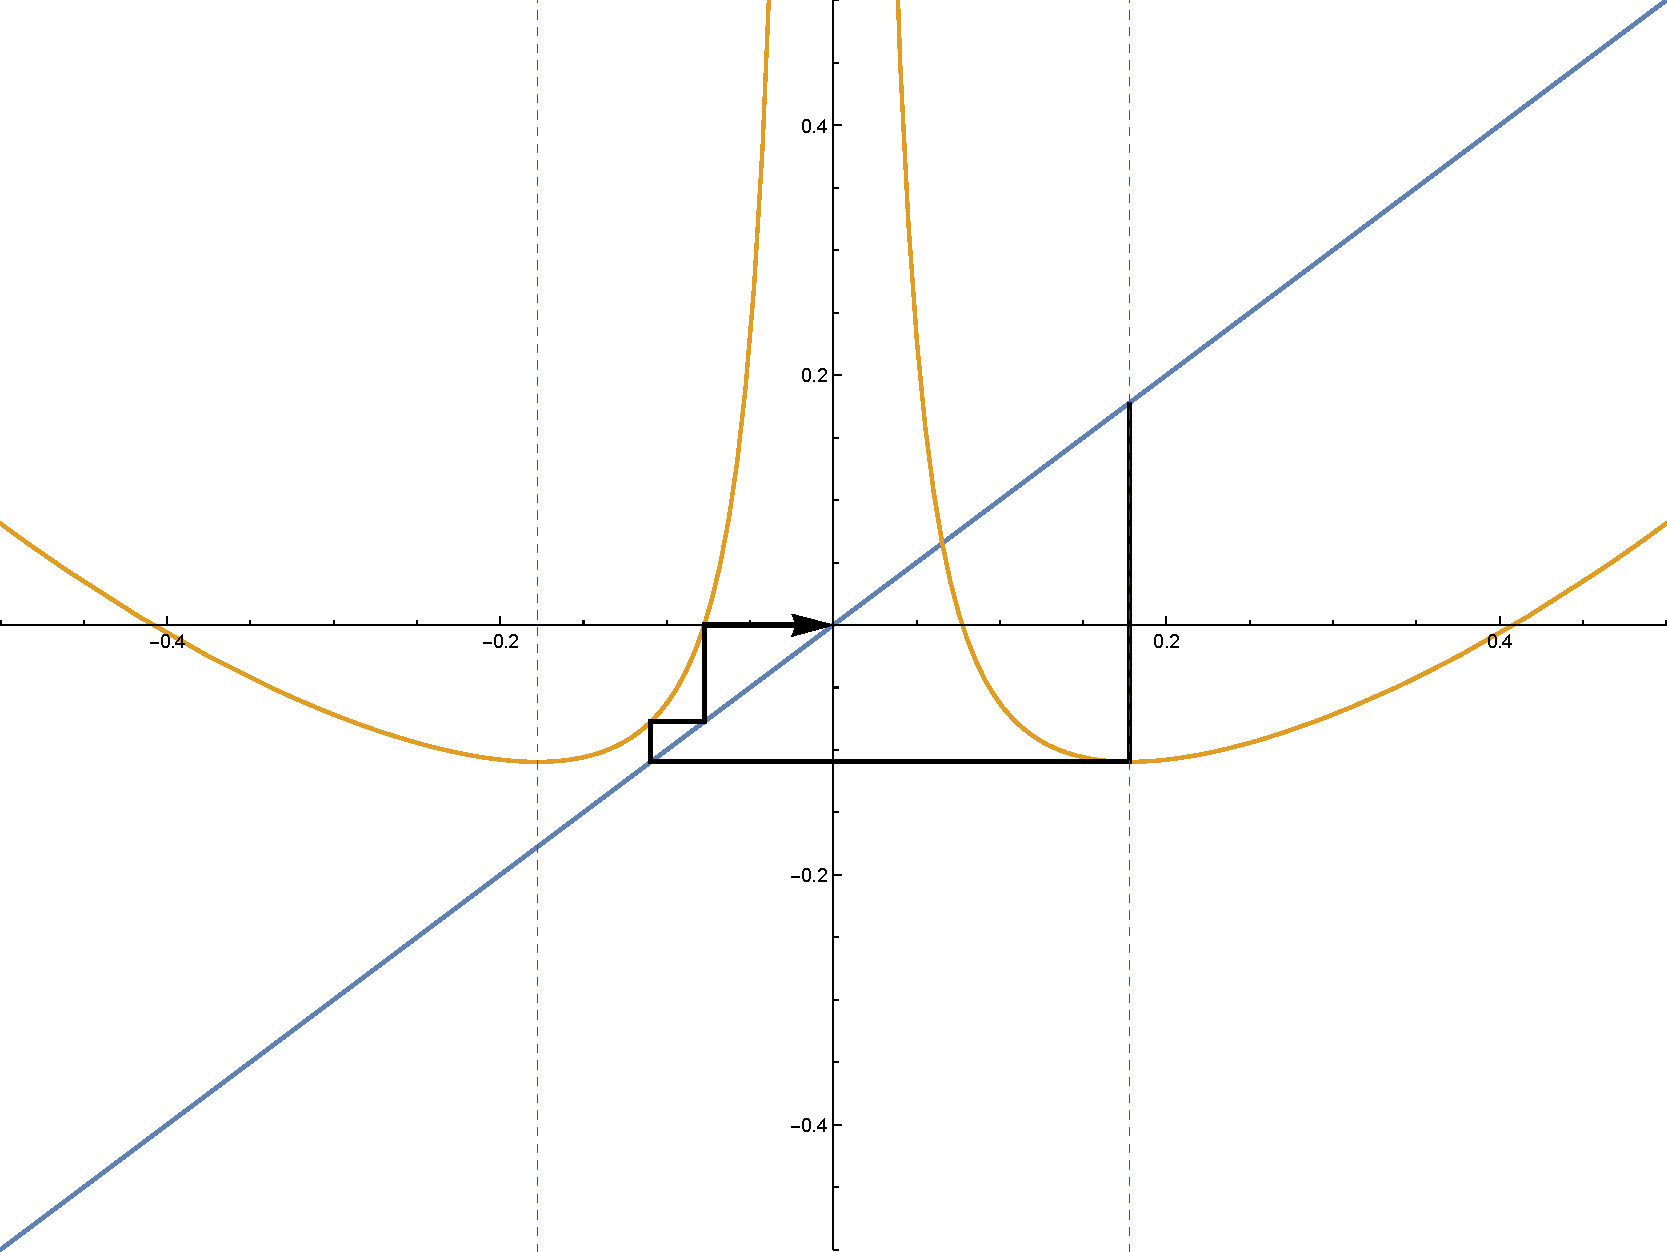
\includegraphics[width=\textwidth]{./img/plot-017278}
				\caption{$c \approx -.17278 \approx z_3^{Crr0}$}
		\end{subfigure}

		\begin{subfigure}[b]{0.3\textwidth}
				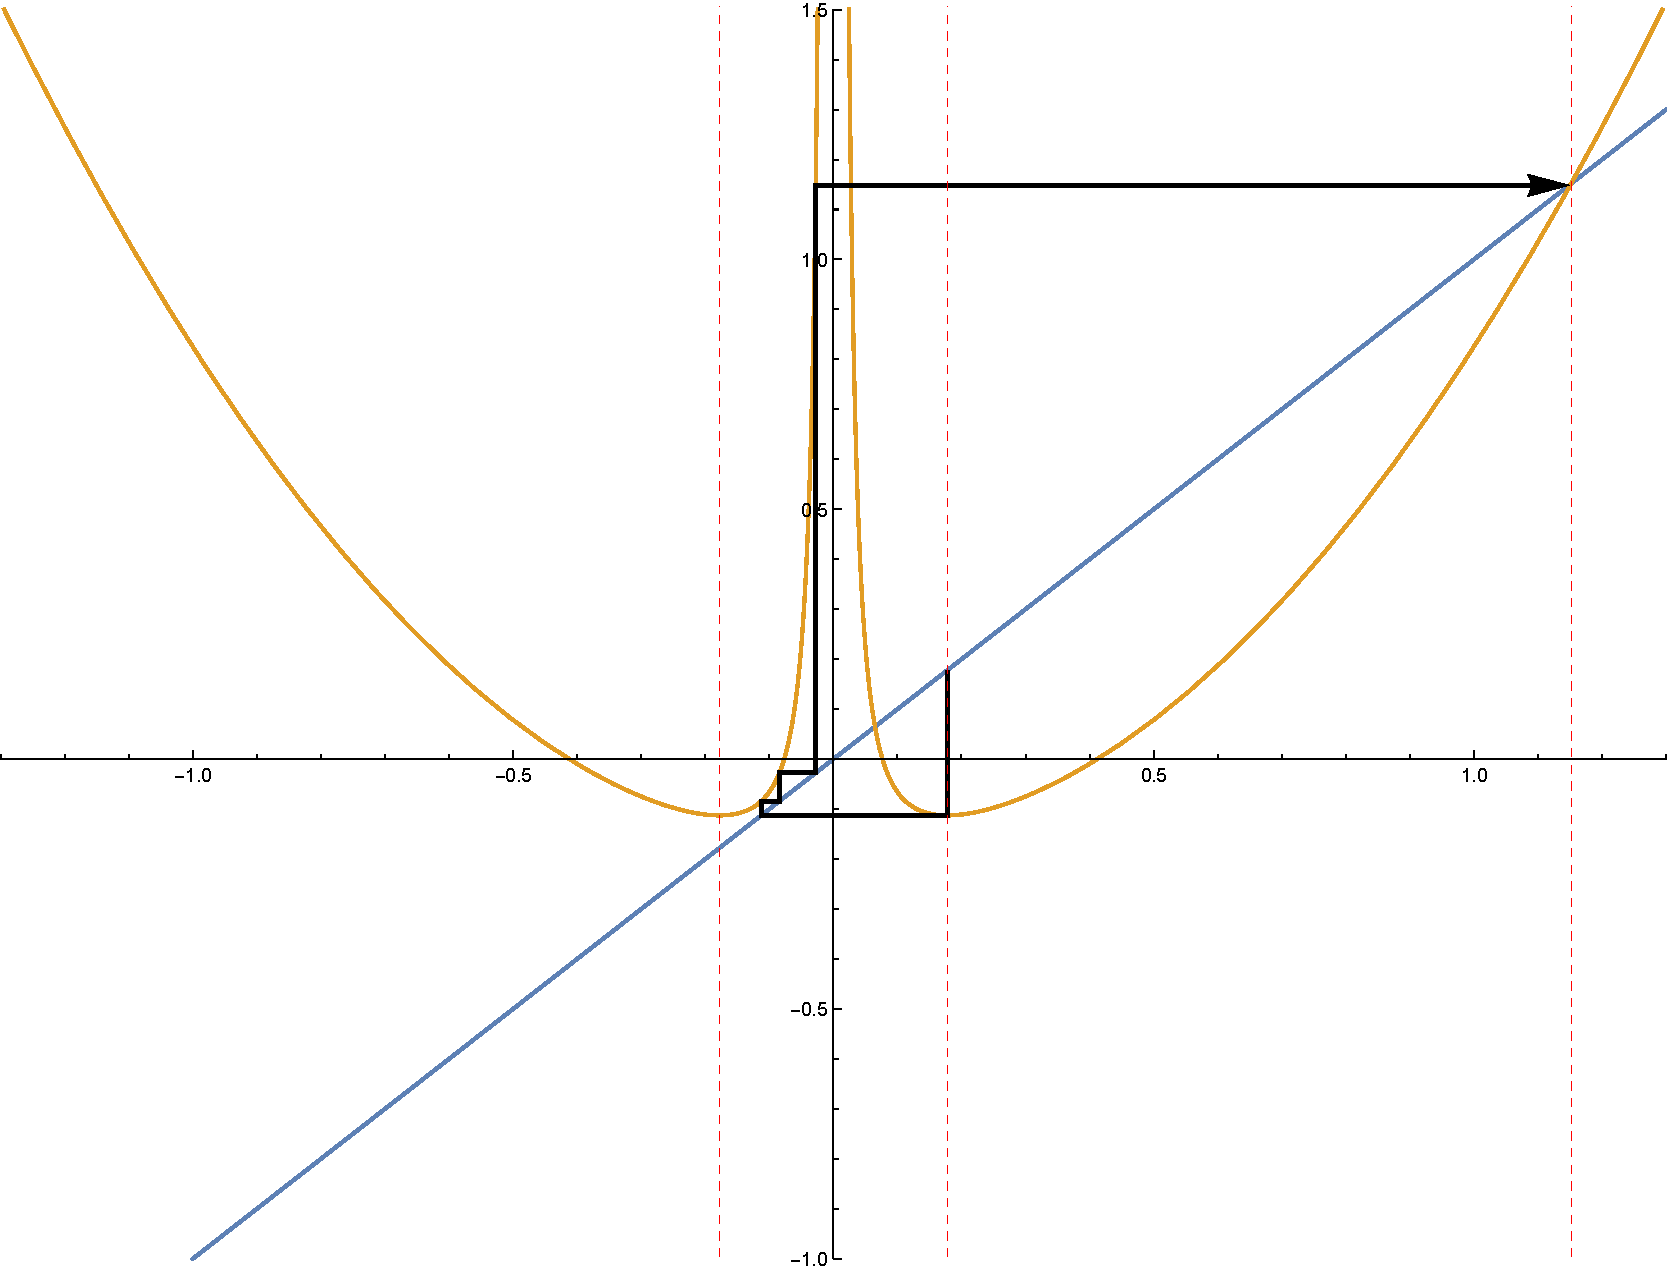
\includegraphics[width=\textwidth]{./img/plot-017578}
				\caption{$c \approx -.17578 \approx h_4^{CrrrP_c}$}
		\end{subfigure}
		\begin{subfigure}[b]{0.3\textwidth}
				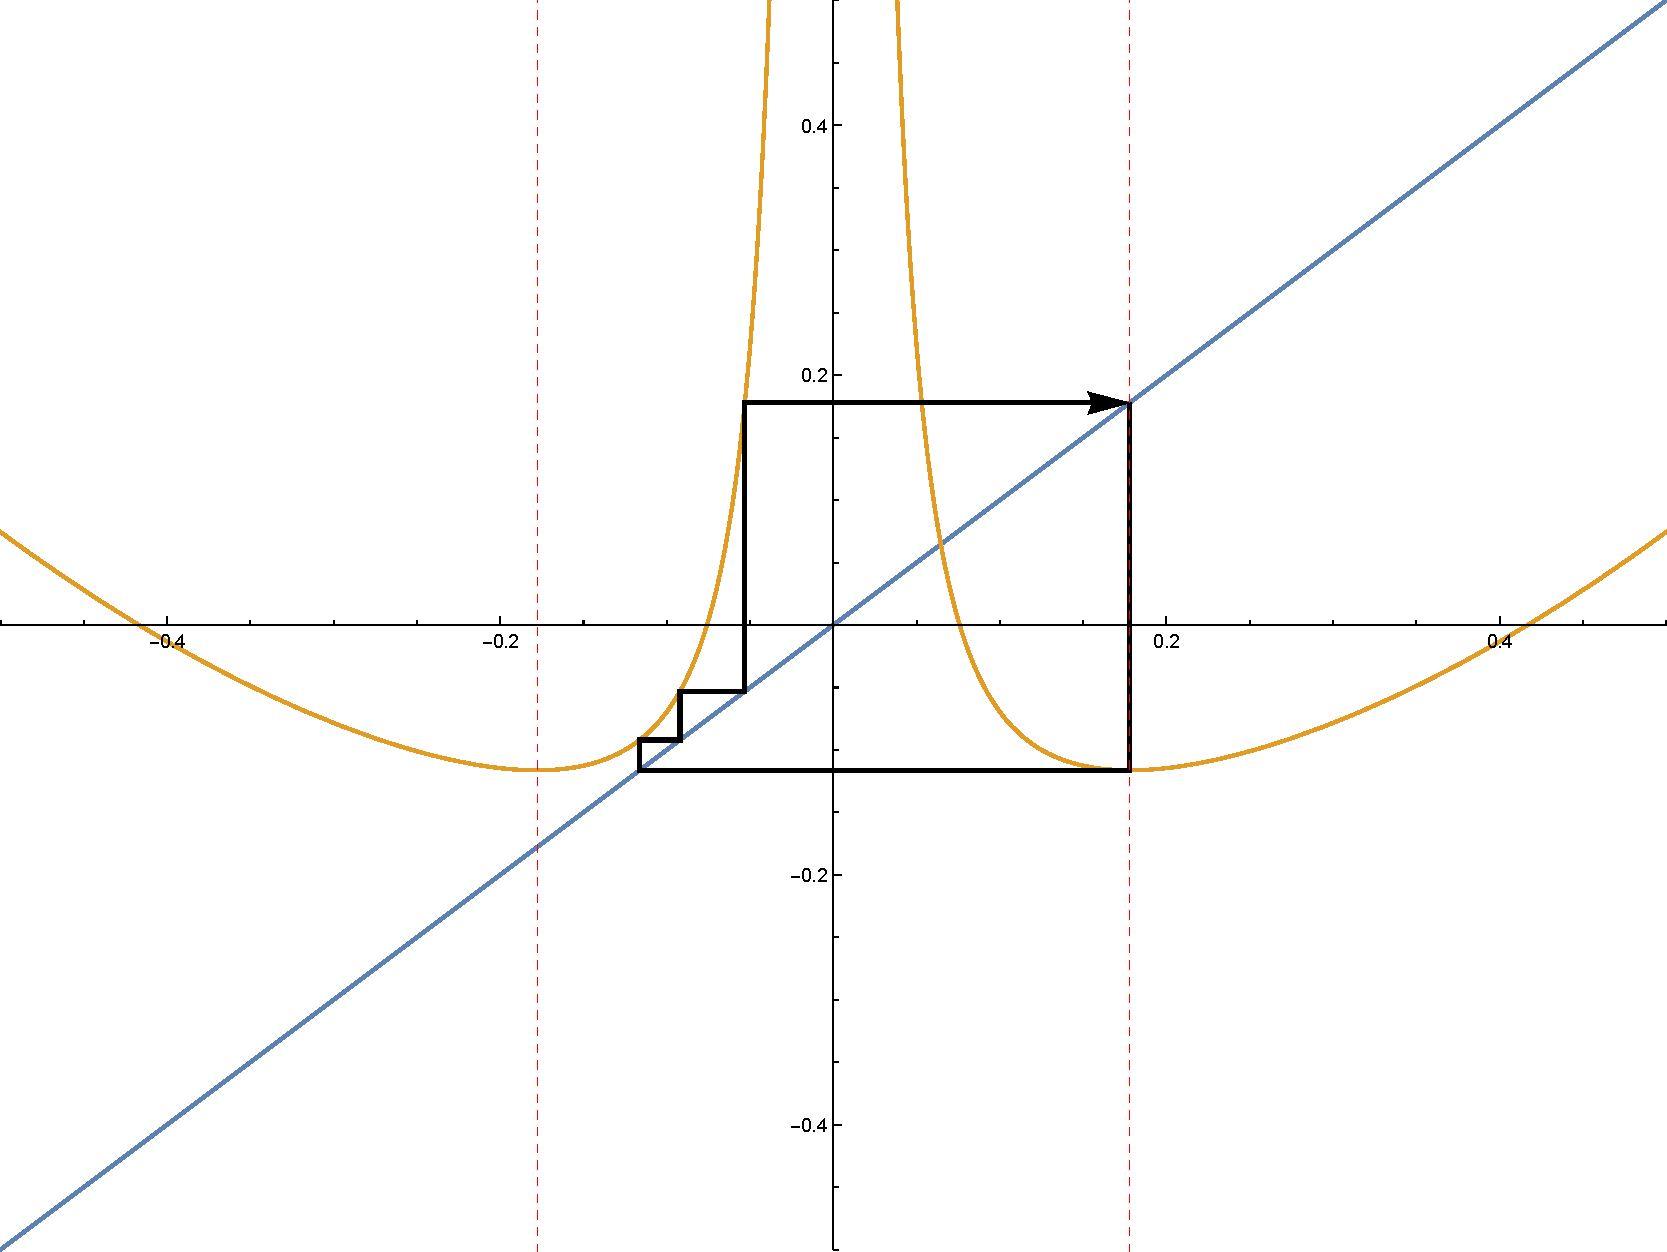
\includegraphics[width=\textwidth]{./img/plot-017954}
				\caption{$c \approx - .17954 \approx p_4^{CrrrC}$}
		\end{subfigure}
		\begin{subfigure}[b]{0.3\textwidth}
				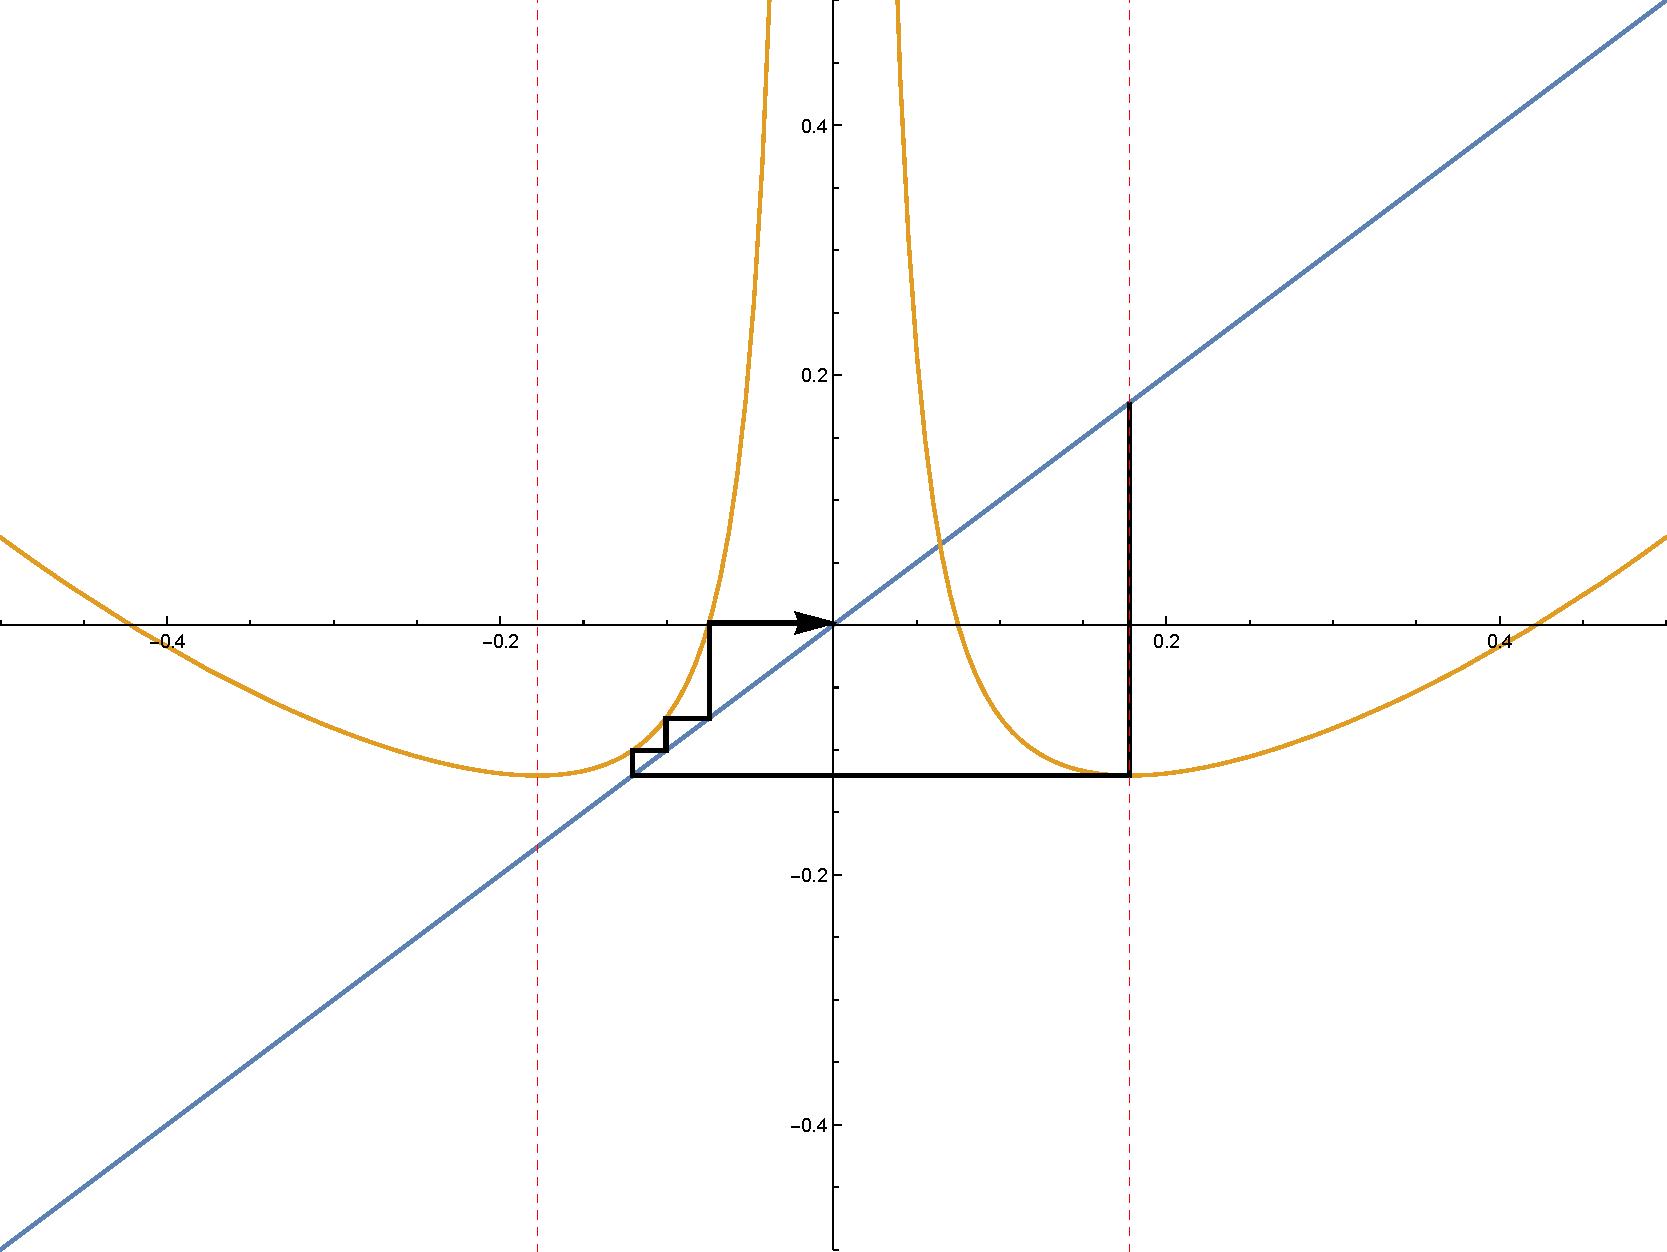
\includegraphics[width=\textwidth]{./img/plot-018378}
				\caption{$c \approx -.18378 \approx z_4^{Crrr0}$}
		\end{subfigure}

		\begin{subfigure}[b]{0.3\textwidth}
				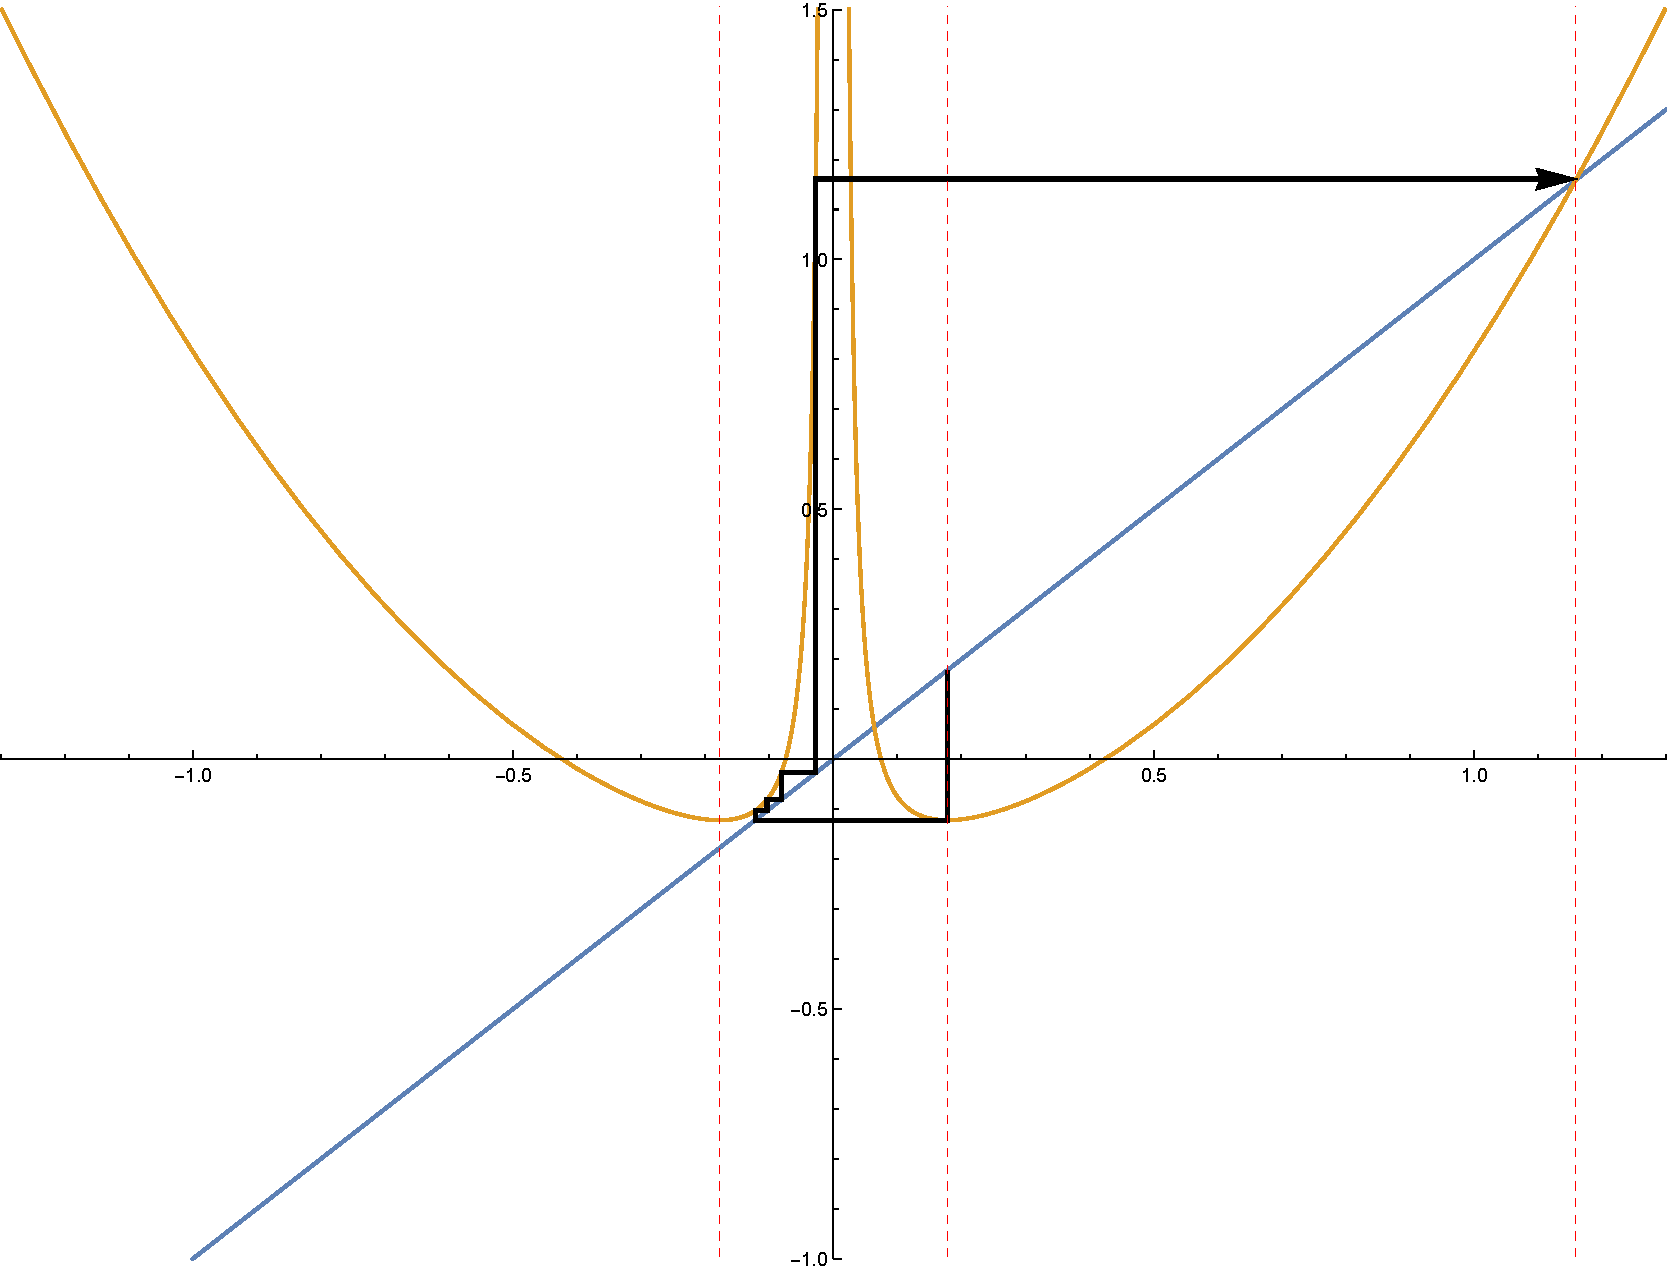
\includegraphics[width=\textwidth]{./img/plot-018539}
				\caption{$c \approx -.18539 \approx h_5^{CrrrrP_c}$}
		\end{subfigure}
		\begin{subfigure}[b]{0.3\textwidth}
				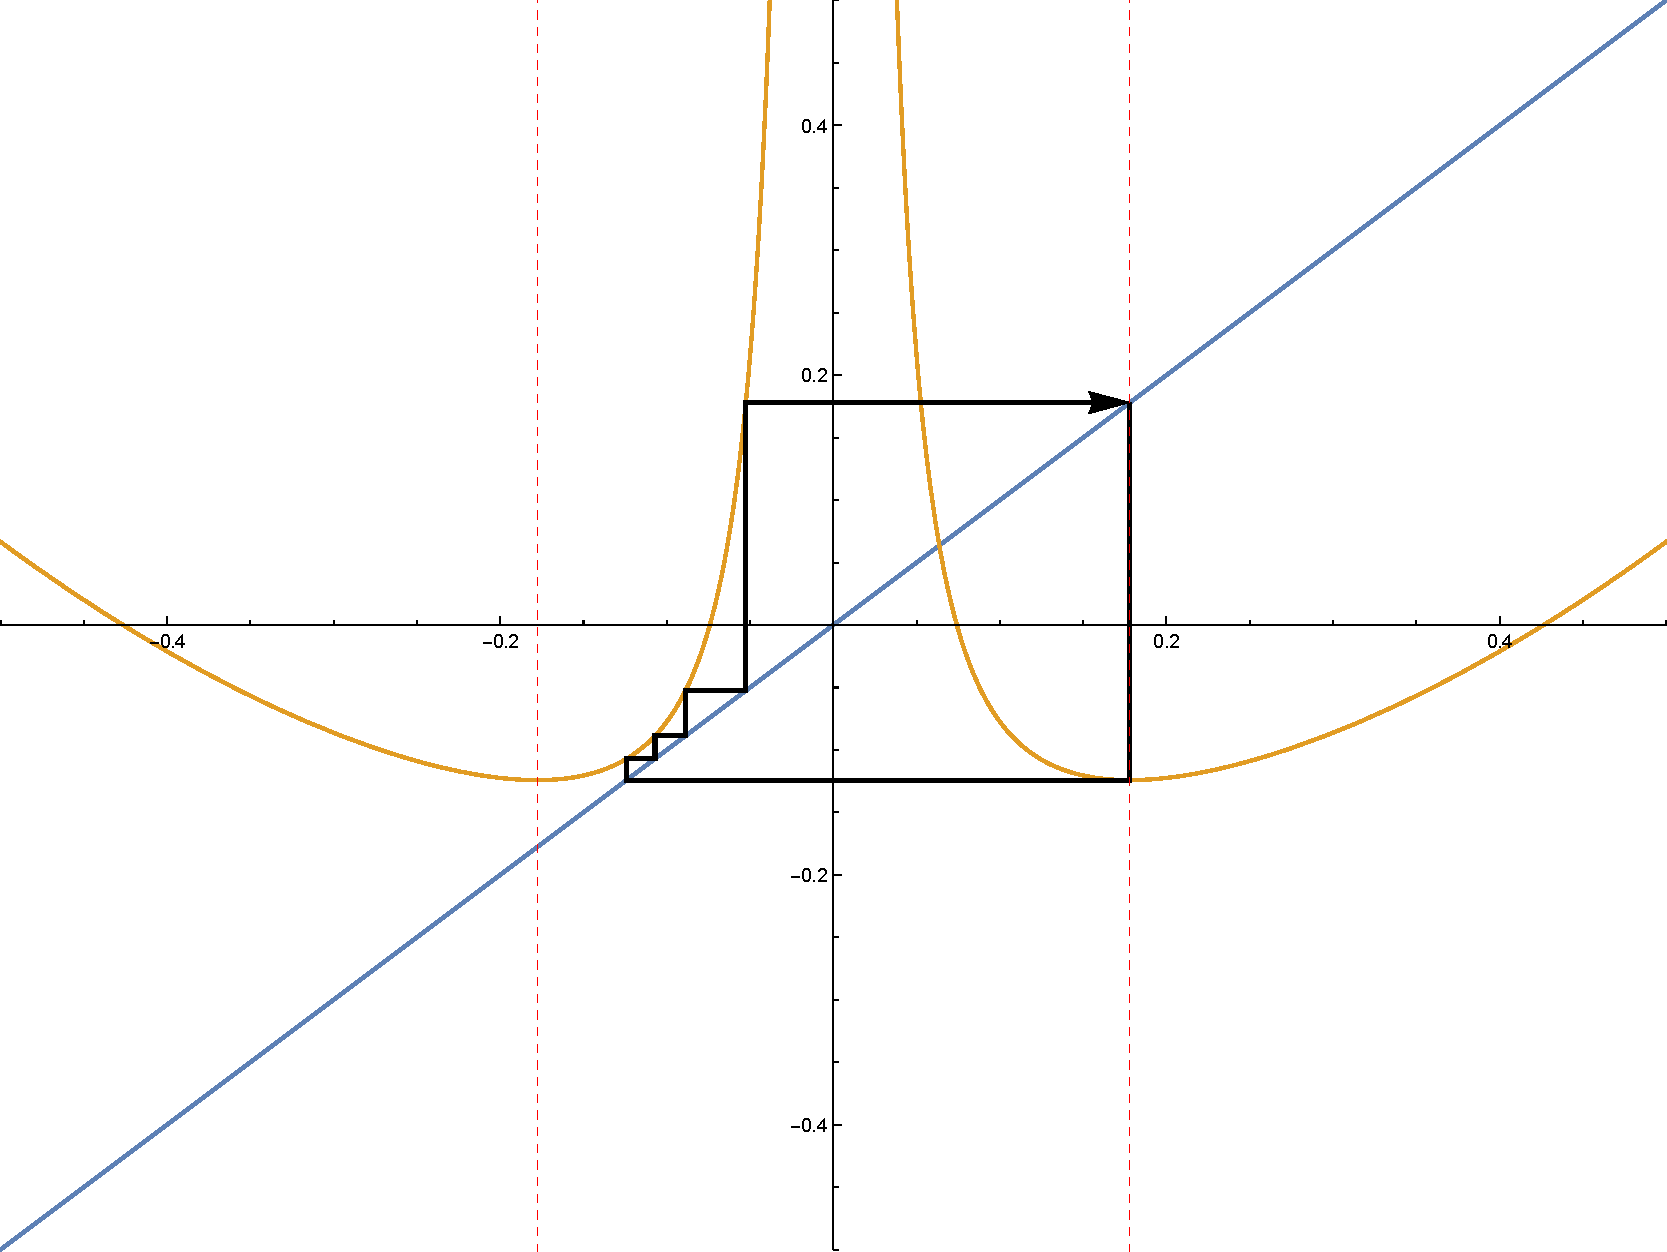
\includegraphics[width=\textwidth]{./img/plot-018739}
				\caption{$c \approx - .18739\approx p_5^{CrrrrC}$}
		\end{subfigure}
		\begin{subfigure}[b]{0.3\textwidth}
				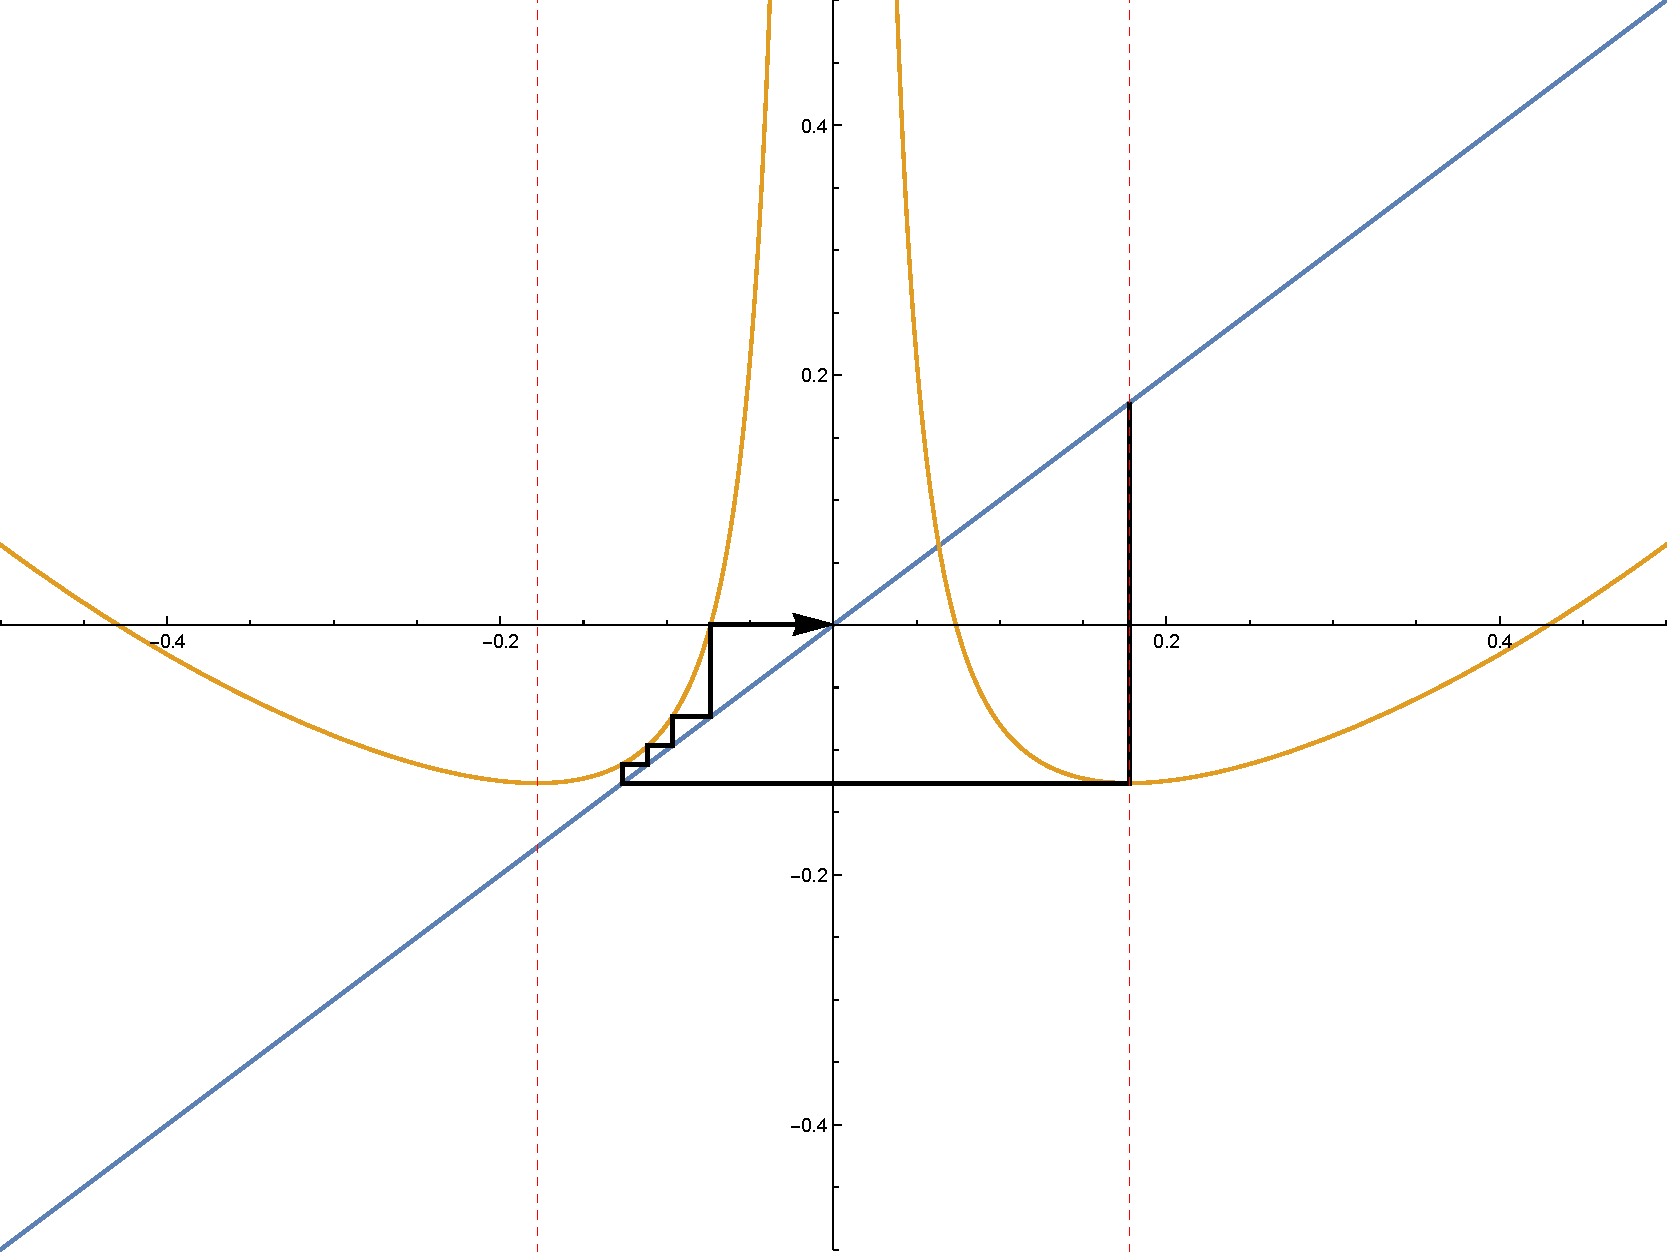
\includegraphics[width=\textwidth]{./img/plot-018979}
				\caption{$c \approx - .18979 \approx z_5^{Crrrr0}$}
		\end{subfigure}

		\begin{subfigure}[b]{0.3\textwidth}
				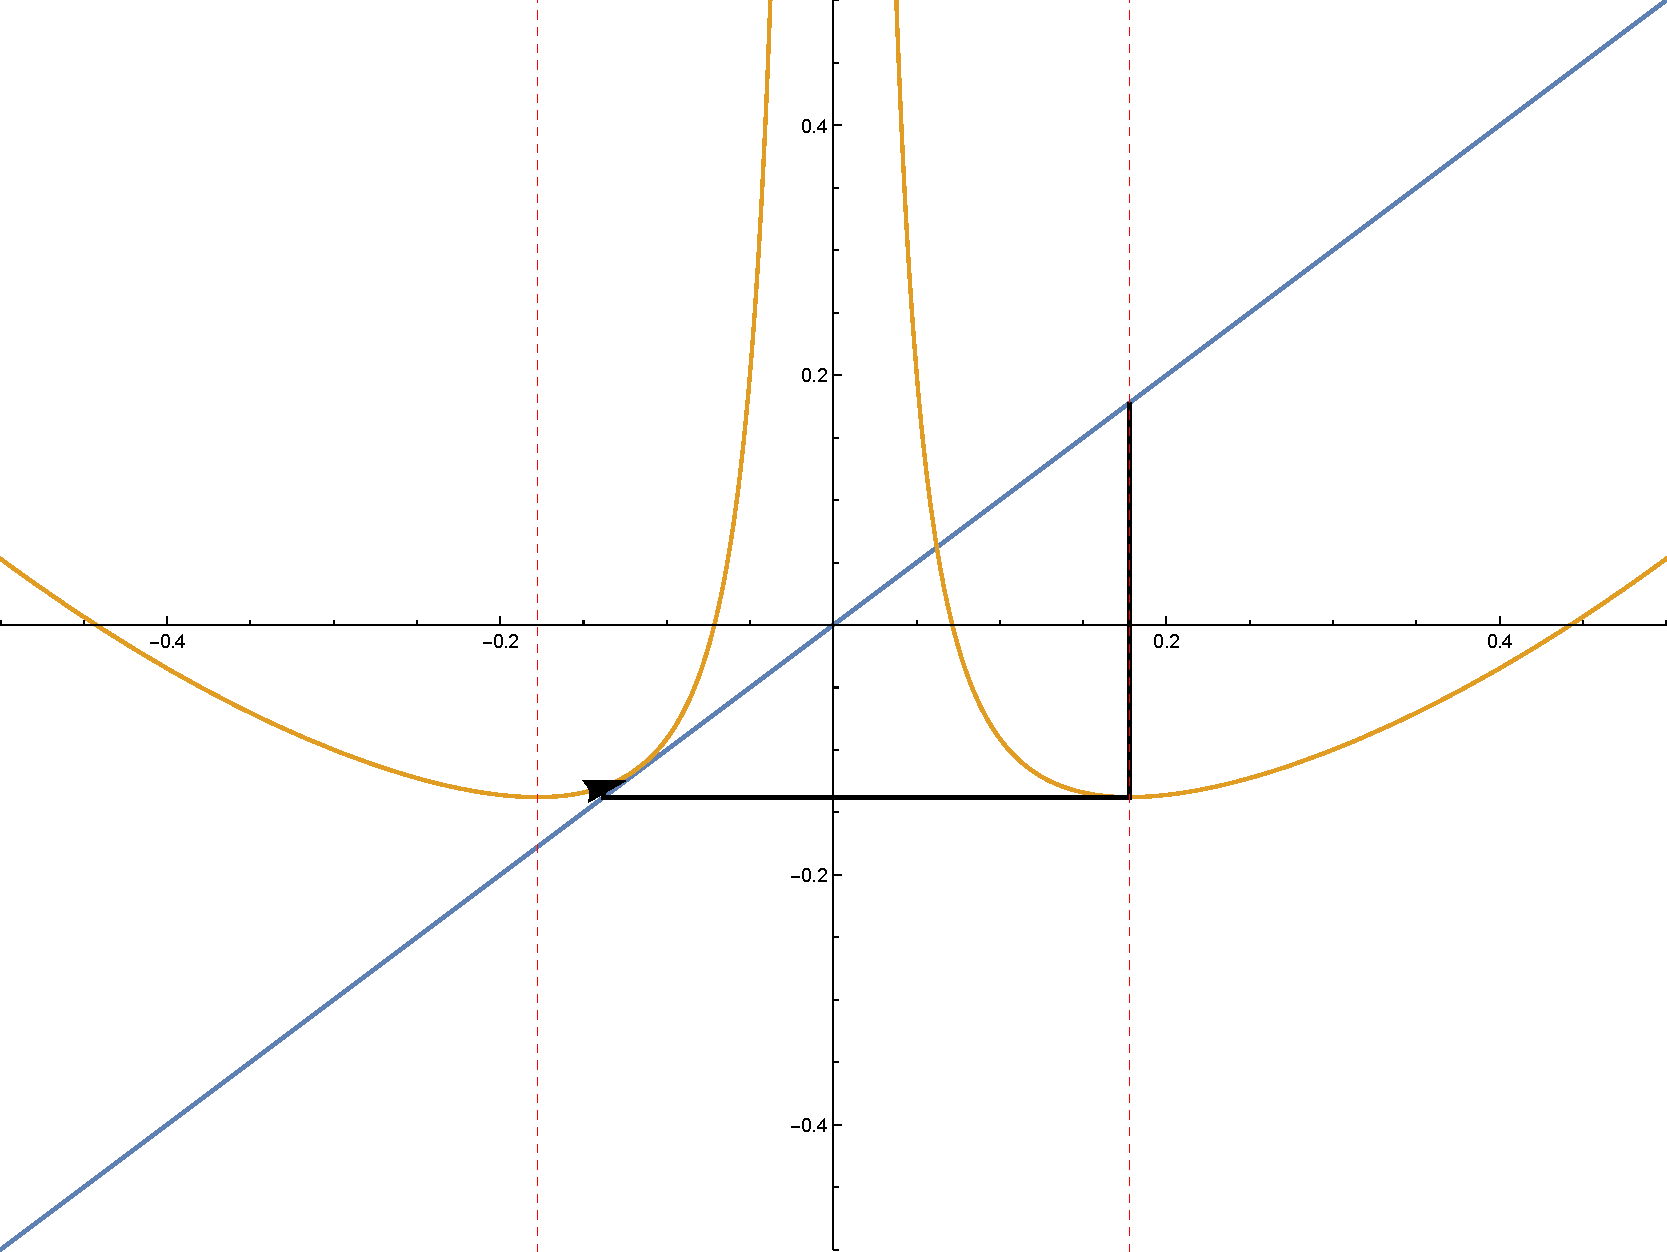
\includegraphics[width=\textwidth]{./img/plot-0201}
				\caption{$c \approx - .201\approx s_1^l$}
		\end{subfigure}
		\begin{subfigure}[b]{0.3\textwidth}
				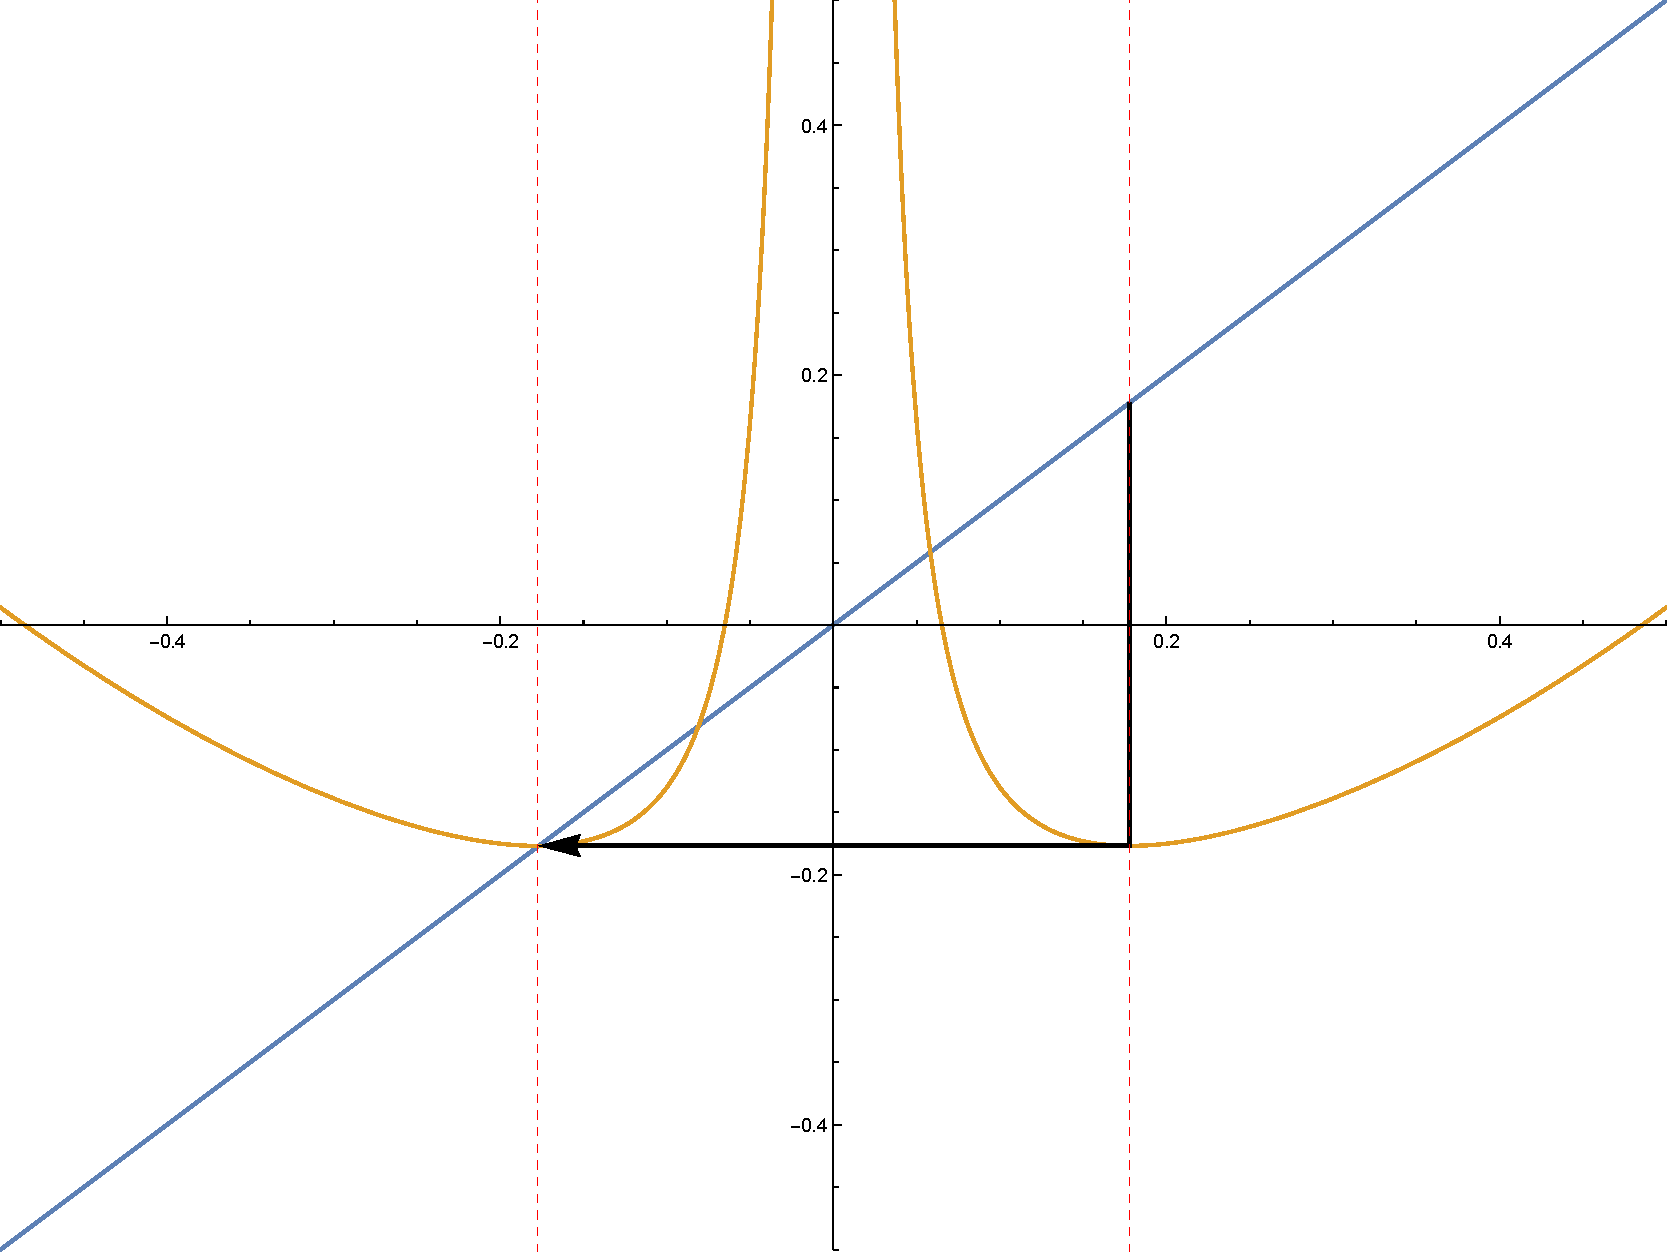
\includegraphics[width=\textwidth]{./img/plot-024}
				\caption{$c \approx -.24 \approx p_1^{-C}$}
		\end{subfigure}
		% \begin{subfigure}[b]{0.3\textwidth}
		% 		\includegraphics[width=\textwidth]{./img/plot-}
		% 		\caption{Seventh iterate of $f_c (C)$ added along with the parameter value of its prezero orbit}
		% 		\label{fig:cplot6S}
		% \end{subfigure}
		% \begin{subfigure}[b]{0.333\textwidth}
		% 		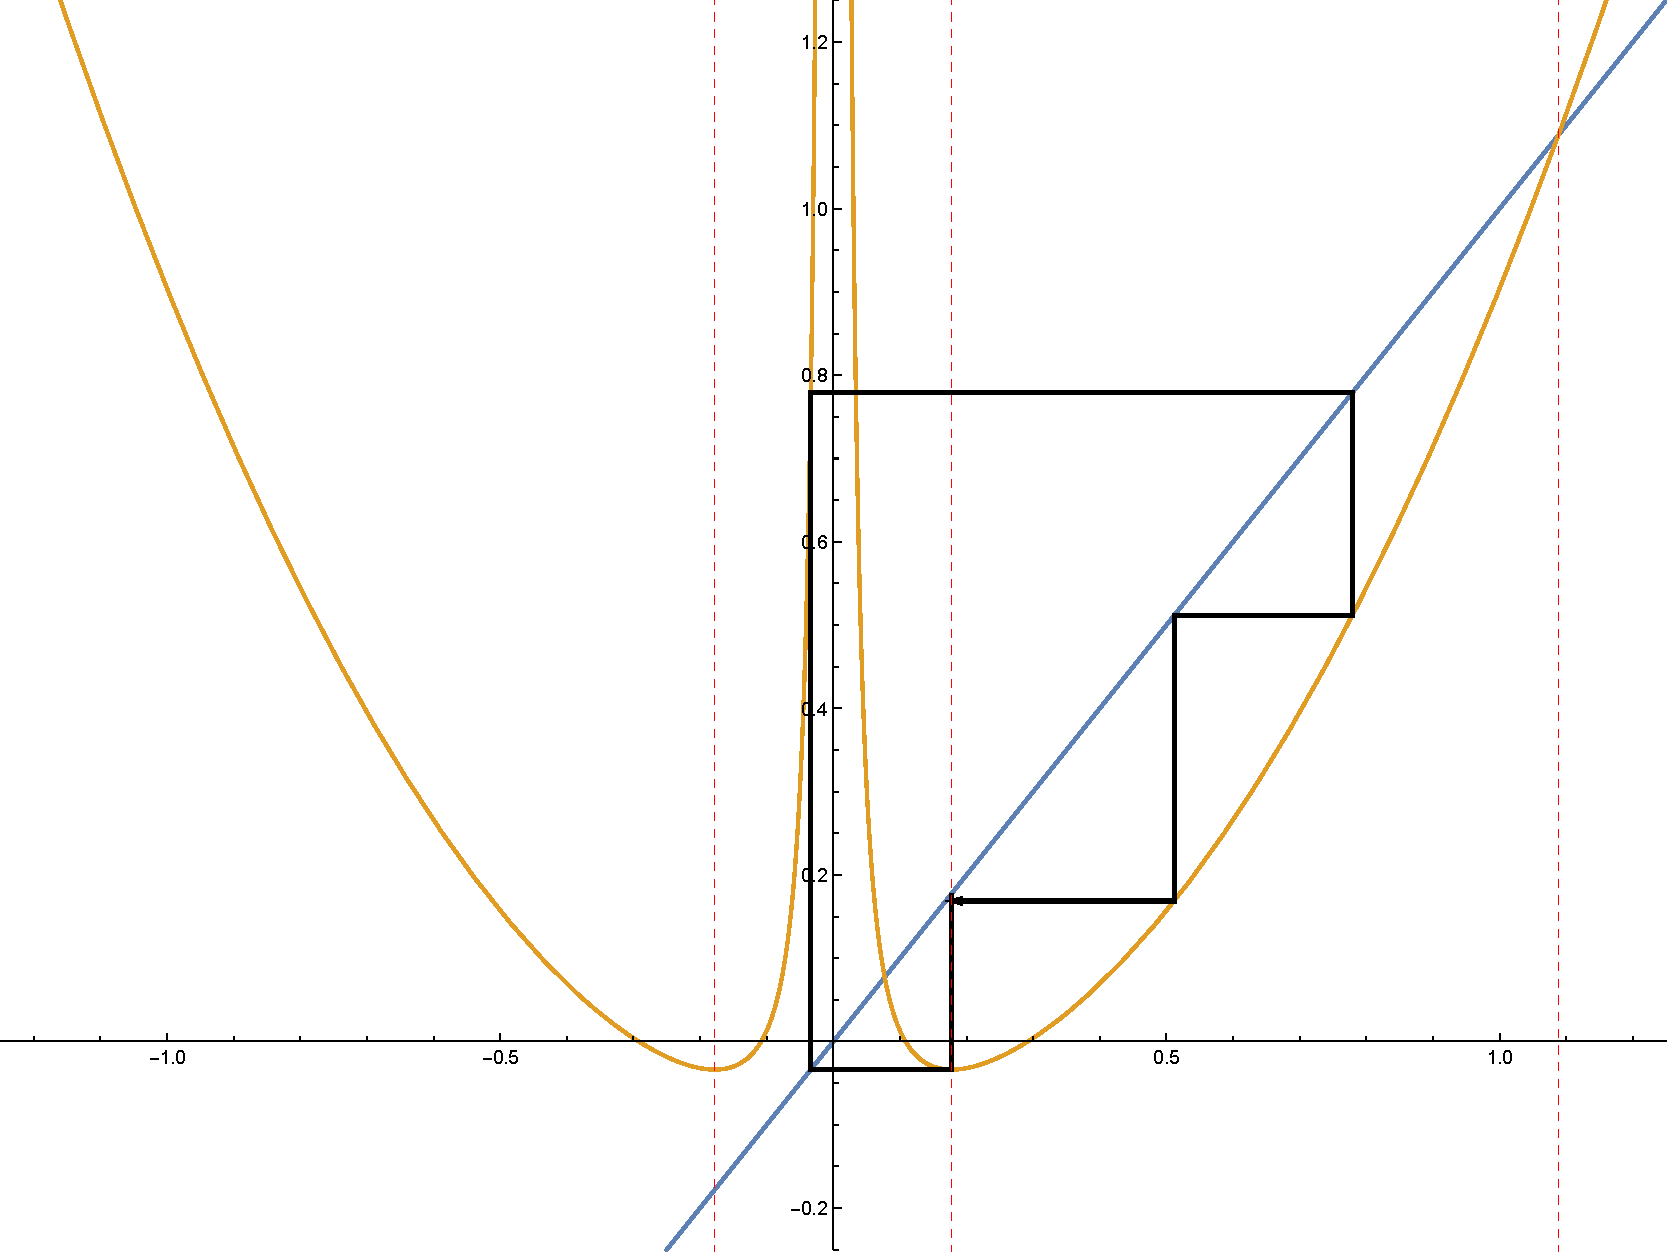
\includegraphics[width=\textwidth]{./img/CrFFC}
		% 		\caption{Seventh iterate of $f_c (C)$ added along with the parameter value of its prezero orbit}
		% 		\label{fig:cplot6S}
		% \end{subfigure}
		 %add desired spacing between images, e. g. ~, \quad, \qquad, \hfill etc.
		  % (or a blank line to force the subfigure onto a new line)
		\caption{Graphical iteration showing the accumulation of periodic, prefixed, and prezero orbits as $c$ approaches $\pl$ (depicted in 3.11 (k)) from the right and the accumulation of periodic, and prezero orbits as $c$ approaches $\pr$ (depicted in 3.10 (e))  from the left (continued)}\label{fig:giters2}
\end{figure}

\begin{figure}[ht]
		\centering
		\begin{subfigure}[b]{0.5\textwidth}
				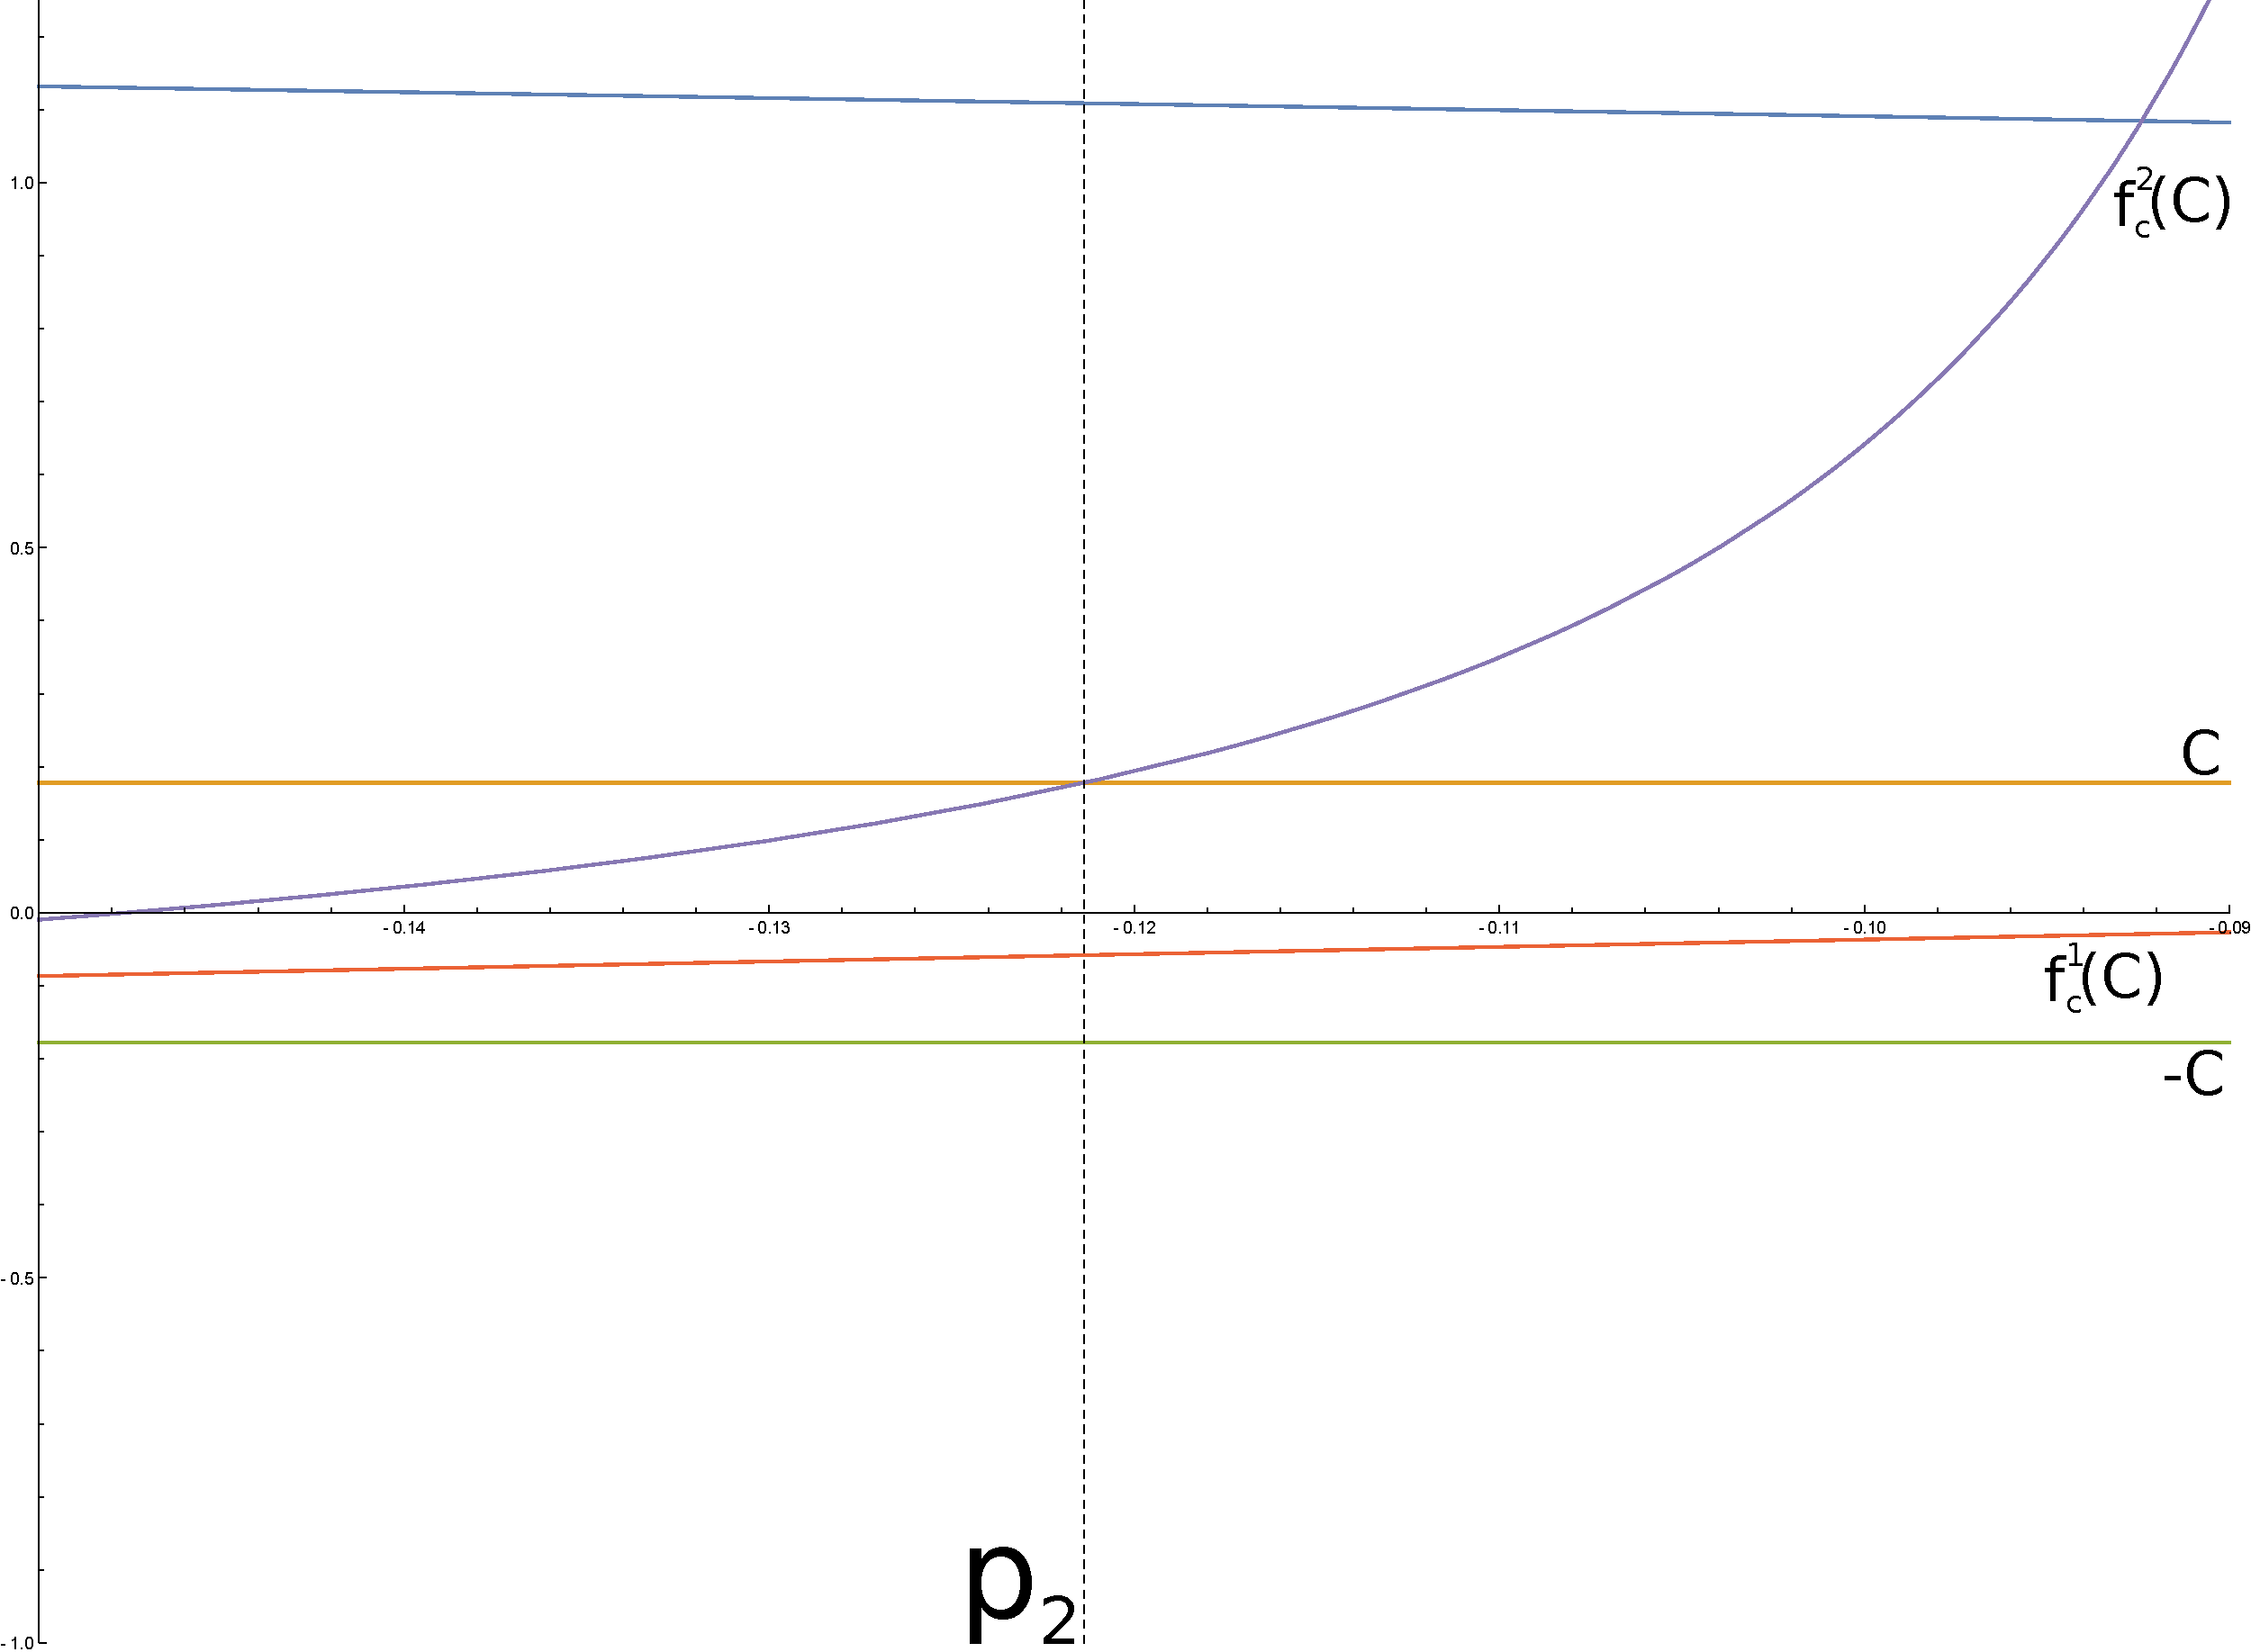
\includegraphics[width=\textwidth]{./img/cplot1H}
				\caption{$n = 2$}
				\label{fig:cplot1H}
		\end{subfigure}%
		~ %add desired spacing between images, e. g. ~, \quad, \qquad, \hfill etc.
		  % (or a blank line to force the subfigure onto a new line)
		\begin{subfigure}[b]{0.5\textwidth}
				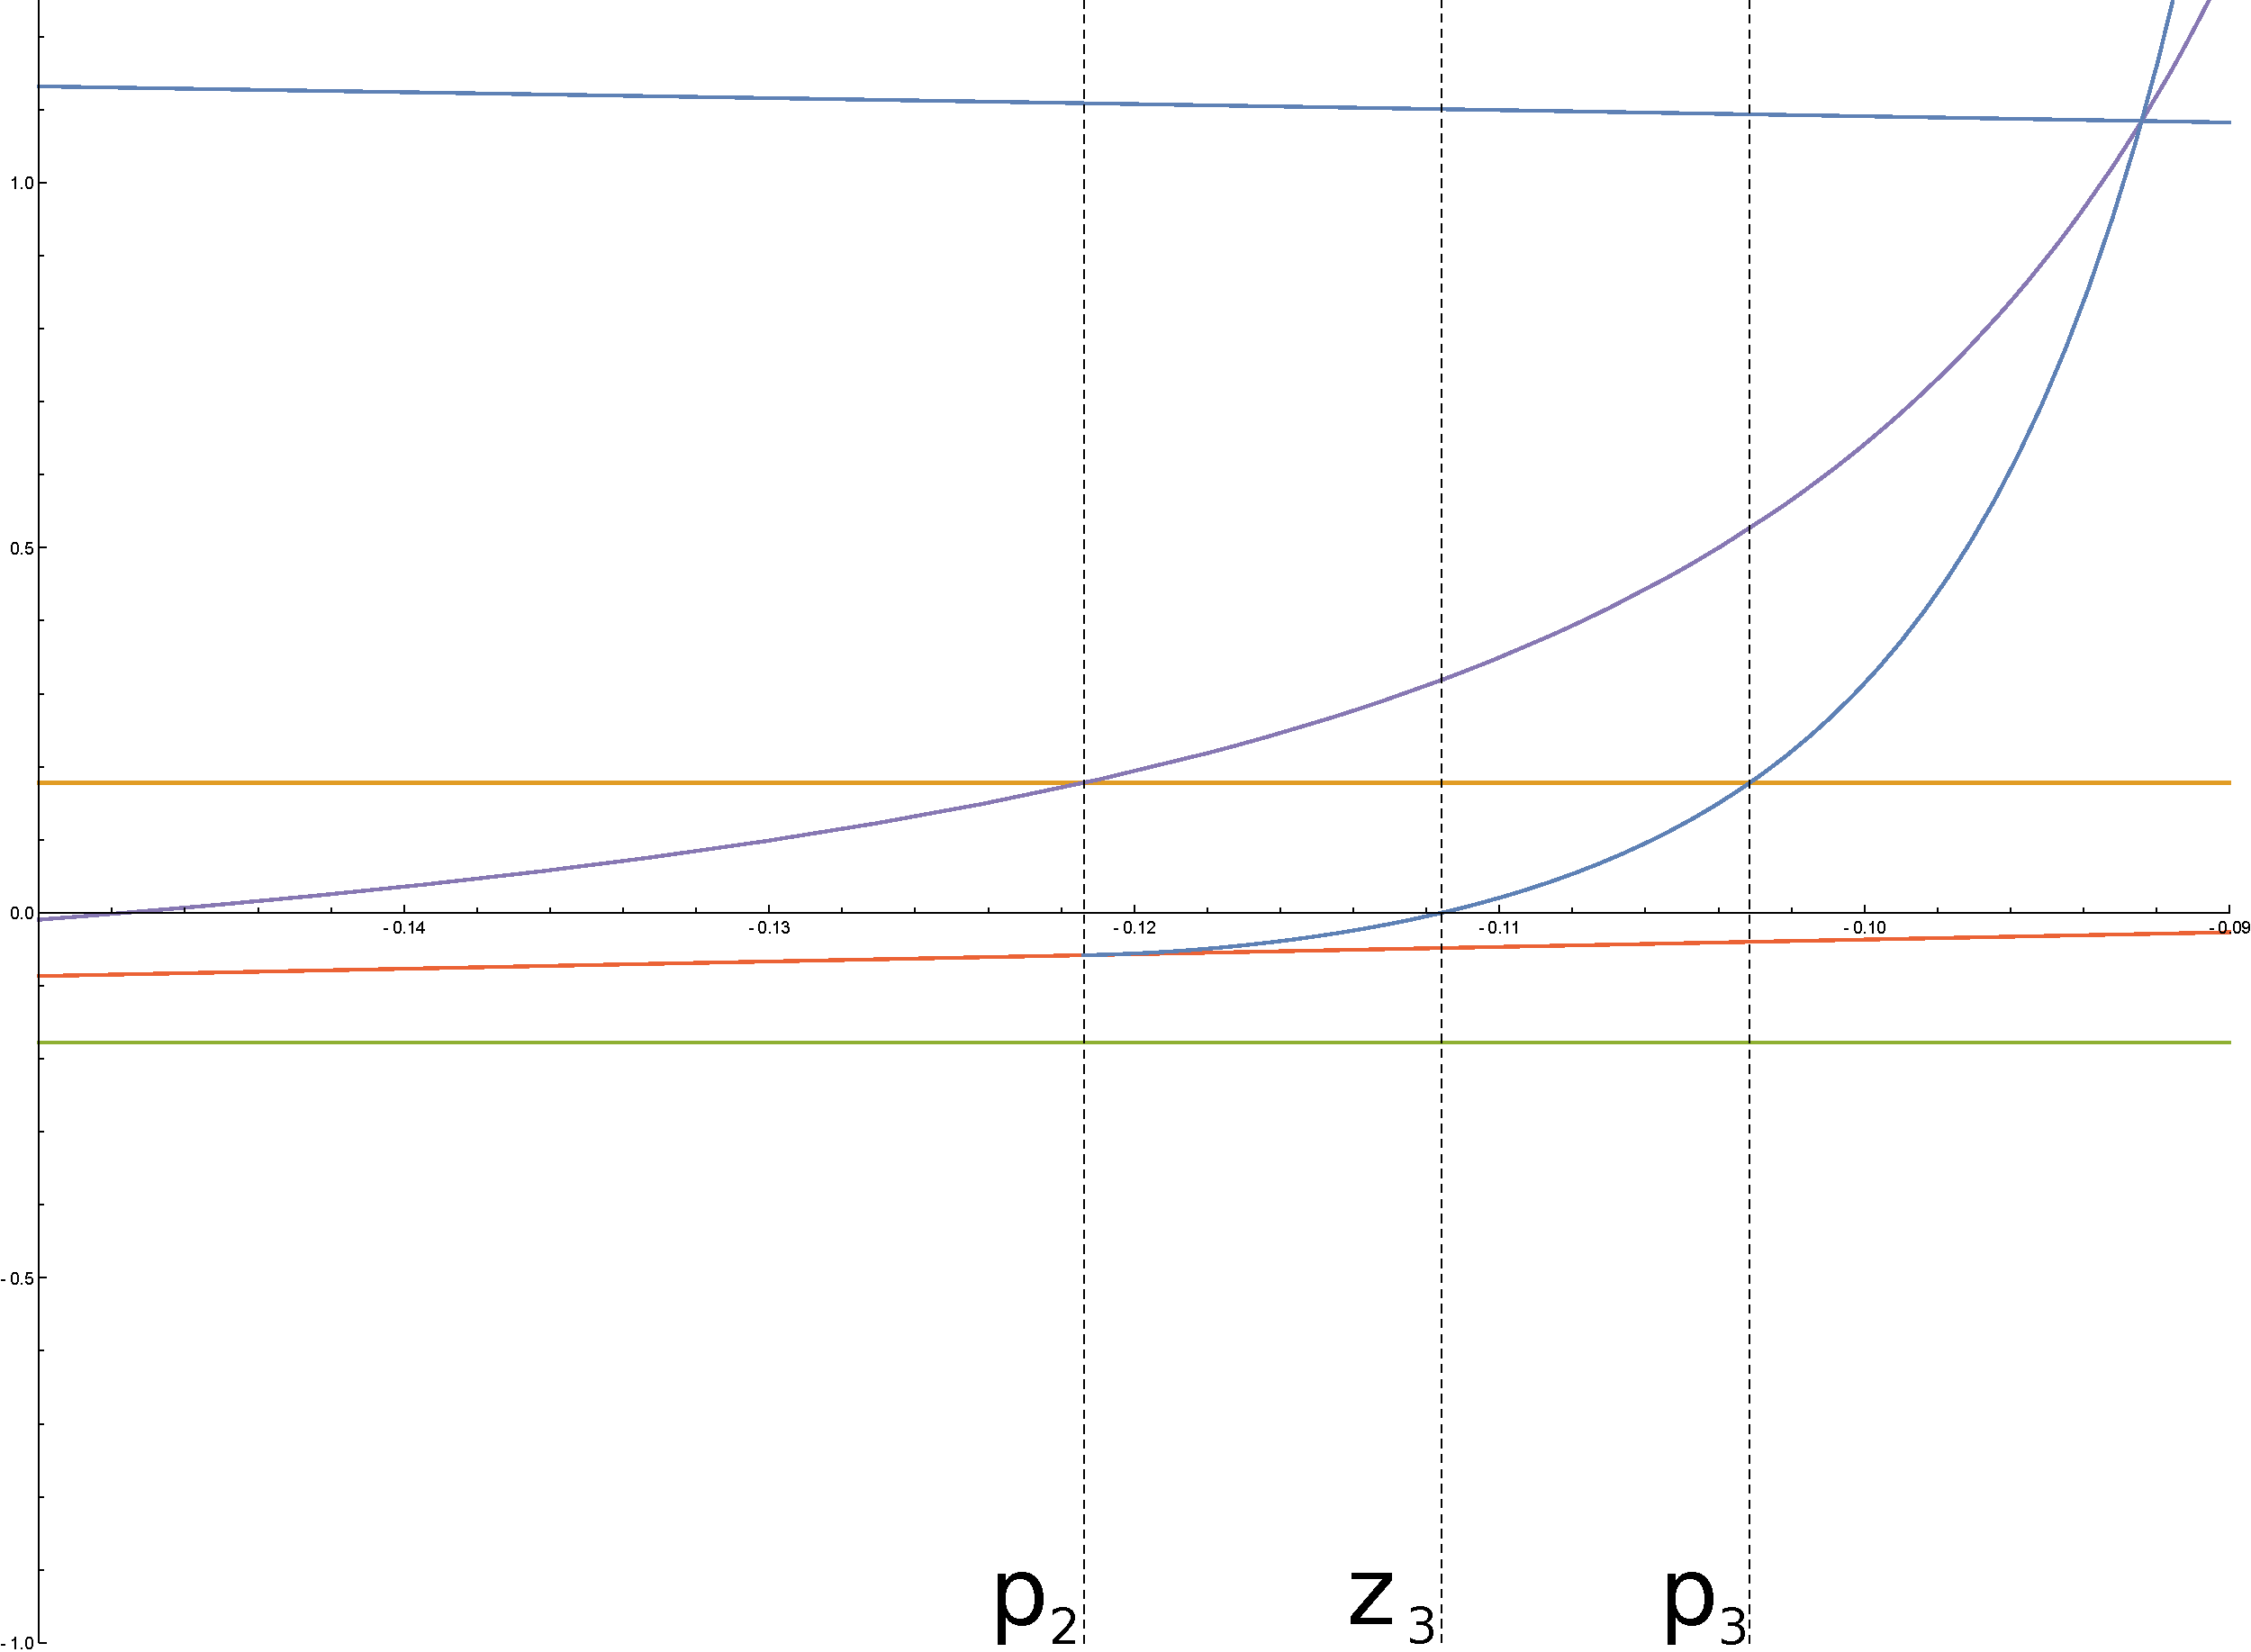
\includegraphics[width=\textwidth]{./img/cplot2H}
				\caption{$n=3$}
				\label{fig:cplot2H}
		\end{subfigure}
		\begin{subfigure}[b]{0.5\textwidth}
				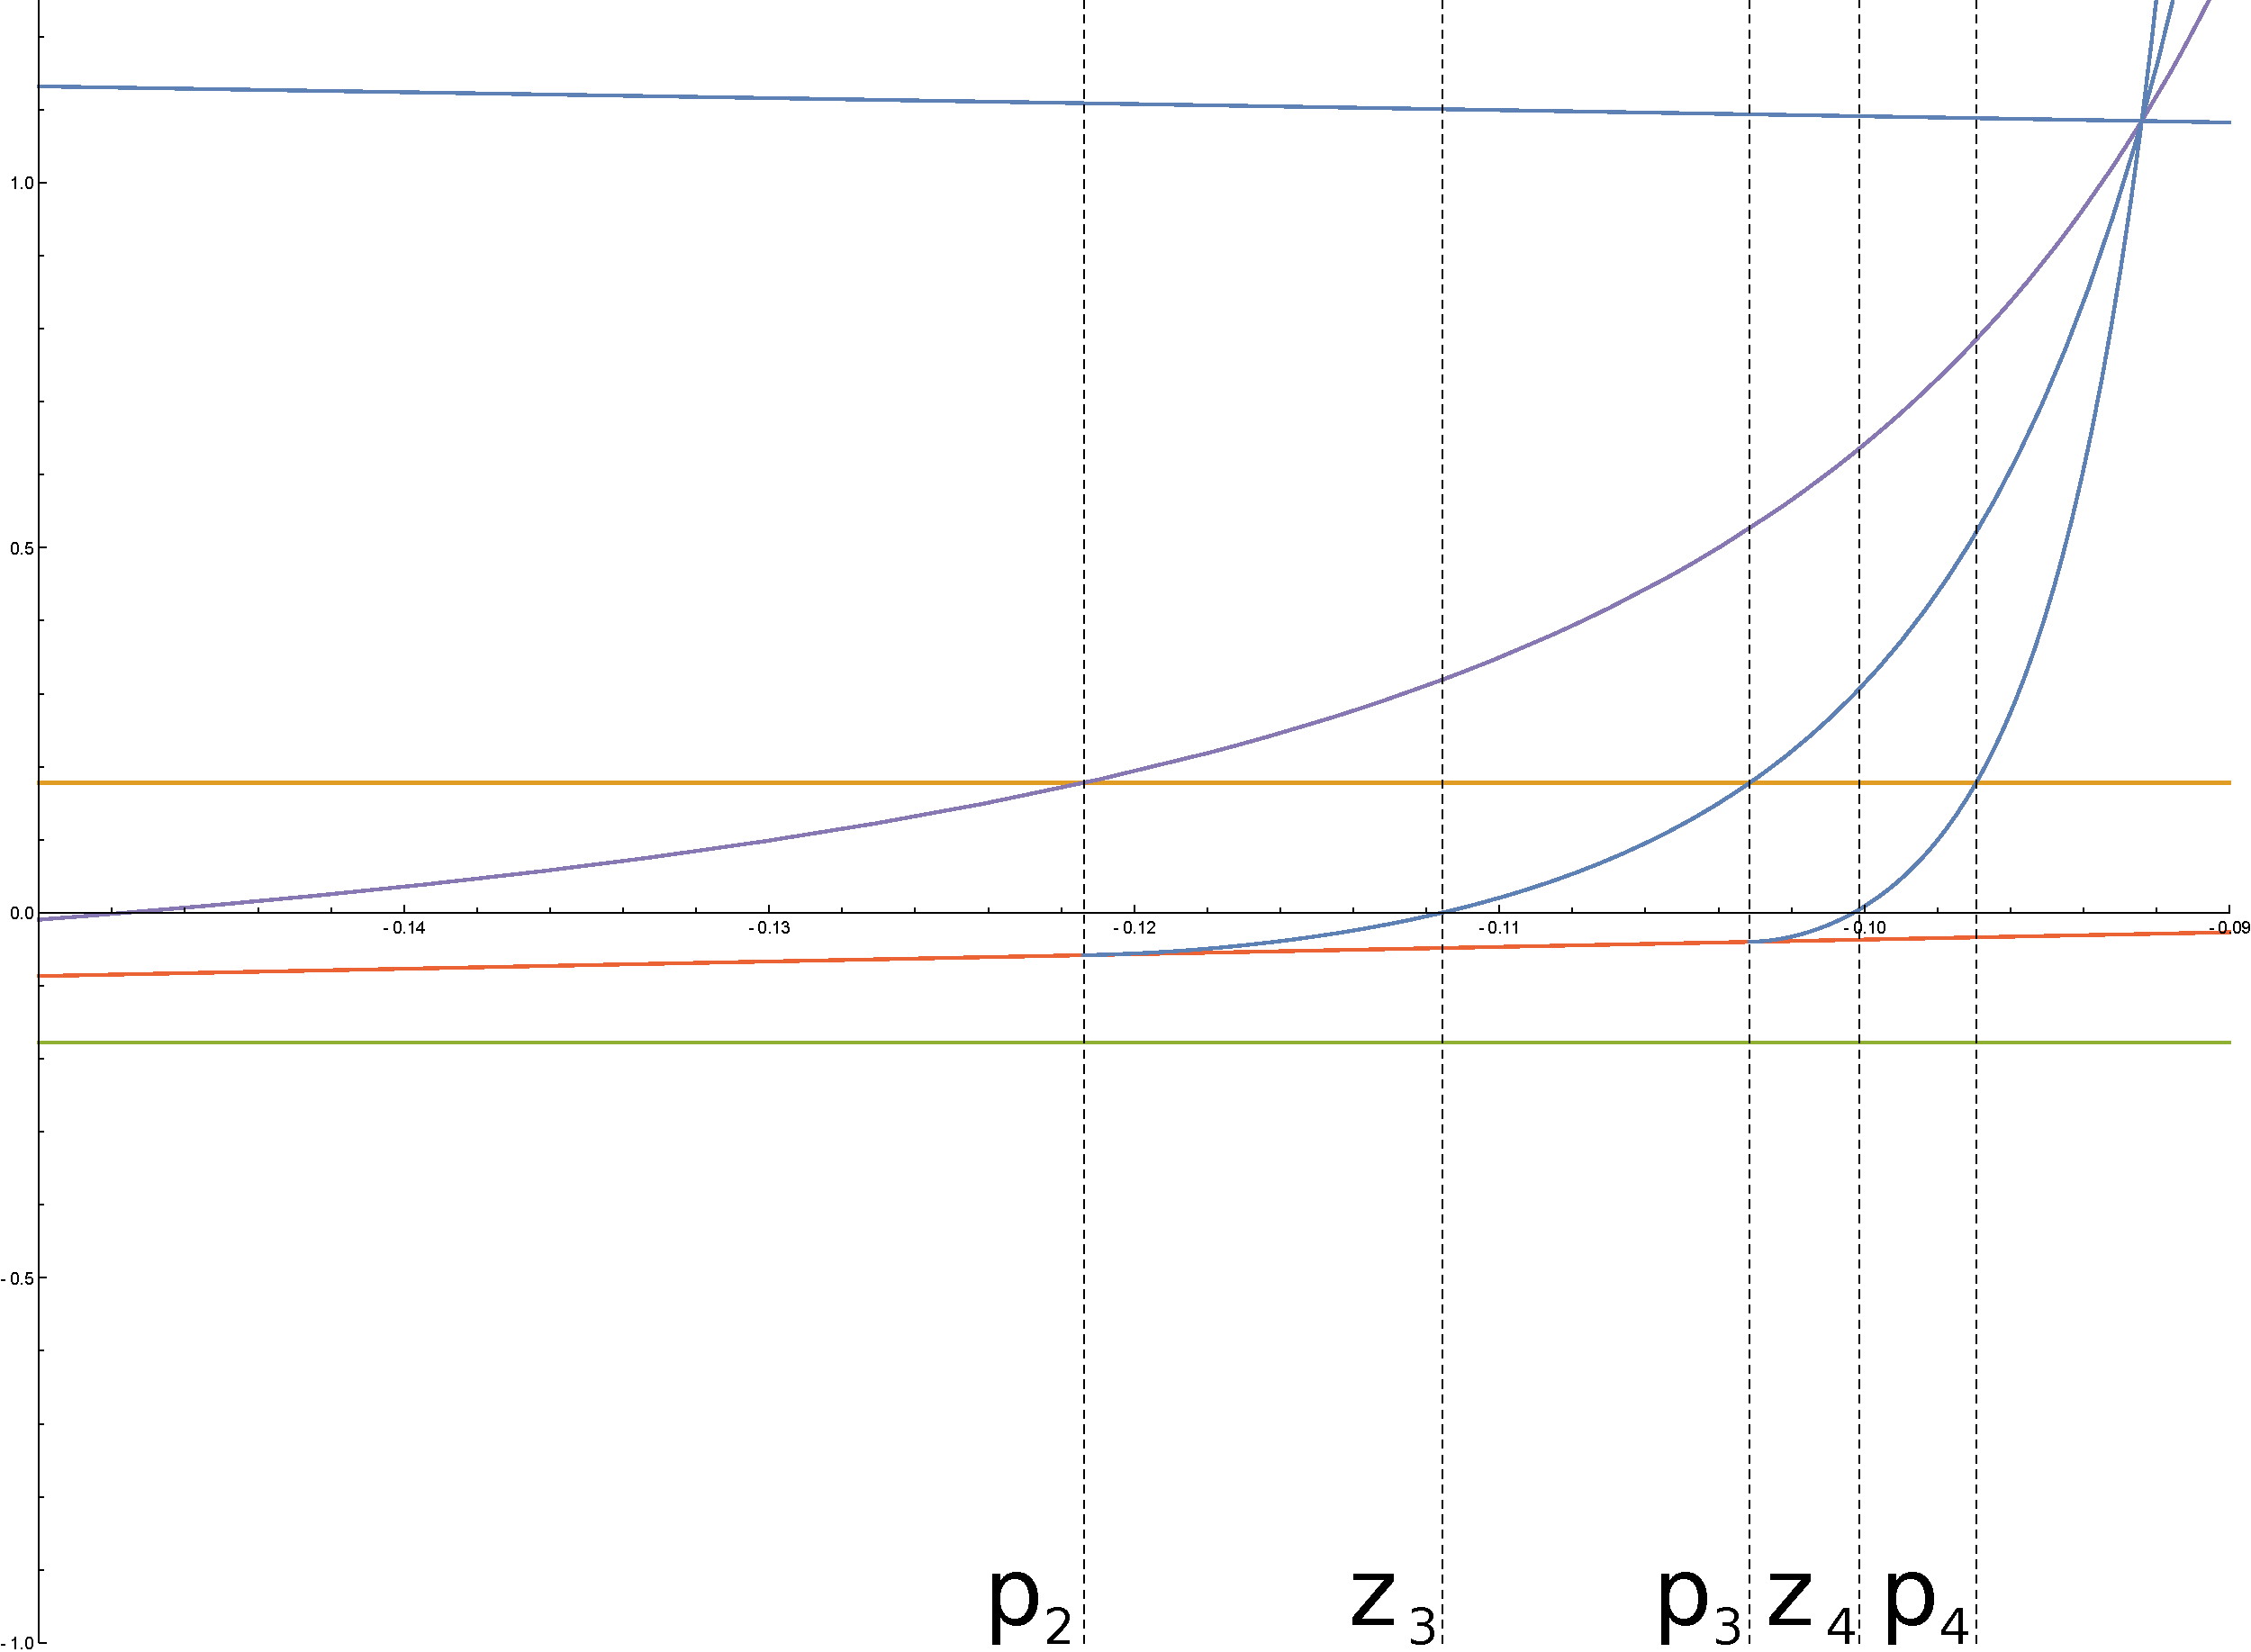
\includegraphics[width=\textwidth]{./img/cplot3H}
				\caption{$n=4$}
				\label{fig:cplot3H}
		\end{subfigure}%
		~ %add desired spacing between images, e. g. ~, \quad, \qquad, \hfill etc.
		  % (or a blank line to force the subfigure onto a new line)
		\begin{subfigure}[b]{0.5\textwidth}
				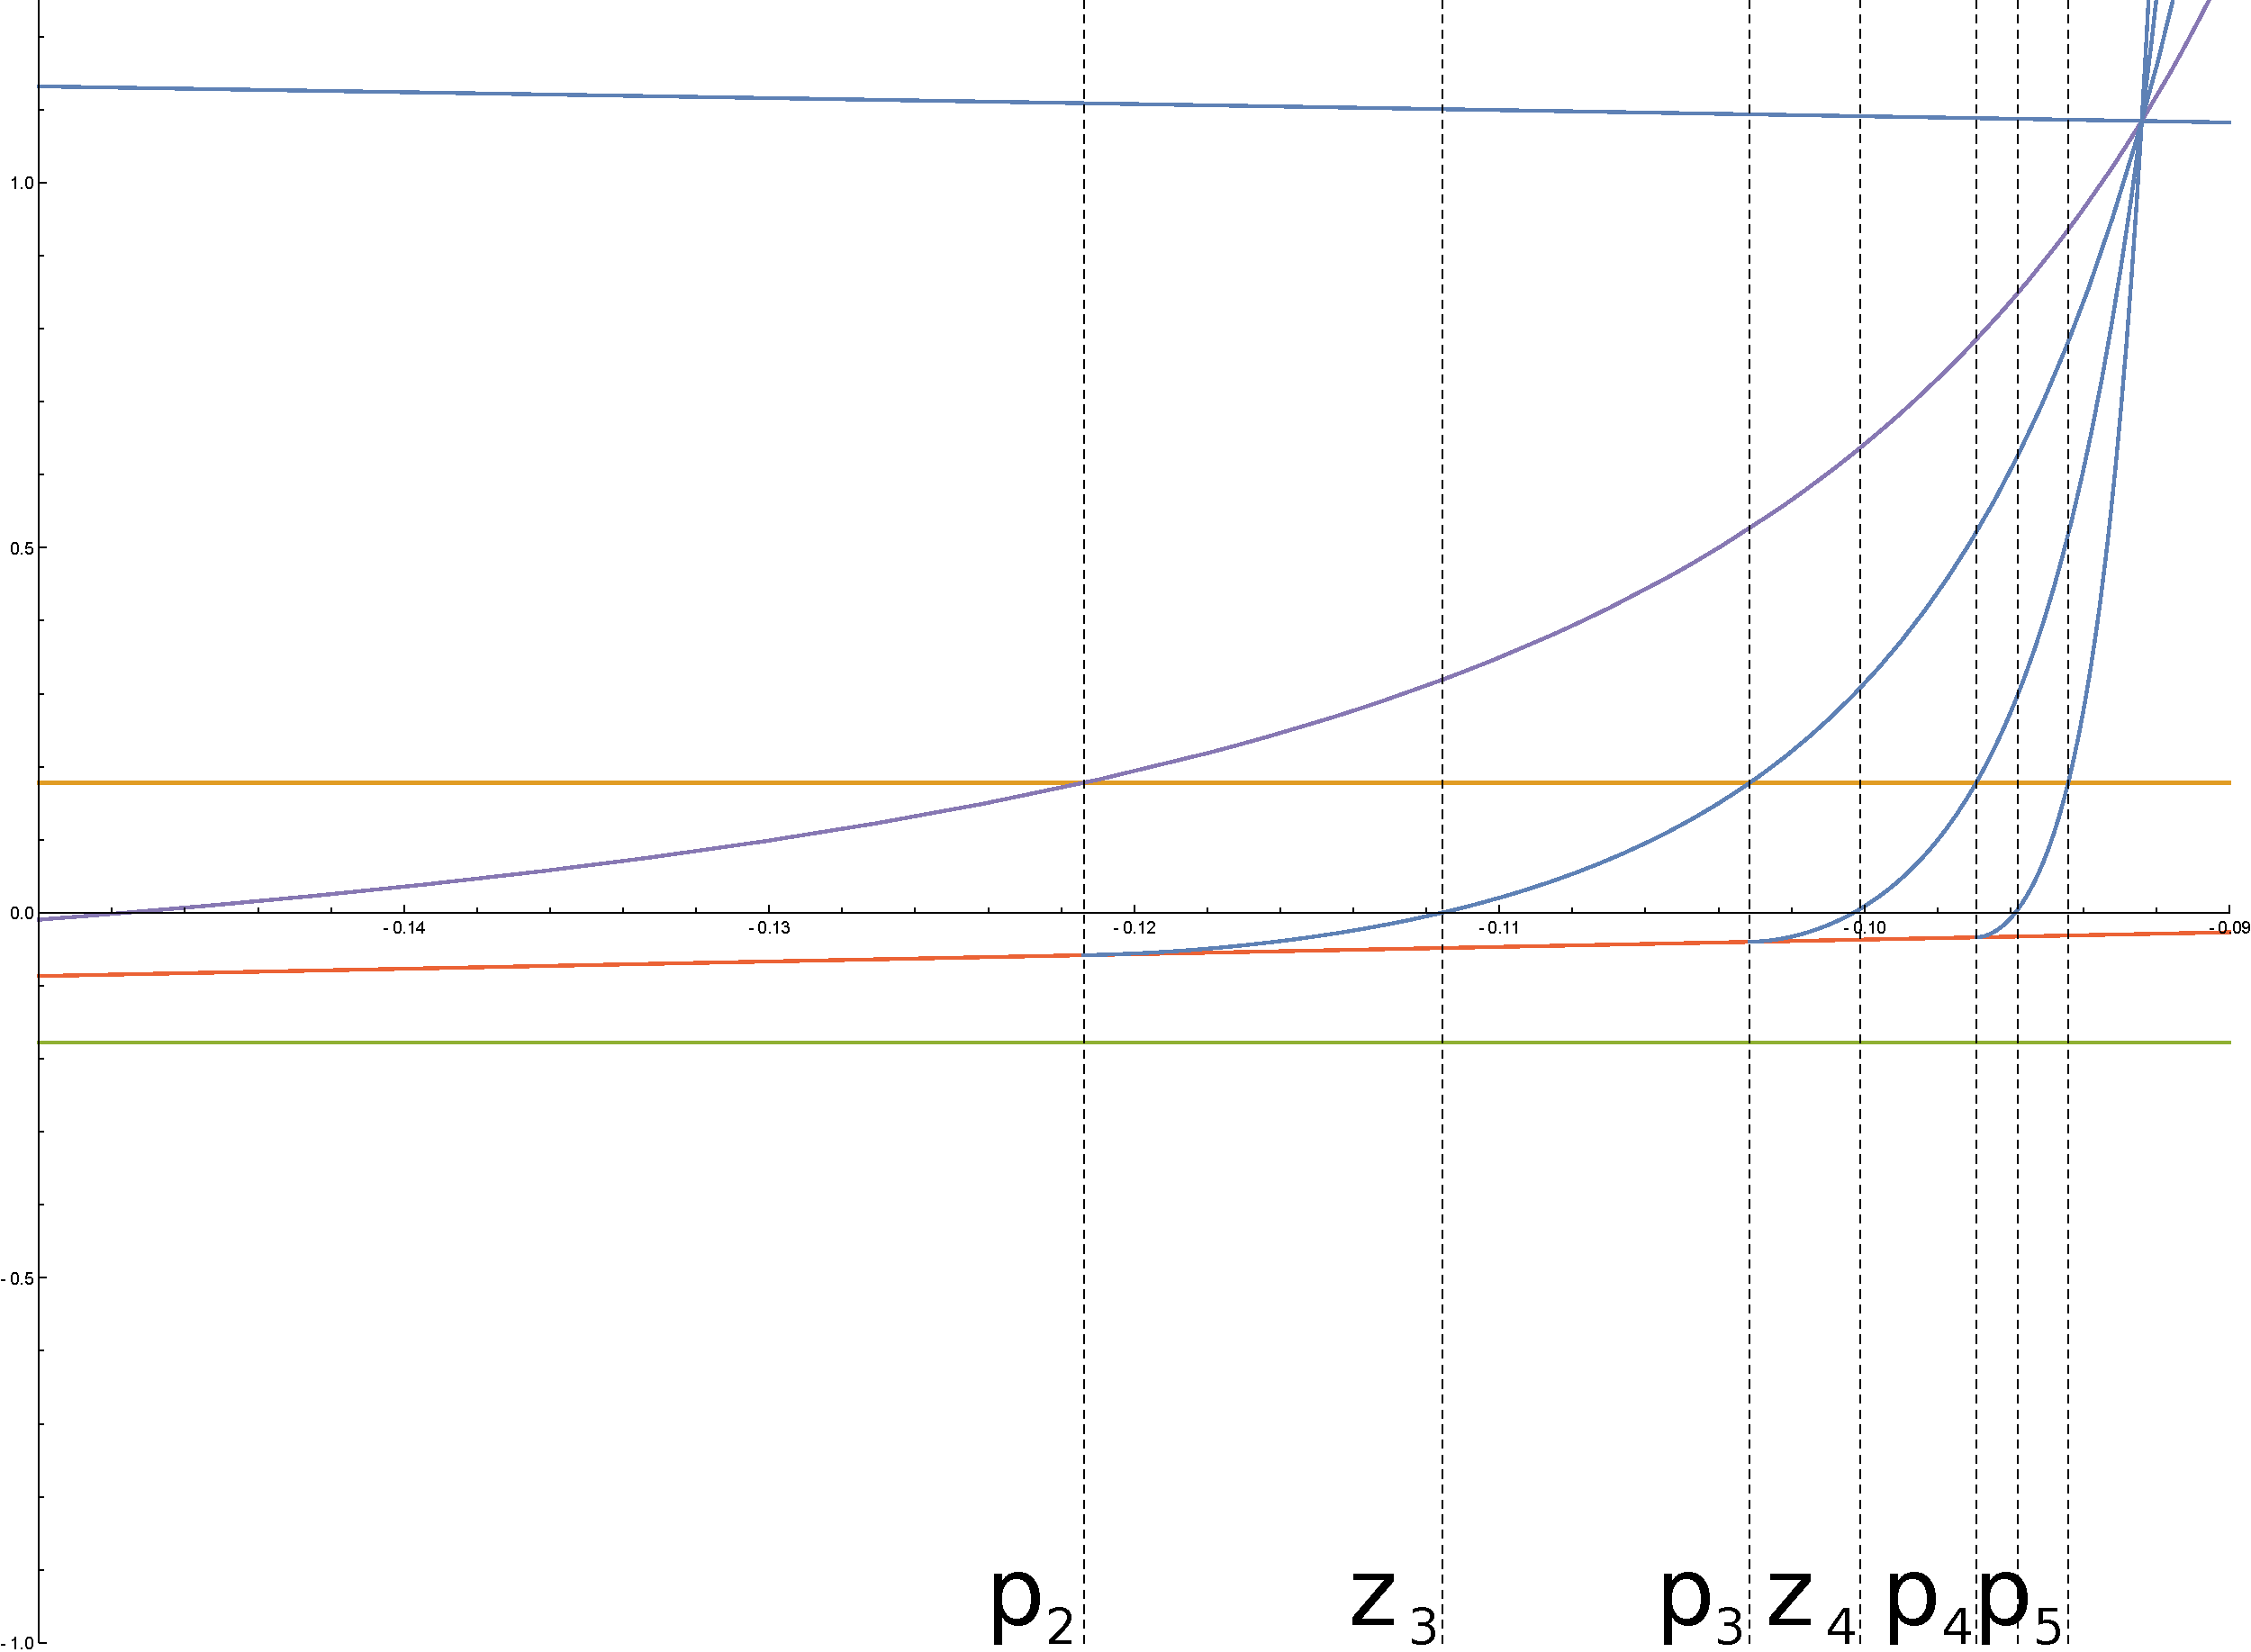
\includegraphics[width=\textwidth]{./img/cplot4H}
				\caption{$n=5$}
				\label{fig:cplot4H}
		\end{subfigure}
		\begin{subfigure}[b]{0.5\textwidth}
				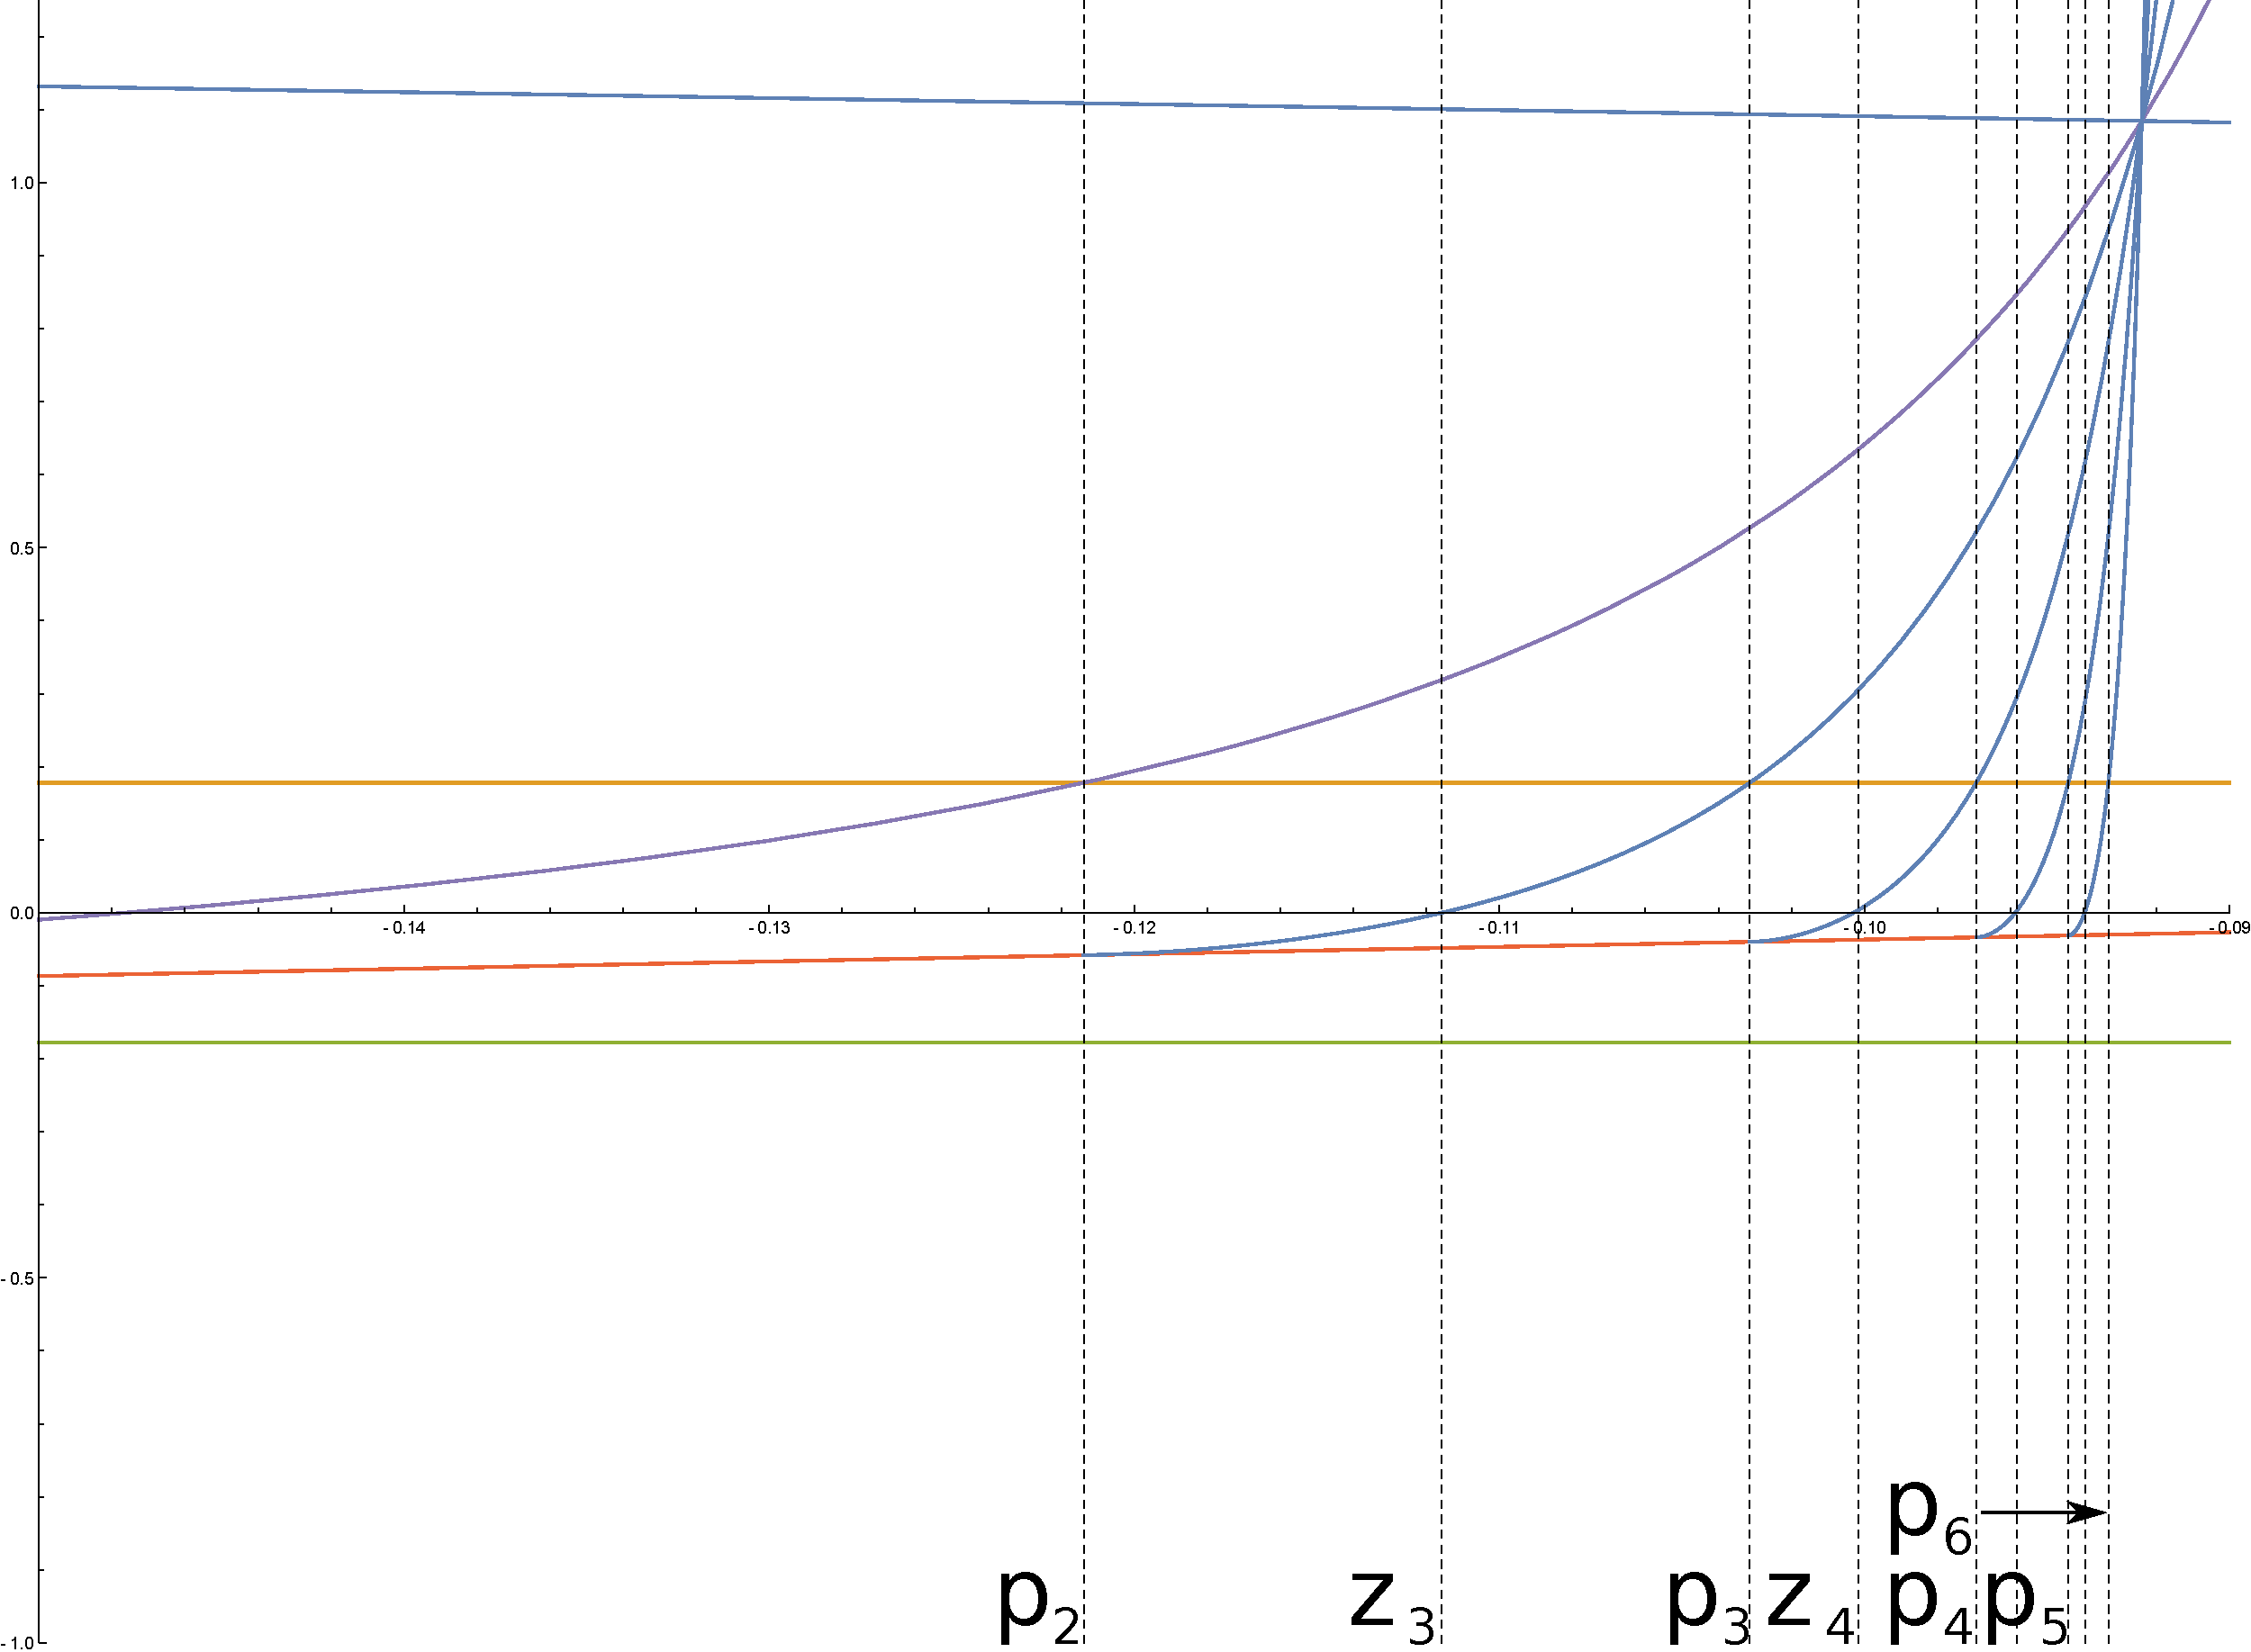
\includegraphics[width=\textwidth]{./img/cplot5H}
				\caption{$n=6$}
				\label{fig:cplot5H}
		\end{subfigure}%
		~ %add desired spacing between images, e. g. ~, \quad, \qquad, \hfill etc.
		  % (or a blank line to force the subfigure onto a new line)
		\begin{subfigure}[b]{0.5\textwidth}
				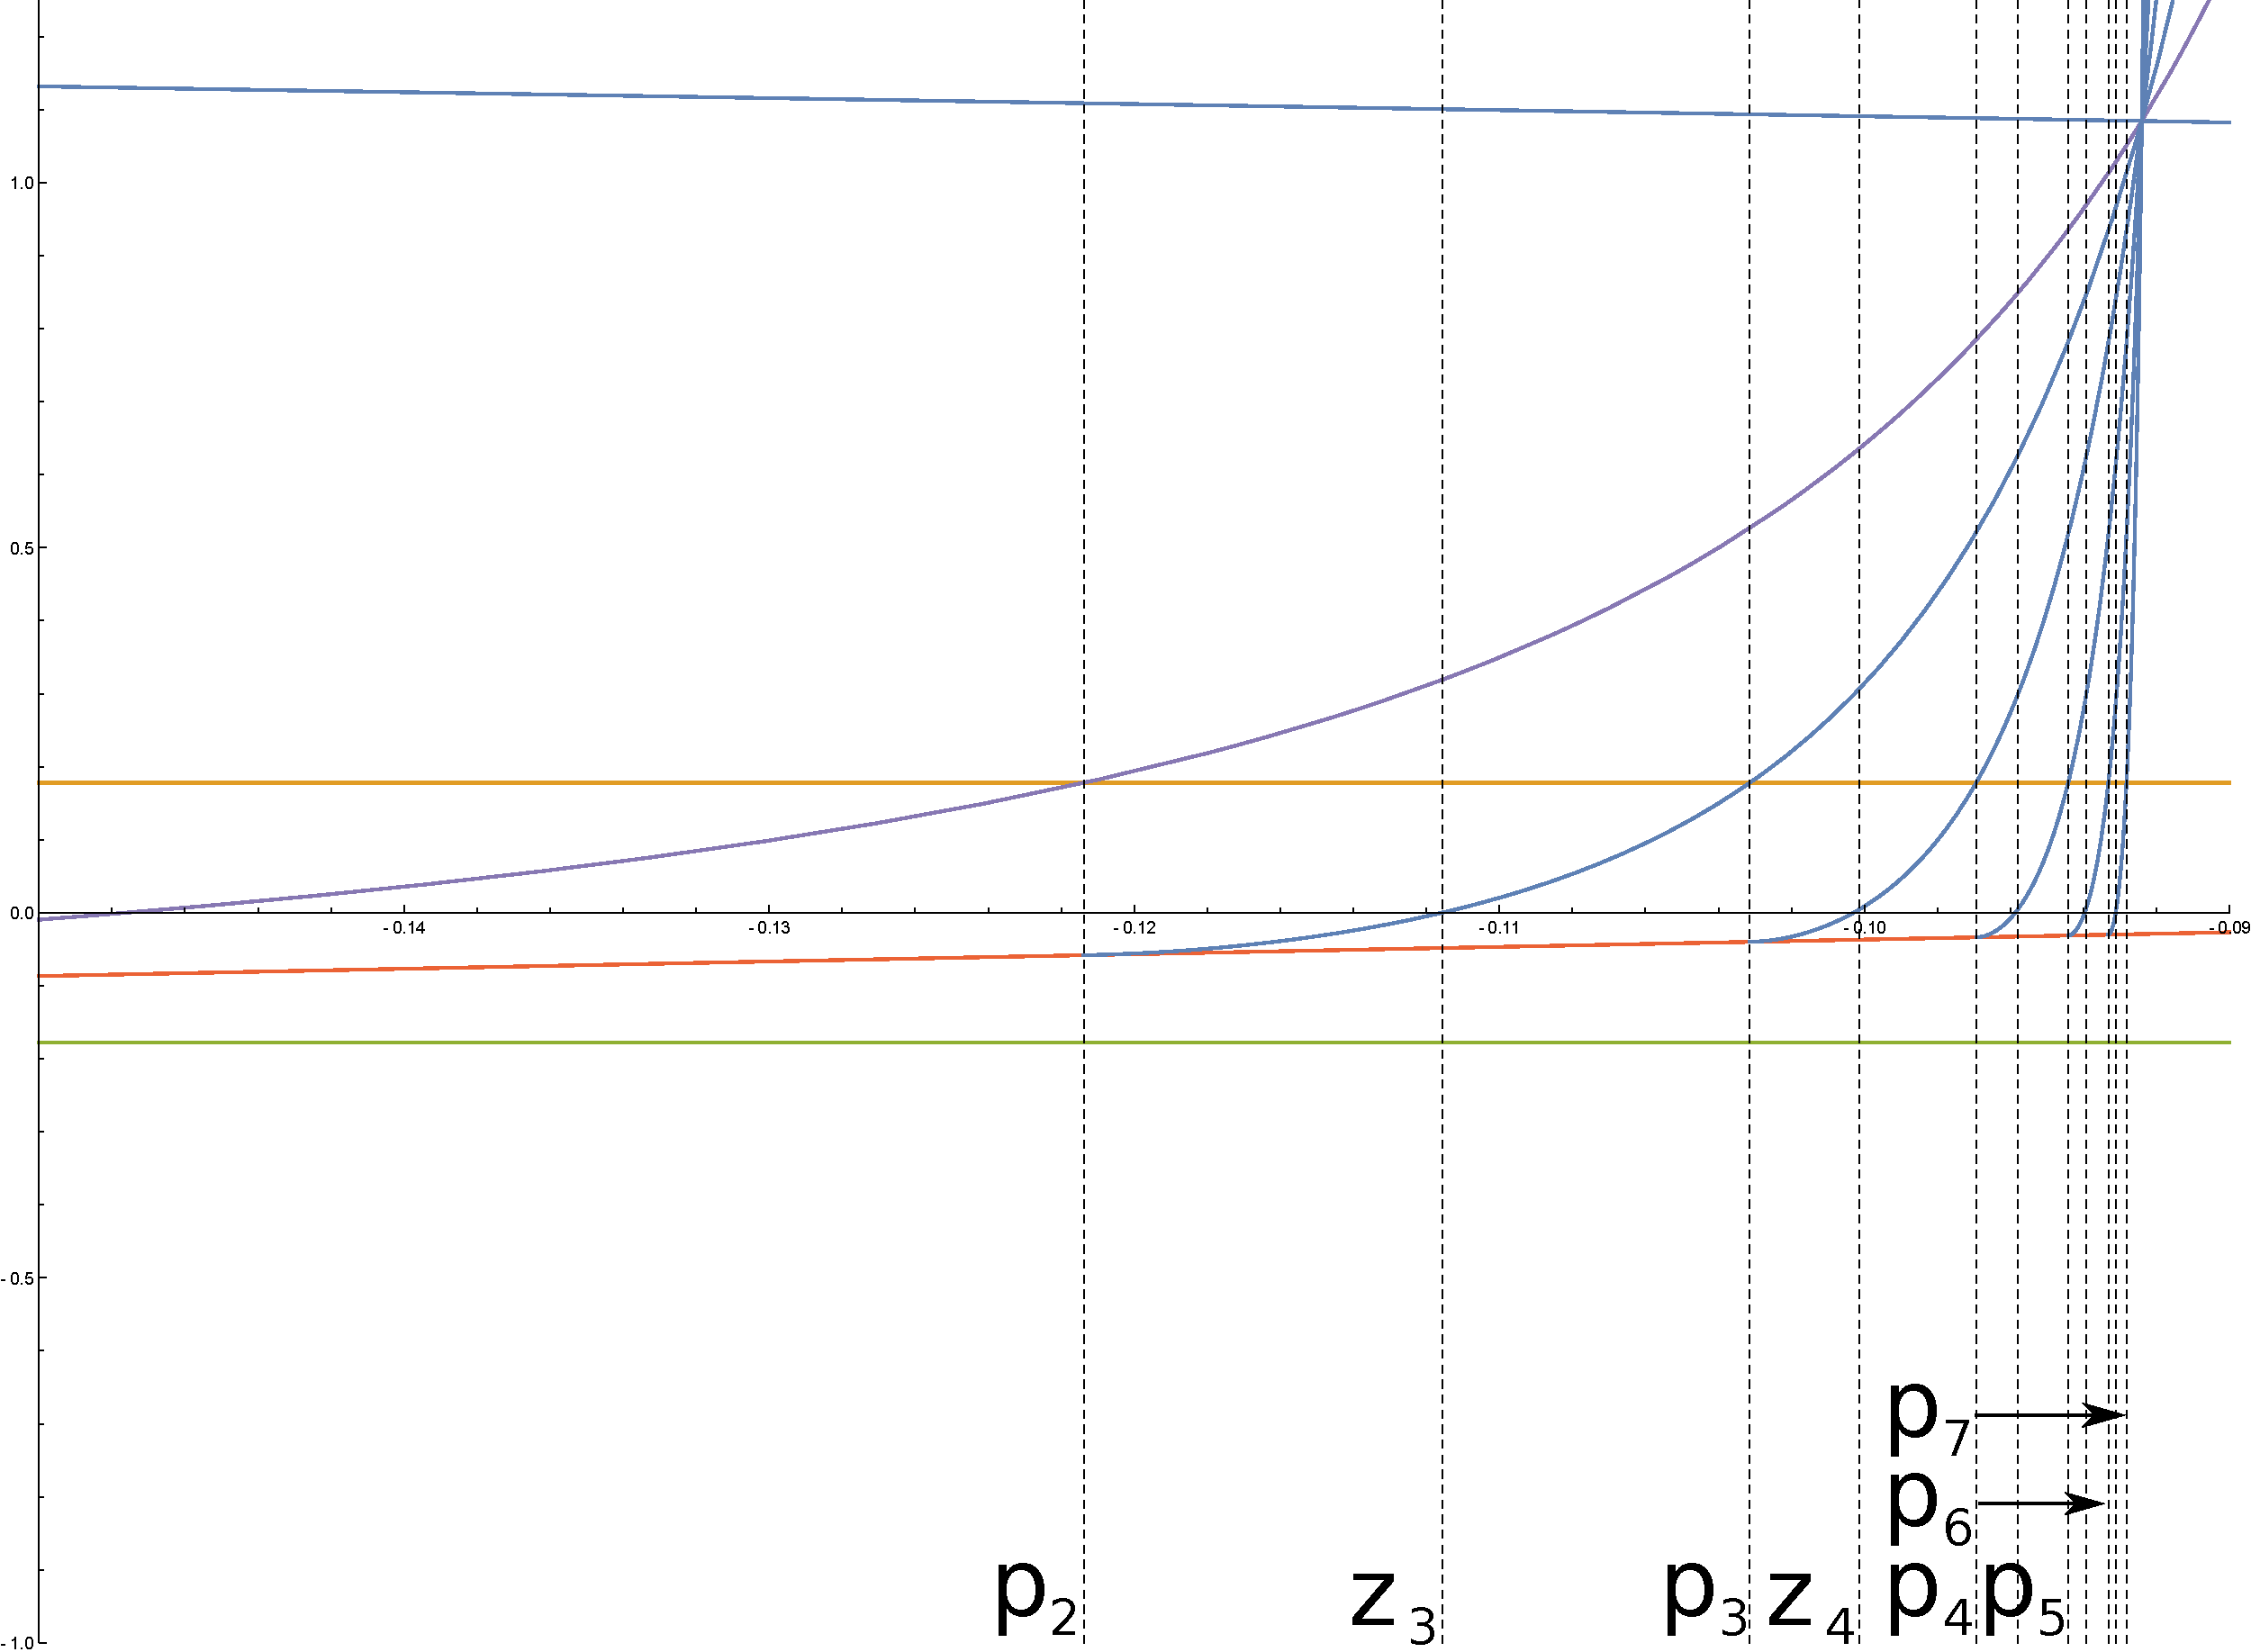
\includegraphics[width=\textwidth]{./img/cplot6H}
				\caption{$n=7$}
				\label{fig:cplot6H}
		\end{subfigure}
		~ %add desired spacing between images, e. g. ~, \quad, \qquad, \hfill etc.
		  % (or a blank line to force the subfigure onto a new line)
		\caption{Plots of various iterates of $f_c (C)$ as a function of $c$ depicting the accumulation of prezero and periodic parameter values as we approach $h_2^{CrP_c}$ from the left. Note that for $n > 4$ the $z_n$ values are marked but not labeled. Also observe that each $f^i_c (C)$ is only plotted on the interval $ (p_{i-1}, h_2^{CrP_c})$ in order to highlight specific behaviors}\label{fig:iterh1}
\end{figure}

% \begin{figure}[ht]
% 		\centering
% 		\begin{subfigure}[b]{0.5\textwidth}
% 				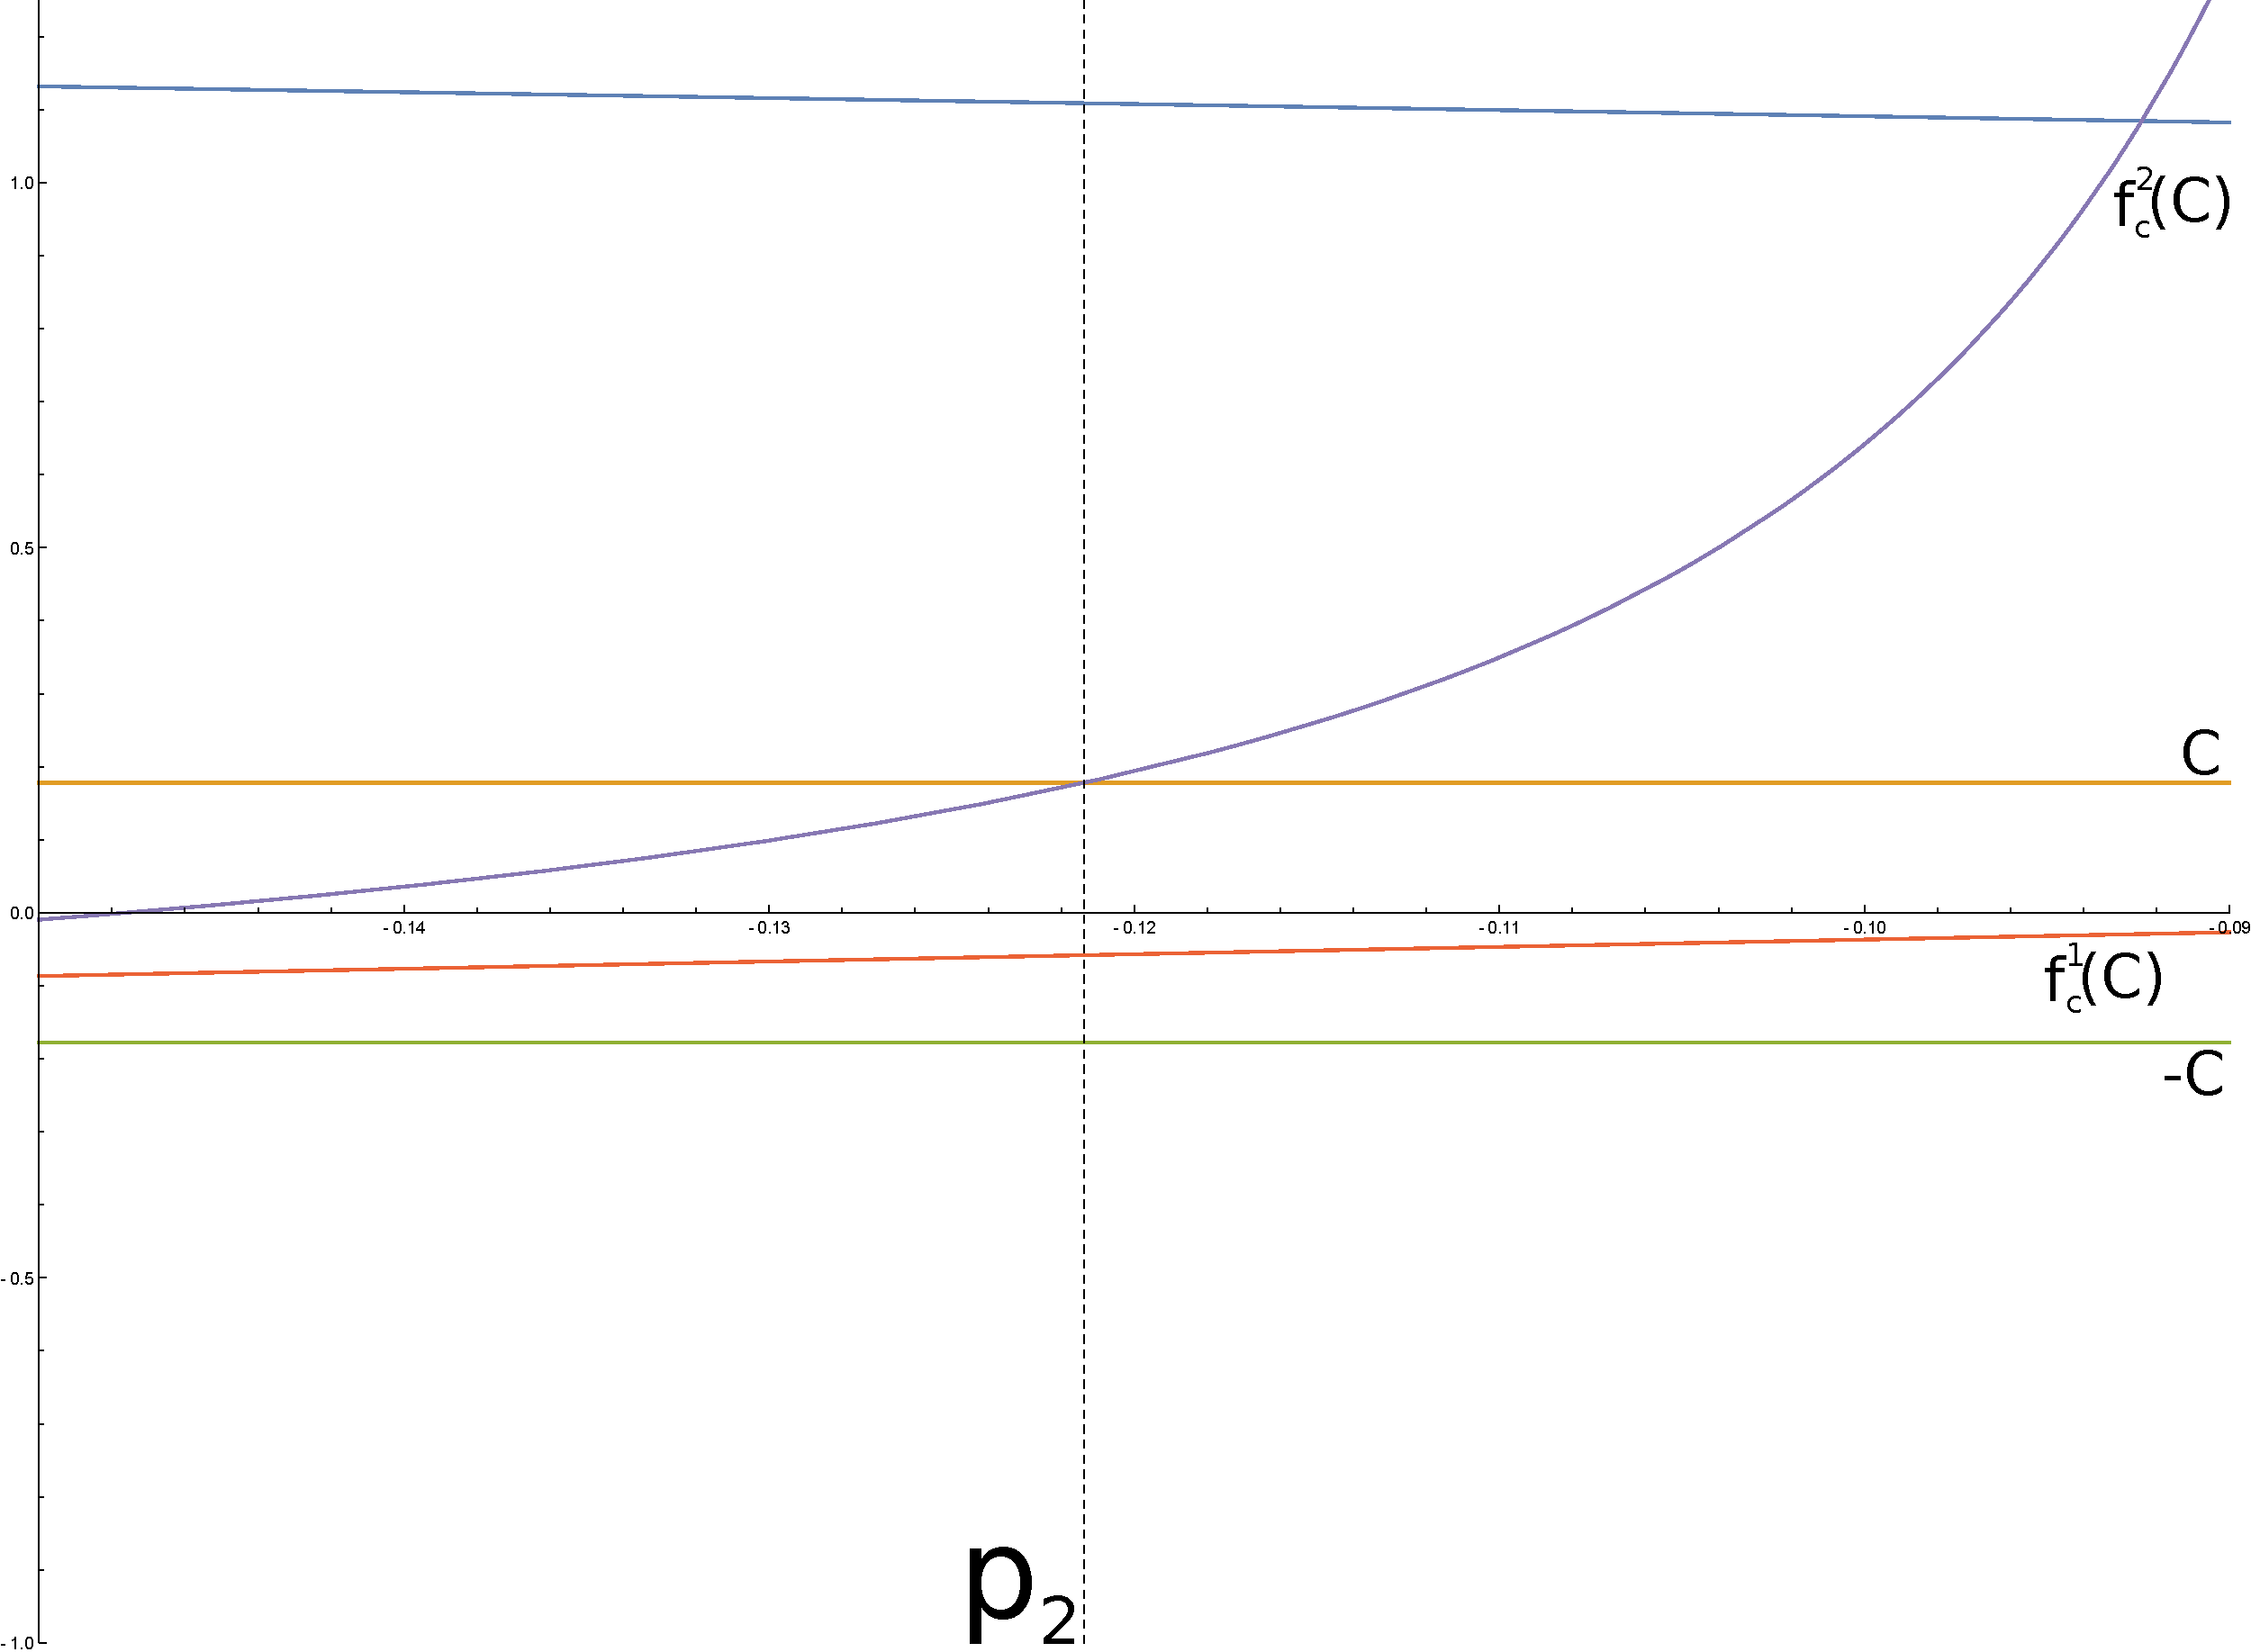
\includegraphics[width=\textwidth]{./img/cplot1H}
% 				\caption{First two iterates of $f_c (C)$ along with the parameter value of its superattracting periodic orbit}
% 				\label{fig:cplot1H}
% 		\end{subfigure}%
% 		~ %add desired spacing between images, e. g. ~, \quad, \qquad, \hfill etc.
% 		  % (or a blank line to force the subfigure onto a new line)
% 		\begin{subfigure}[b]{0.5\textwidth}
% 				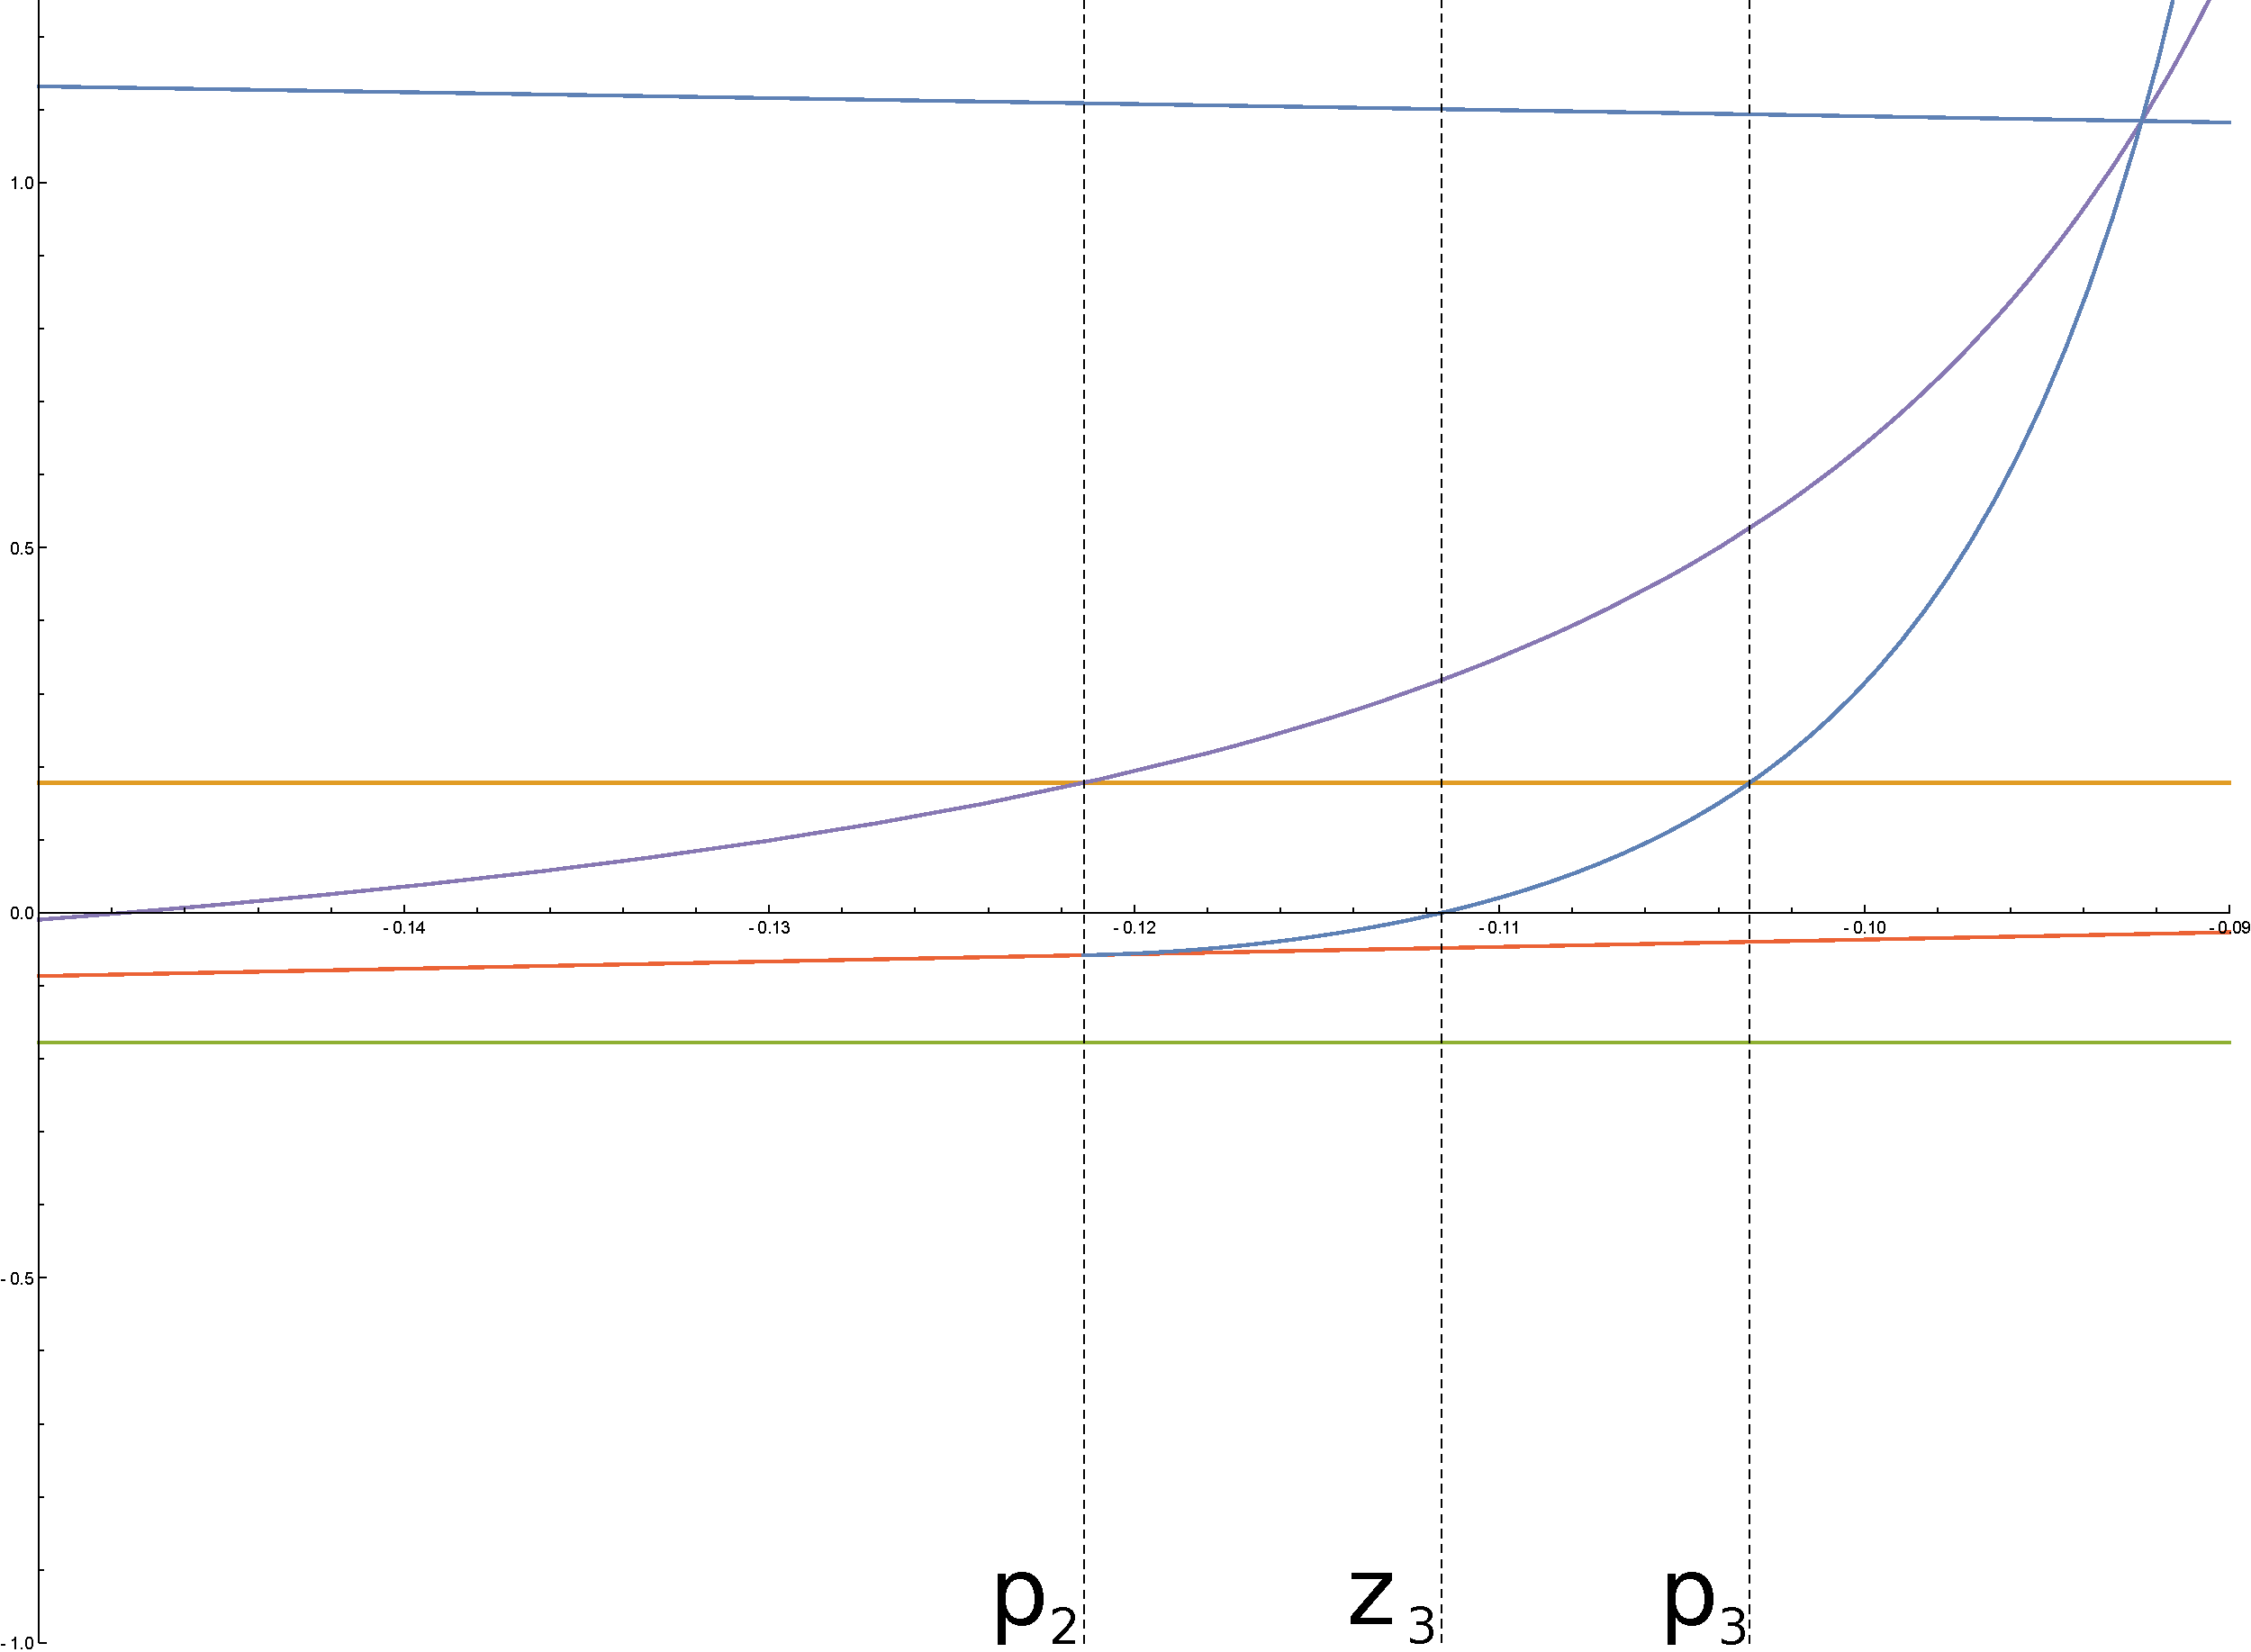
\includegraphics[width=\textwidth]{./img/cplot2H}
% 				\caption{Third iterate of $f_c (C)$ added along with the parameter value of its superattracting periodic orbit}
% 				\label{fig:cplot2H}
% 		\end{subfigure}
% 		\begin{subfigure}[b]{0.5\textwidth}
% 				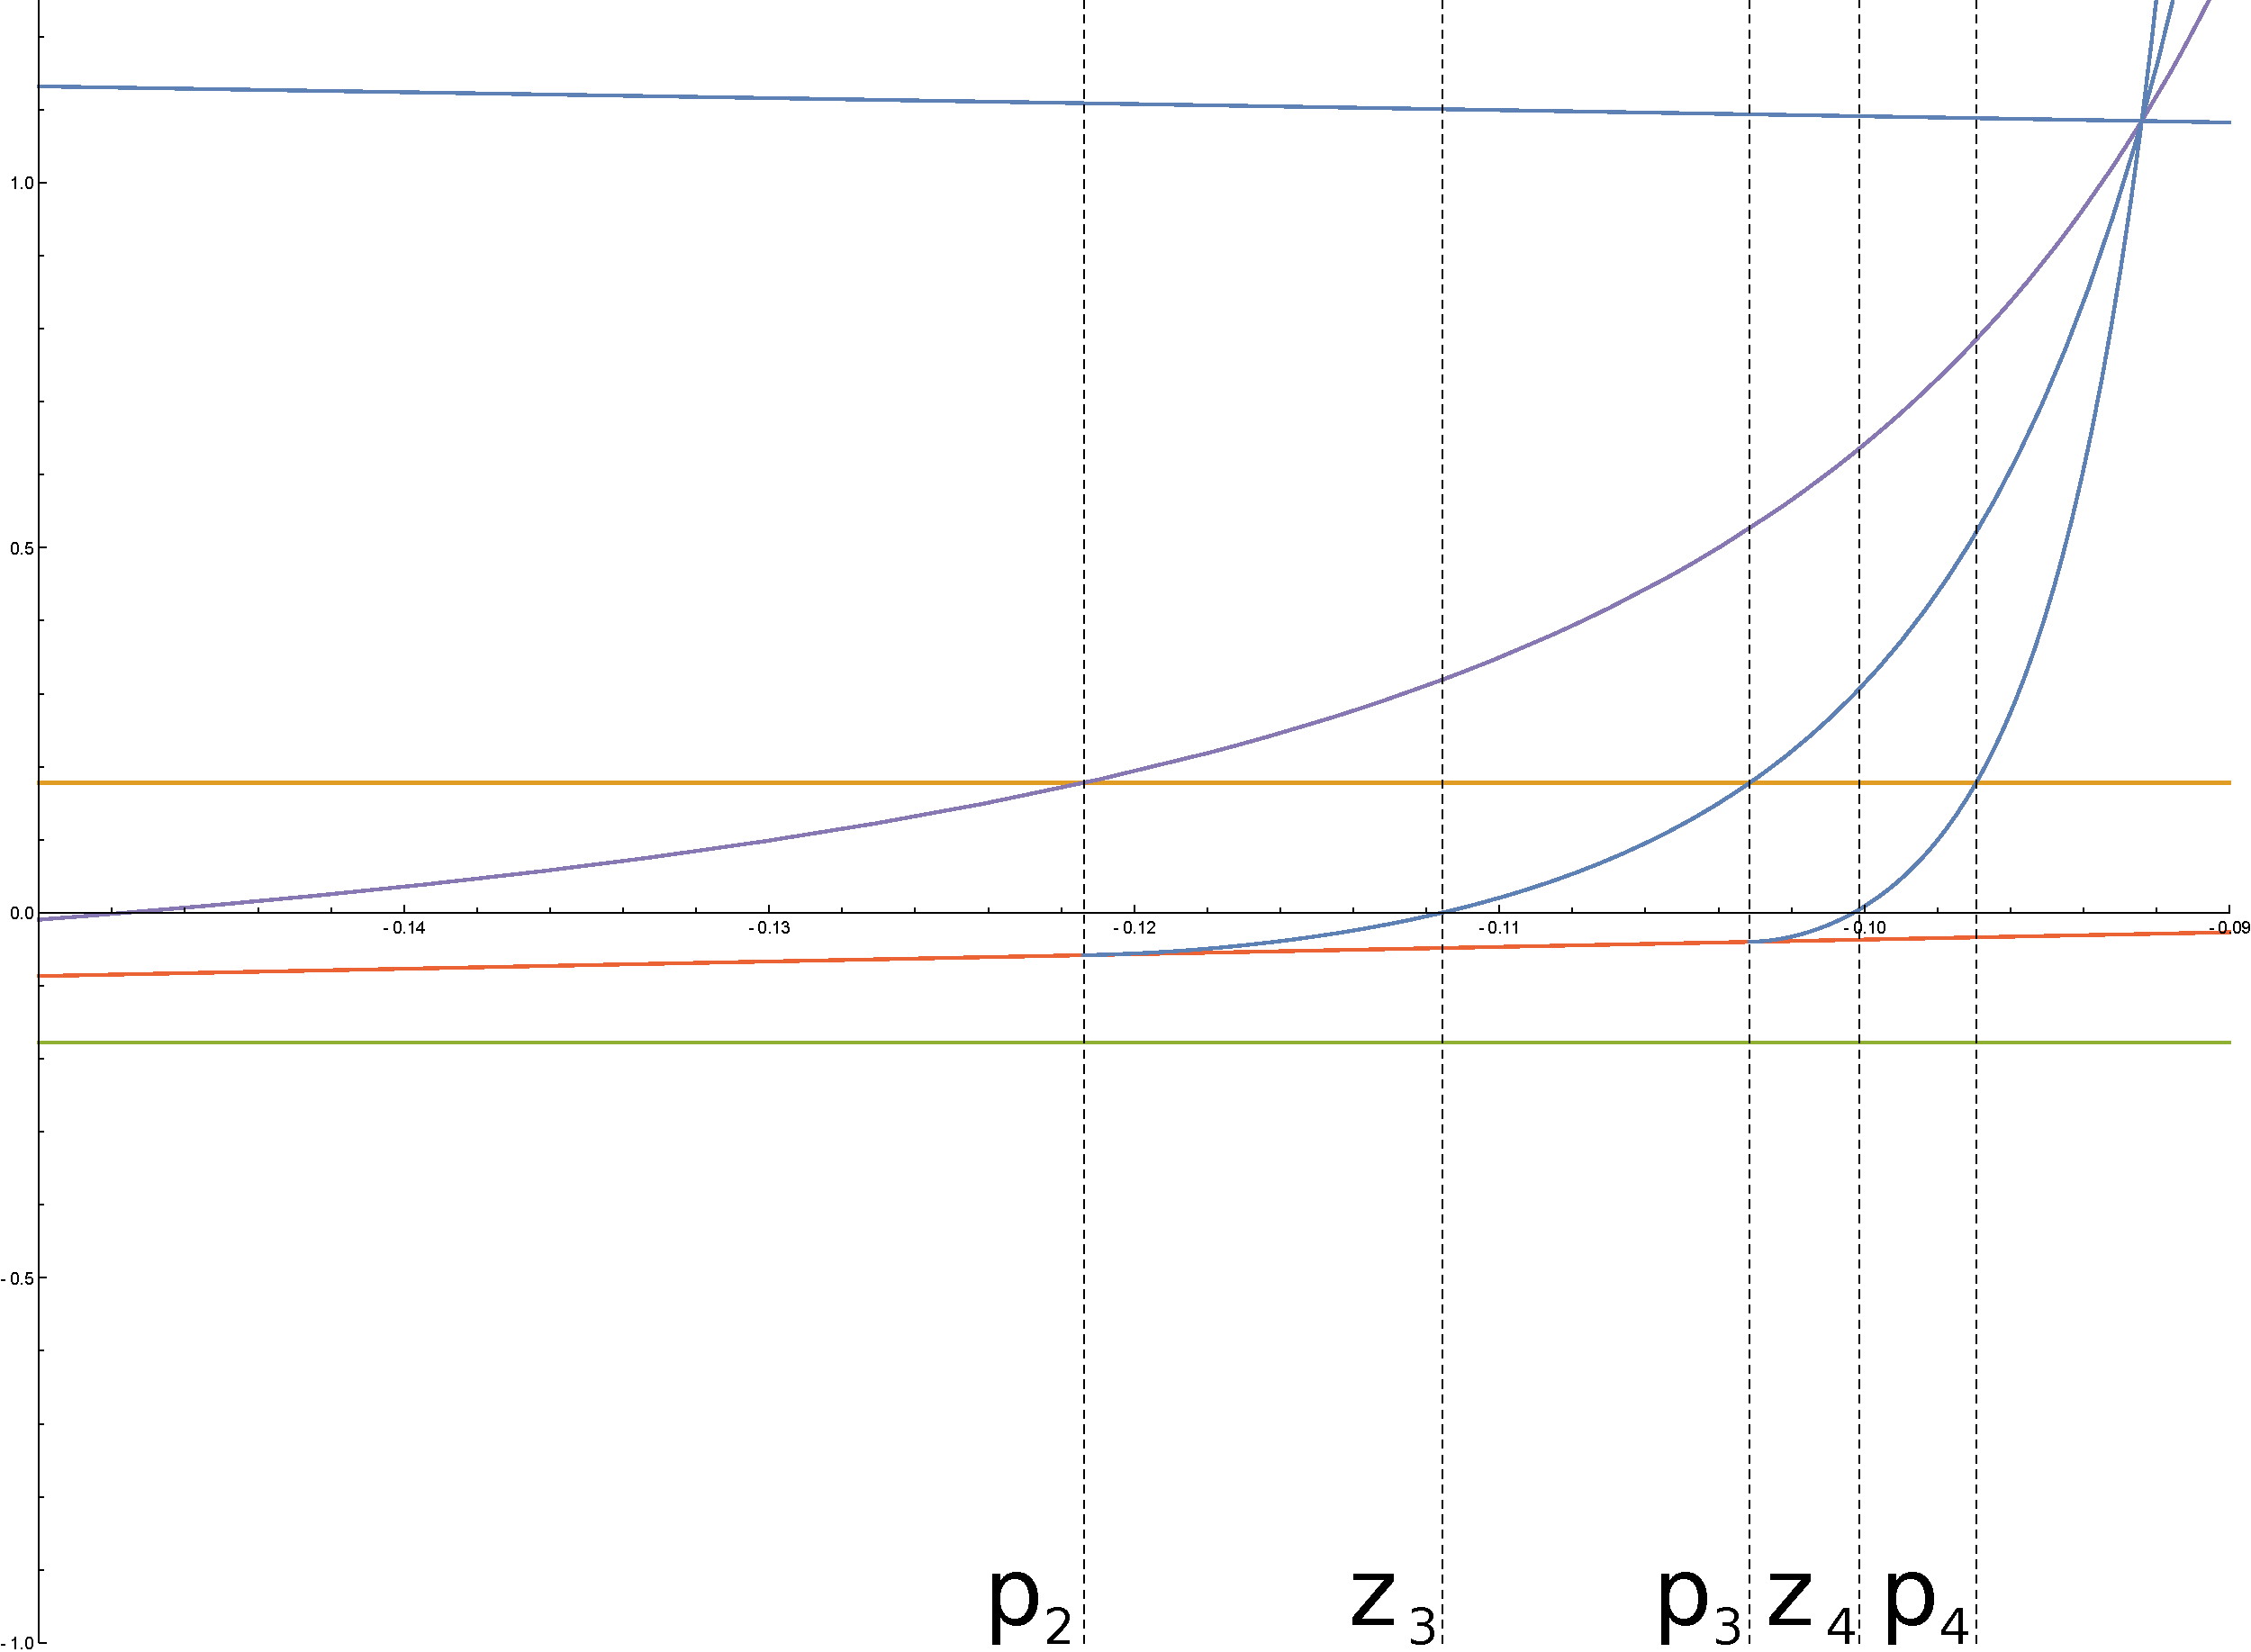
\includegraphics[width=\textwidth]{./img/cplot3H}
% 				\caption{Fourth iterate of $f_c (C)$ added along with the parameter value of its superattracting periodic orbit}
% 				\label{fig:cplot3H}
% 		\end{subfigure}%
% 		~ %add desired spacing between images, e. g. ~, \quad, \qquad, \hfill etc.
% 		  % (or a blank line to force the subfigure onto a new line)
% 		\begin{subfigure}[b]{0.5\textwidth}
% 				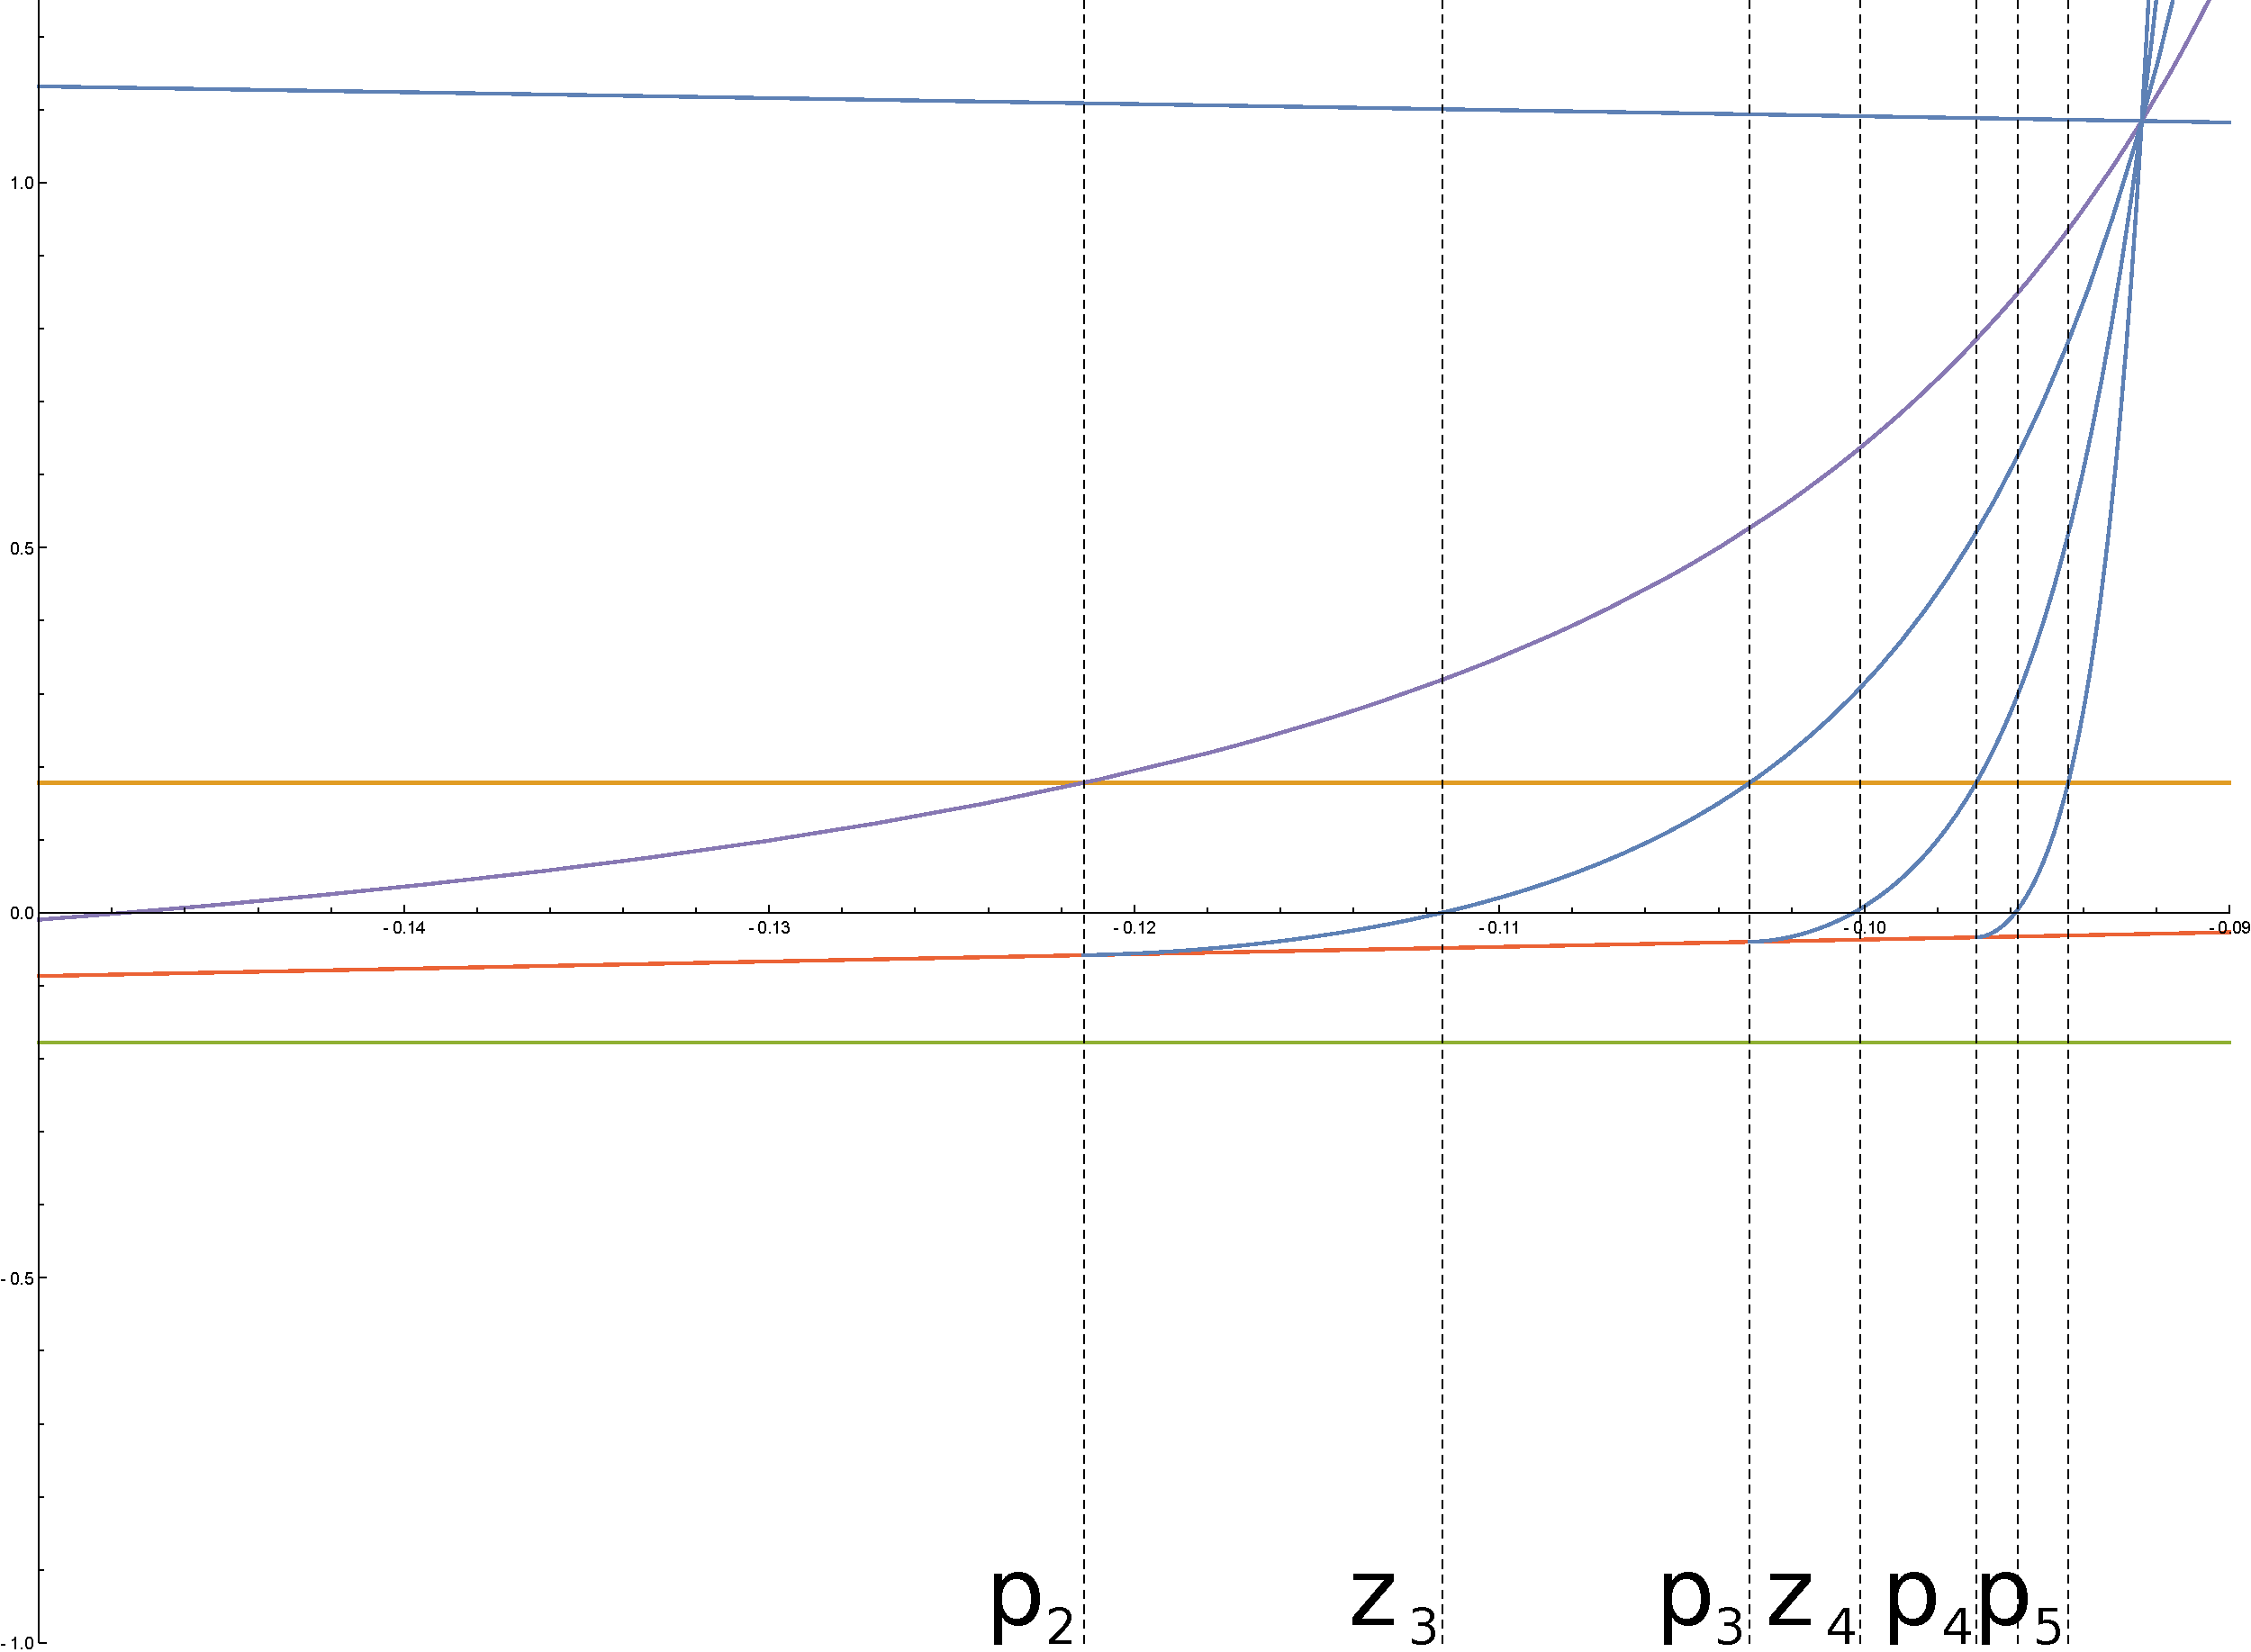
\includegraphics[width=\textwidth]{./img/cplot4H}
% 				\caption{Fifth iterate of $f_c (C)$ added along with the parameter value of its superattracting periodic orbit}
% 				\label{fig:cplot4H}
% 		\end{subfigure}
% 		\begin{subfigure}[b]{0.5\textwidth}
% 				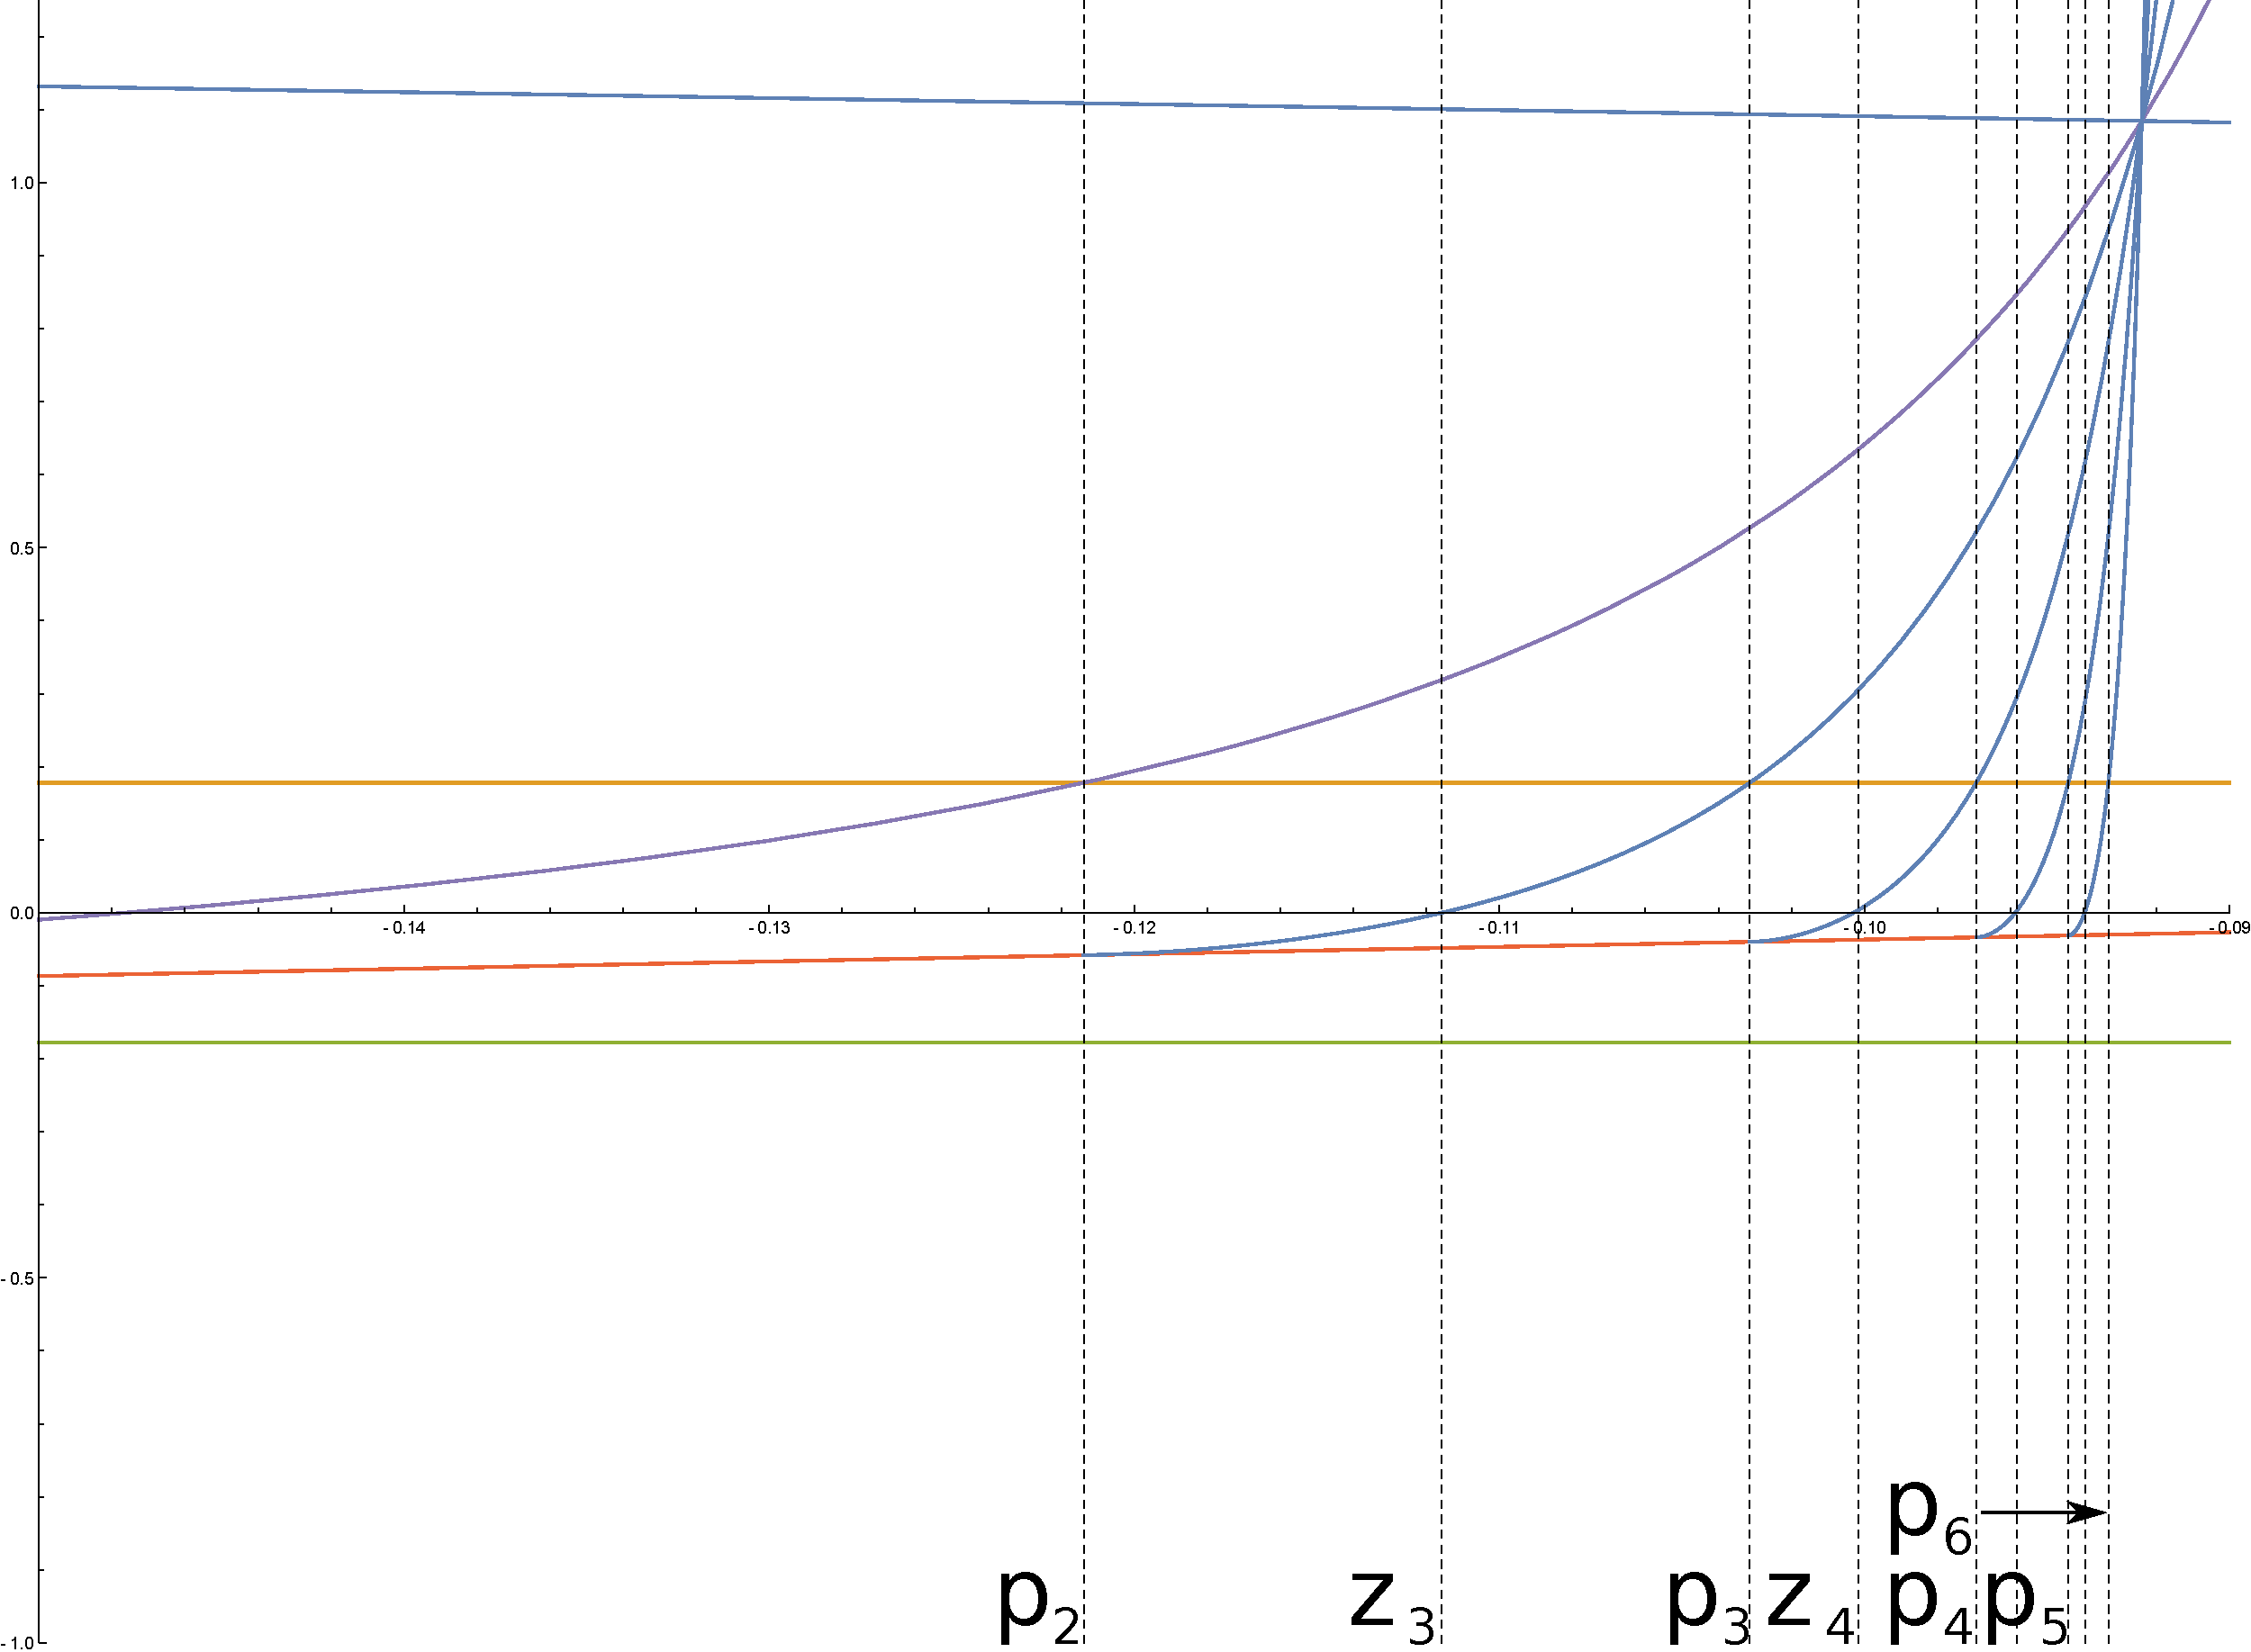
\includegraphics[width=\textwidth]{./img/cplot5H}
% 				\caption{Sixth iterate of $f_c (C)$ added along with the parameter value of its superattracting periodic orbit}
% 				\label{fig:cplot5H}
% 		\end{subfigure}%
% 		~ %add desired spacing between images, e. g. ~, \quad, \qquad, \hfill etc.
% 		  % (or a blank line to force the subfigure onto a new line)
% 		\begin{subfigure}[b]{0.5\textwidth}
% 				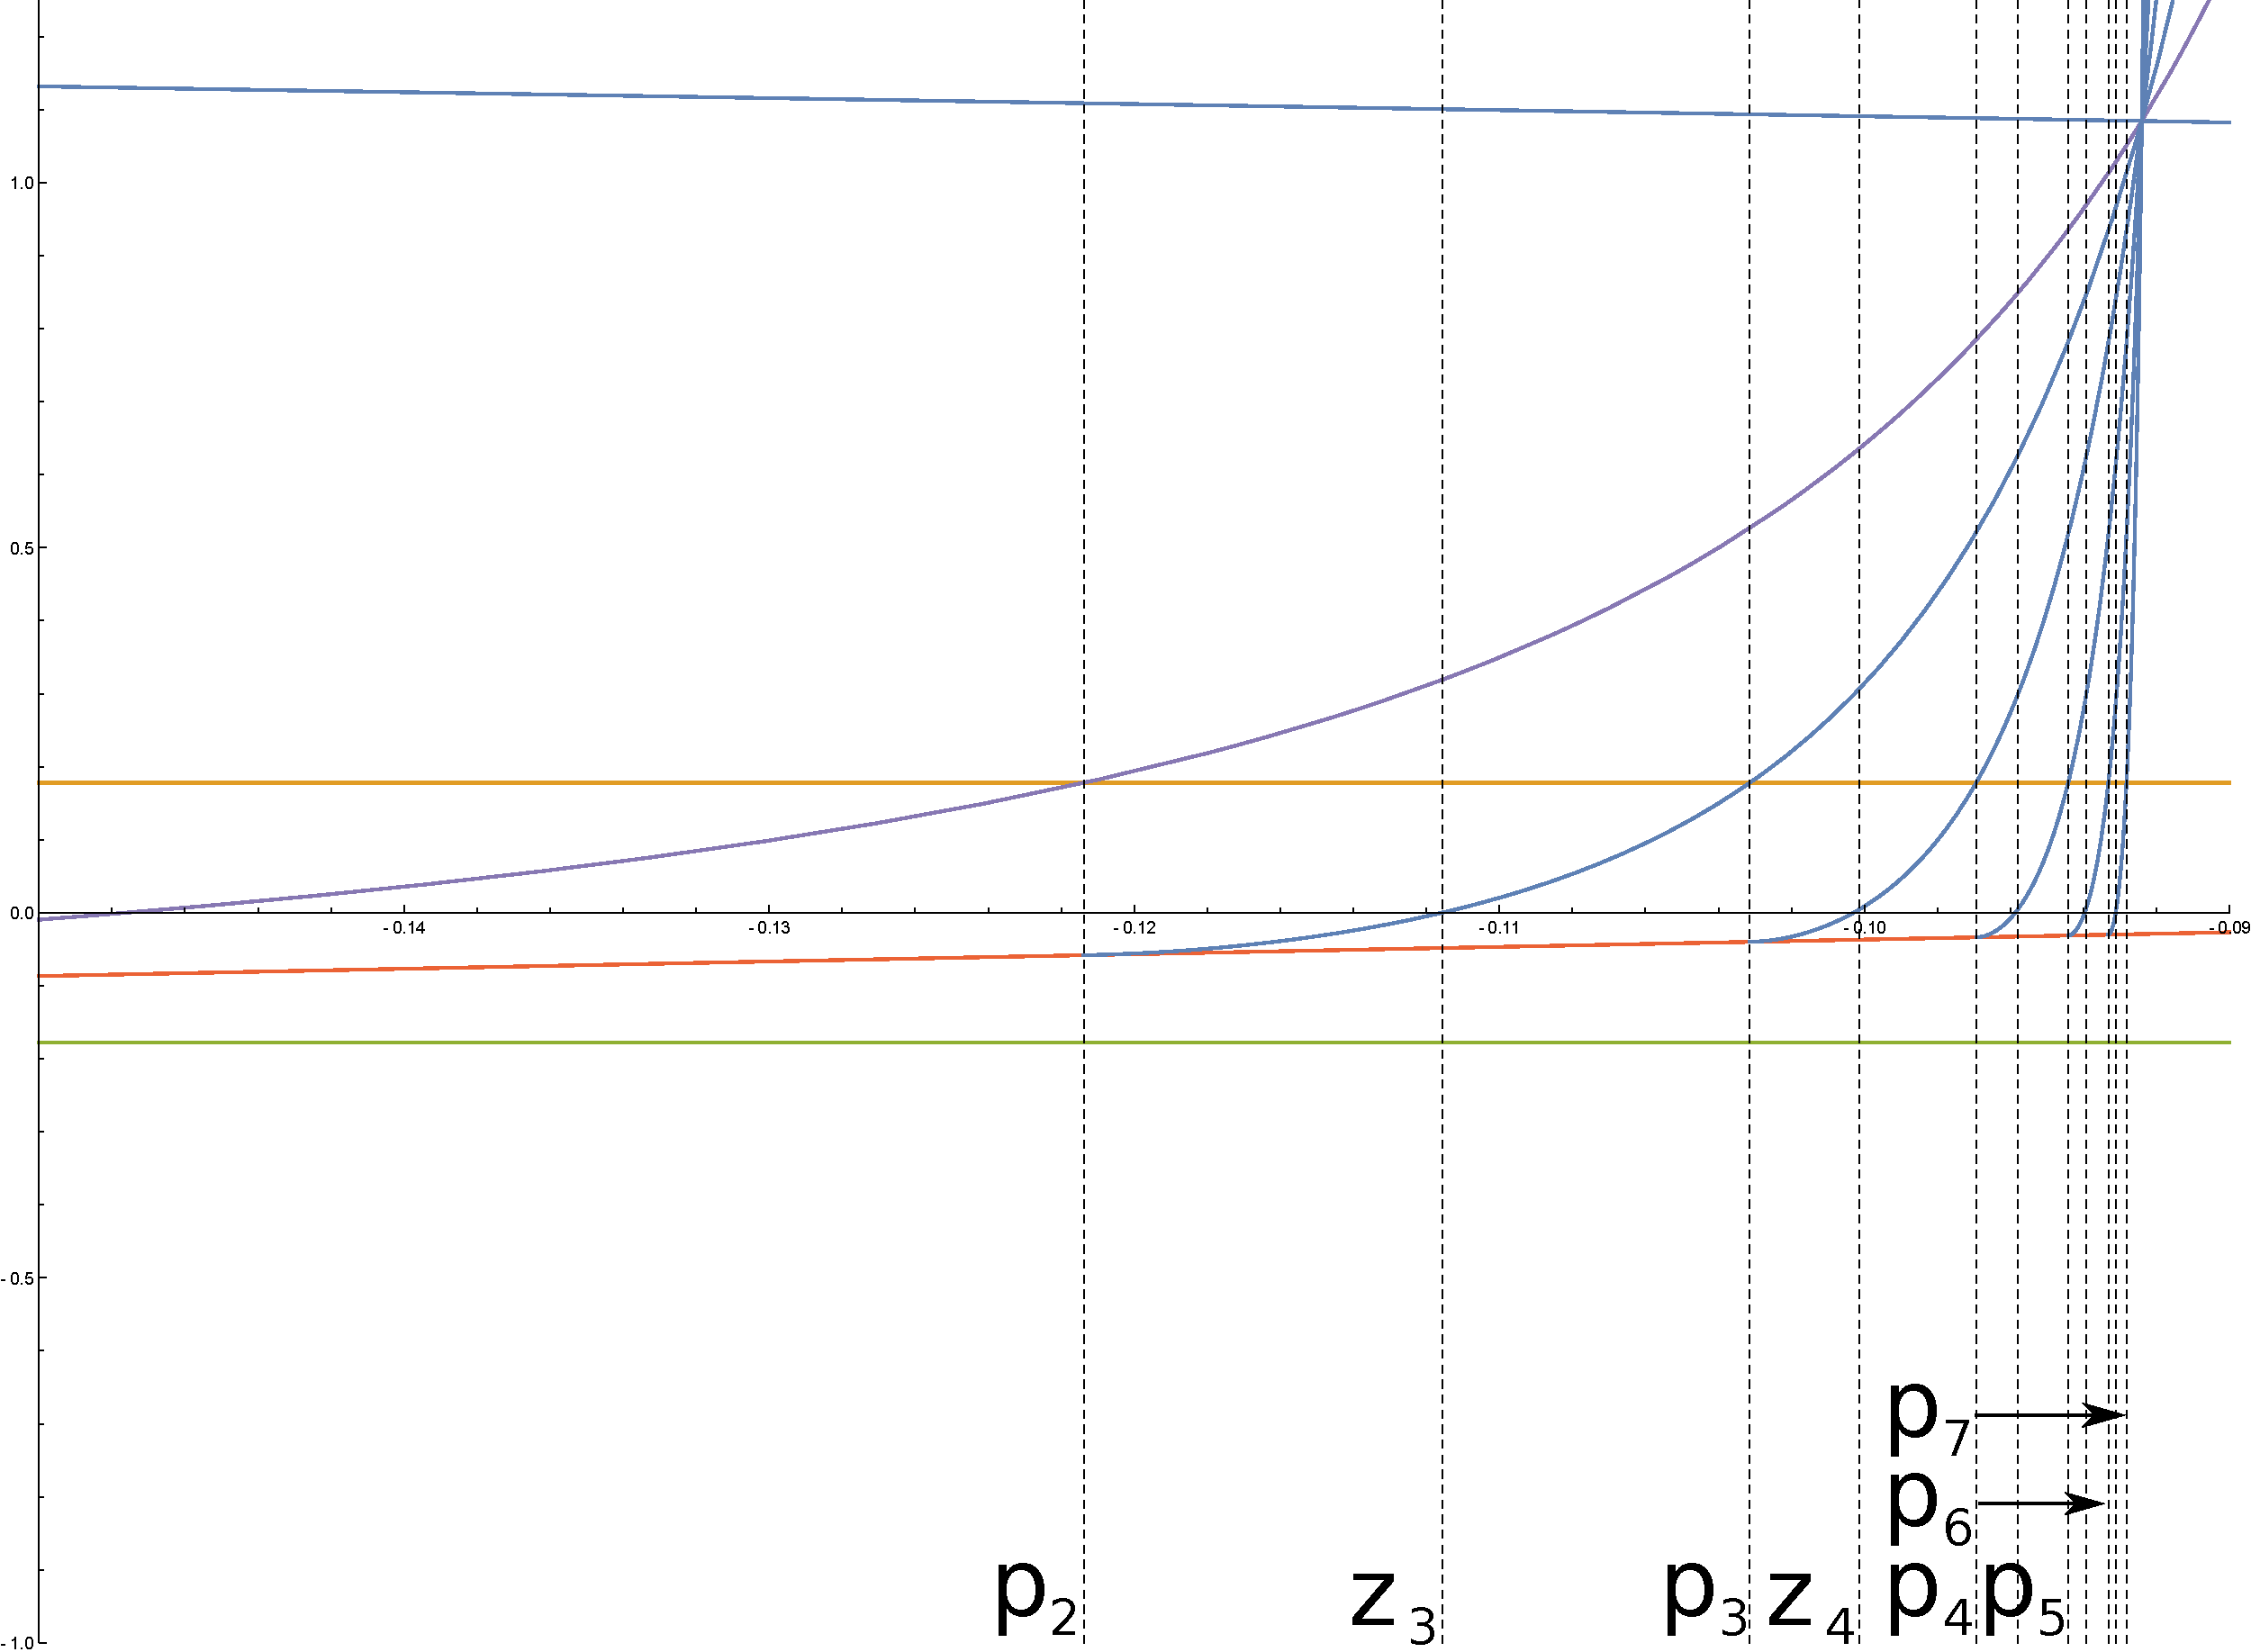
\includegraphics[width=\textwidth]{./img/cplot6H}
% 				\caption{Seventh iterate of $f_c (C)$ added along with the parameter value of its superattracting periodic orbit}
% 				\label{fig:cplot6H}
% 		\end{subfigure}
% 		~ %add desired spacing between images, e. g. ~, \quad, \qquad, \hfill etc.
% 		  % (or a blank line to force the subfigure onto a new line)
% 		\caption{Plots depicting the accumulation of higher order superattracting periodic orbits near $\pr$}\label{fig:iterh}
% \end{figure}

\begin{figure}[ht]
		\centering
		\begin{subfigure}[b]{0.5\textwidth}
				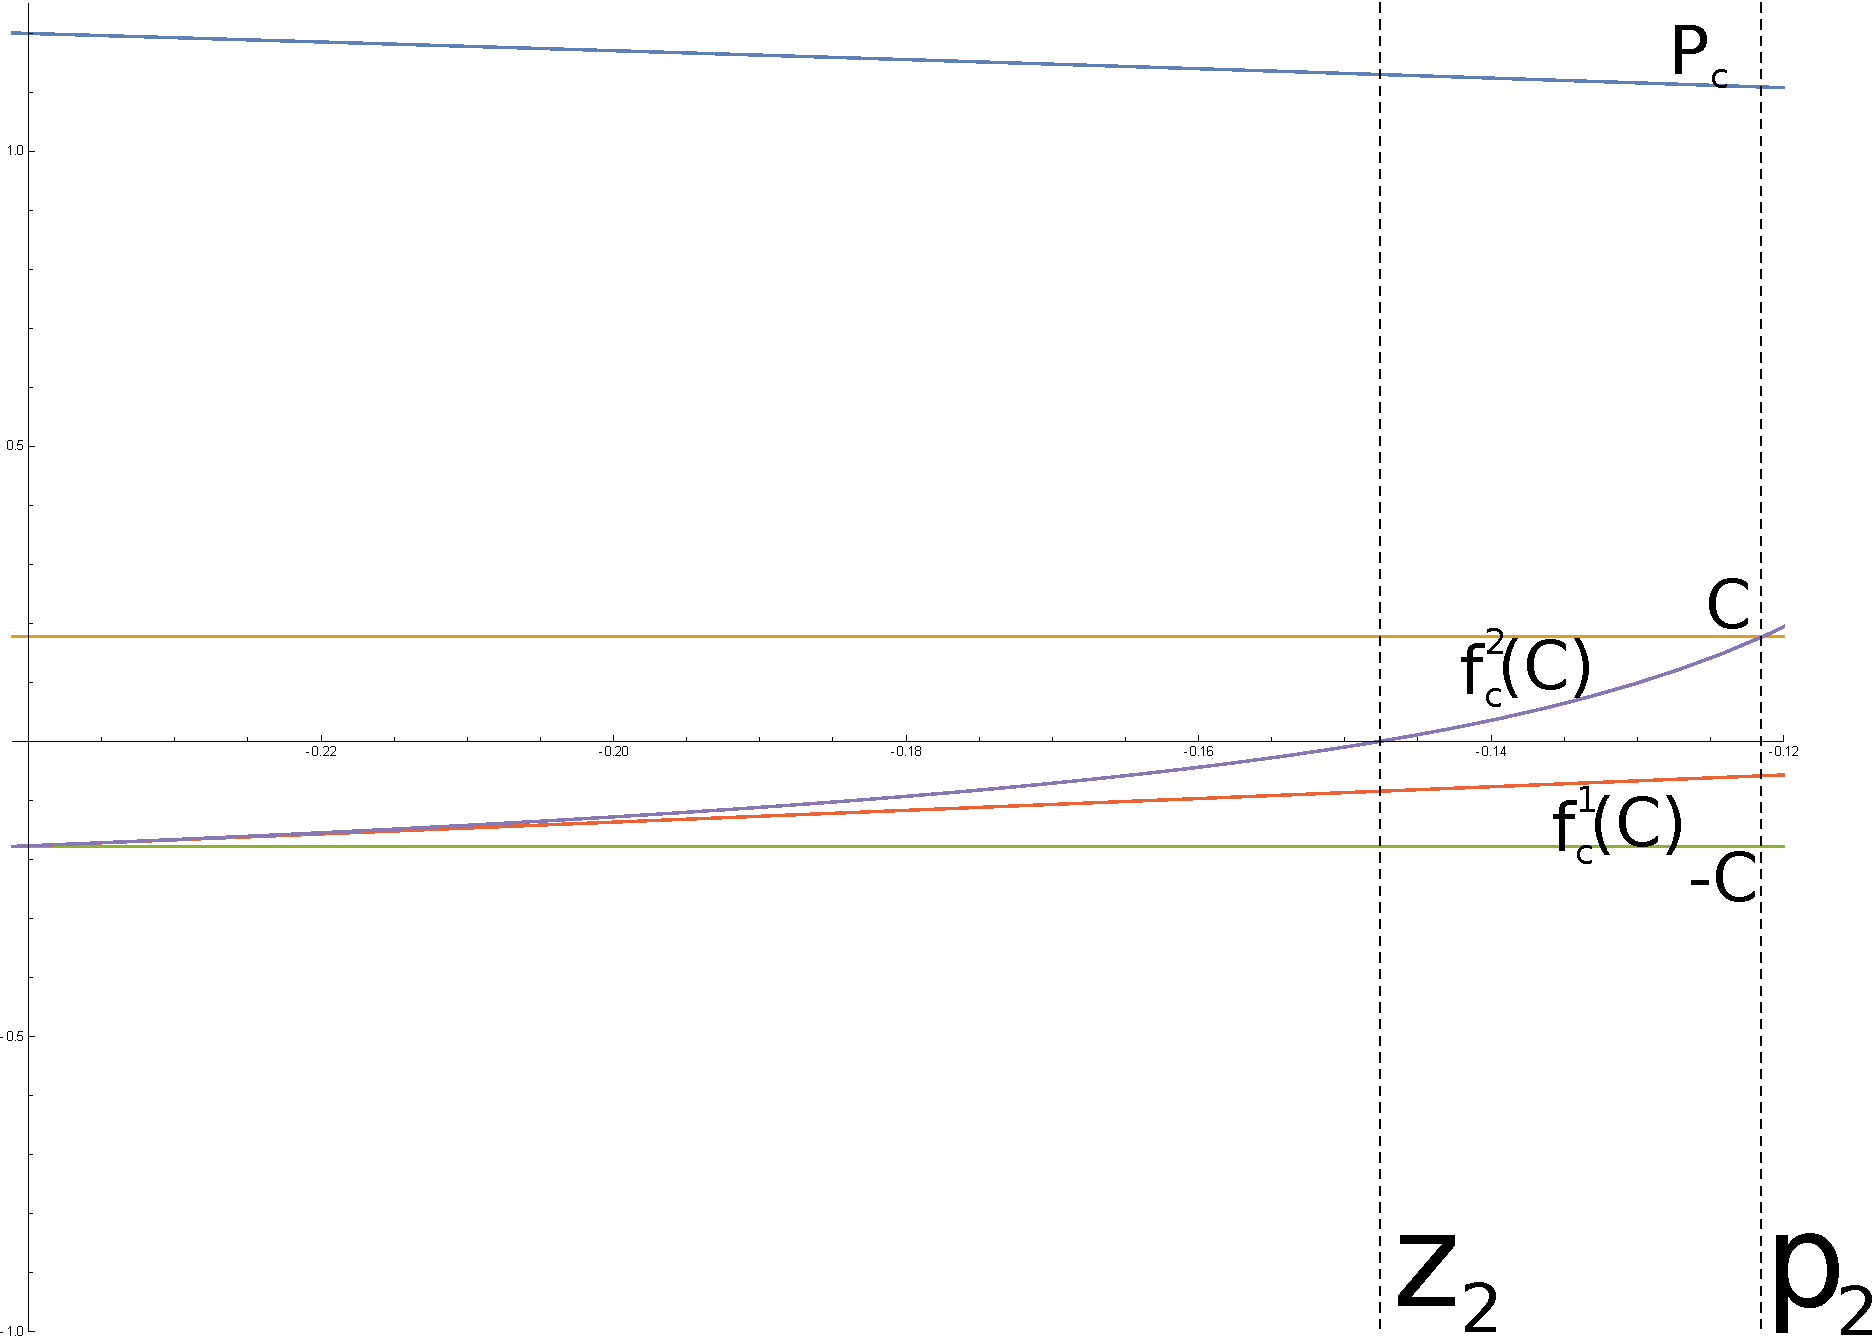
\includegraphics[width=\textwidth]{./img/cplot1S}
				\caption{First two iterates of $f_c (C)$ along with the parameter value of $f^2_c (C)$'s prezero orbit}
				\label{fig:cplot1S}
		\end{subfigure}%
		~ %add desired spacing between images, e. g. ~, \quad, \qquad, \hfill etc.
		  % (or a blank line to force the subfigure onto a new line)
		\begin{subfigure}[b]{0.5\textwidth}
				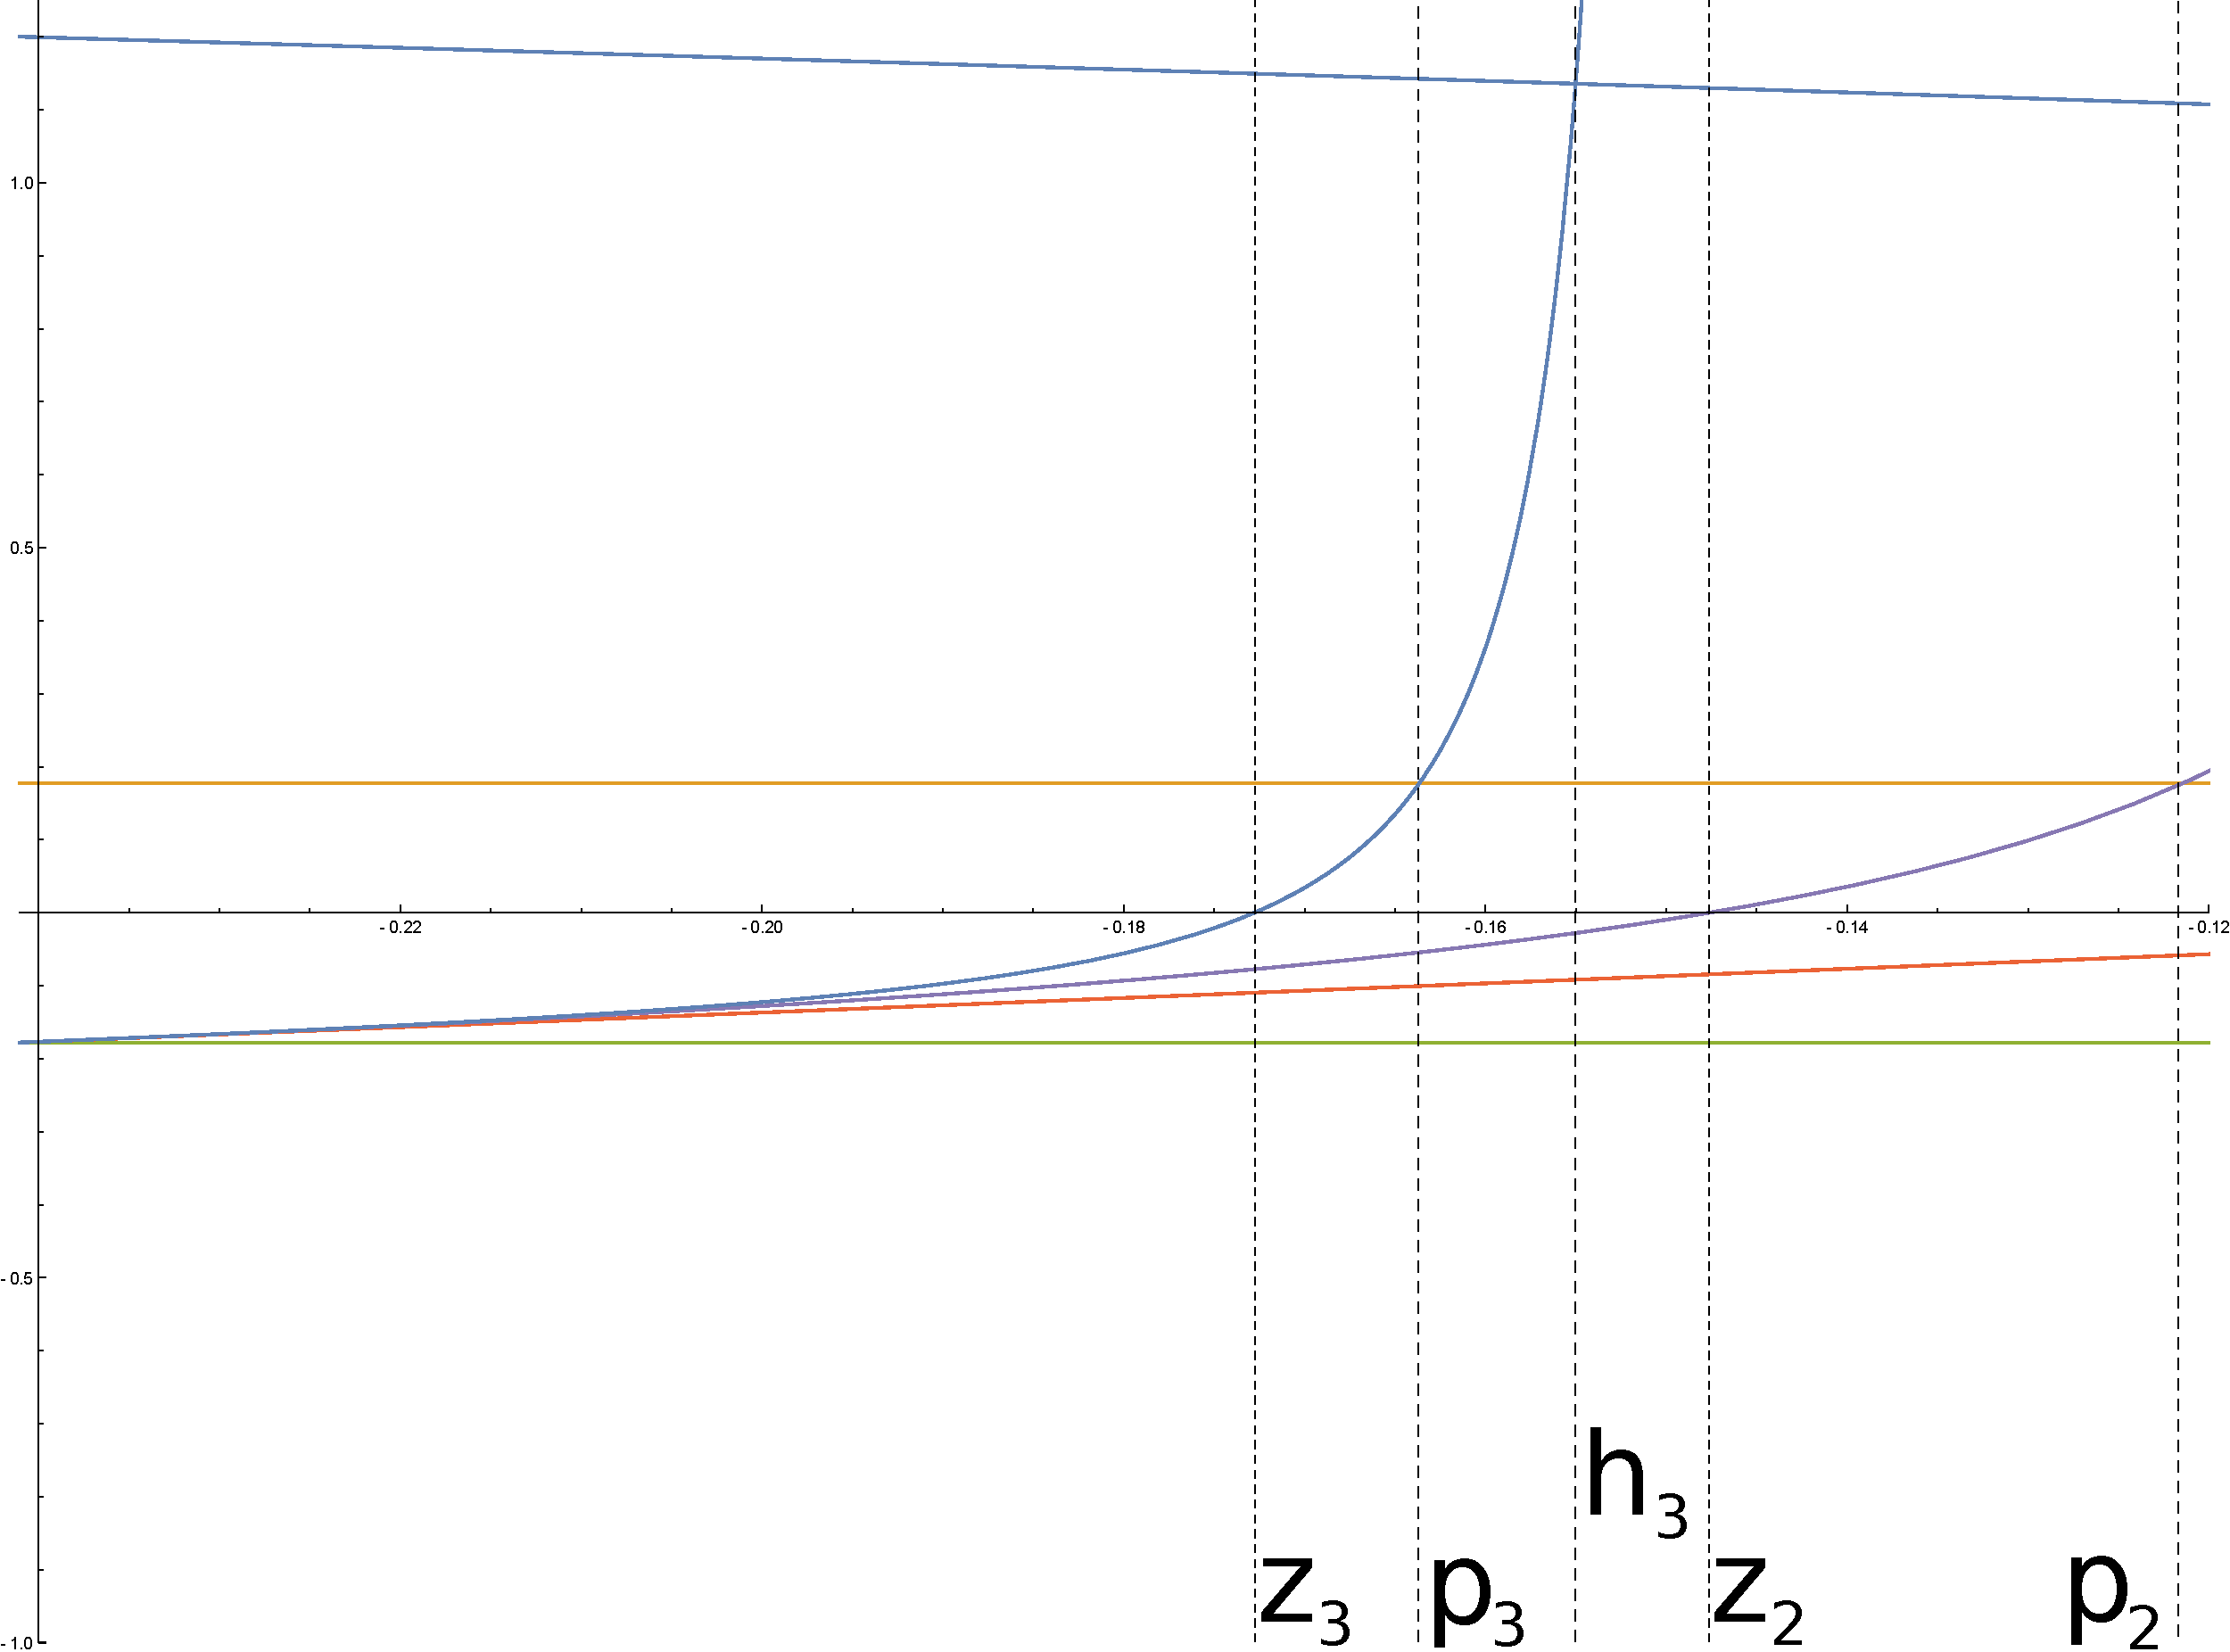
\includegraphics[width=\textwidth]{./img/cplot2S}
				\caption{Third iterate of $f_c (C)$ added along with the parameter value of its prezero orbit}
				\label{fig:cplot2S}
		\end{subfigure}
		\begin{subfigure}[b]{0.5\textwidth}
				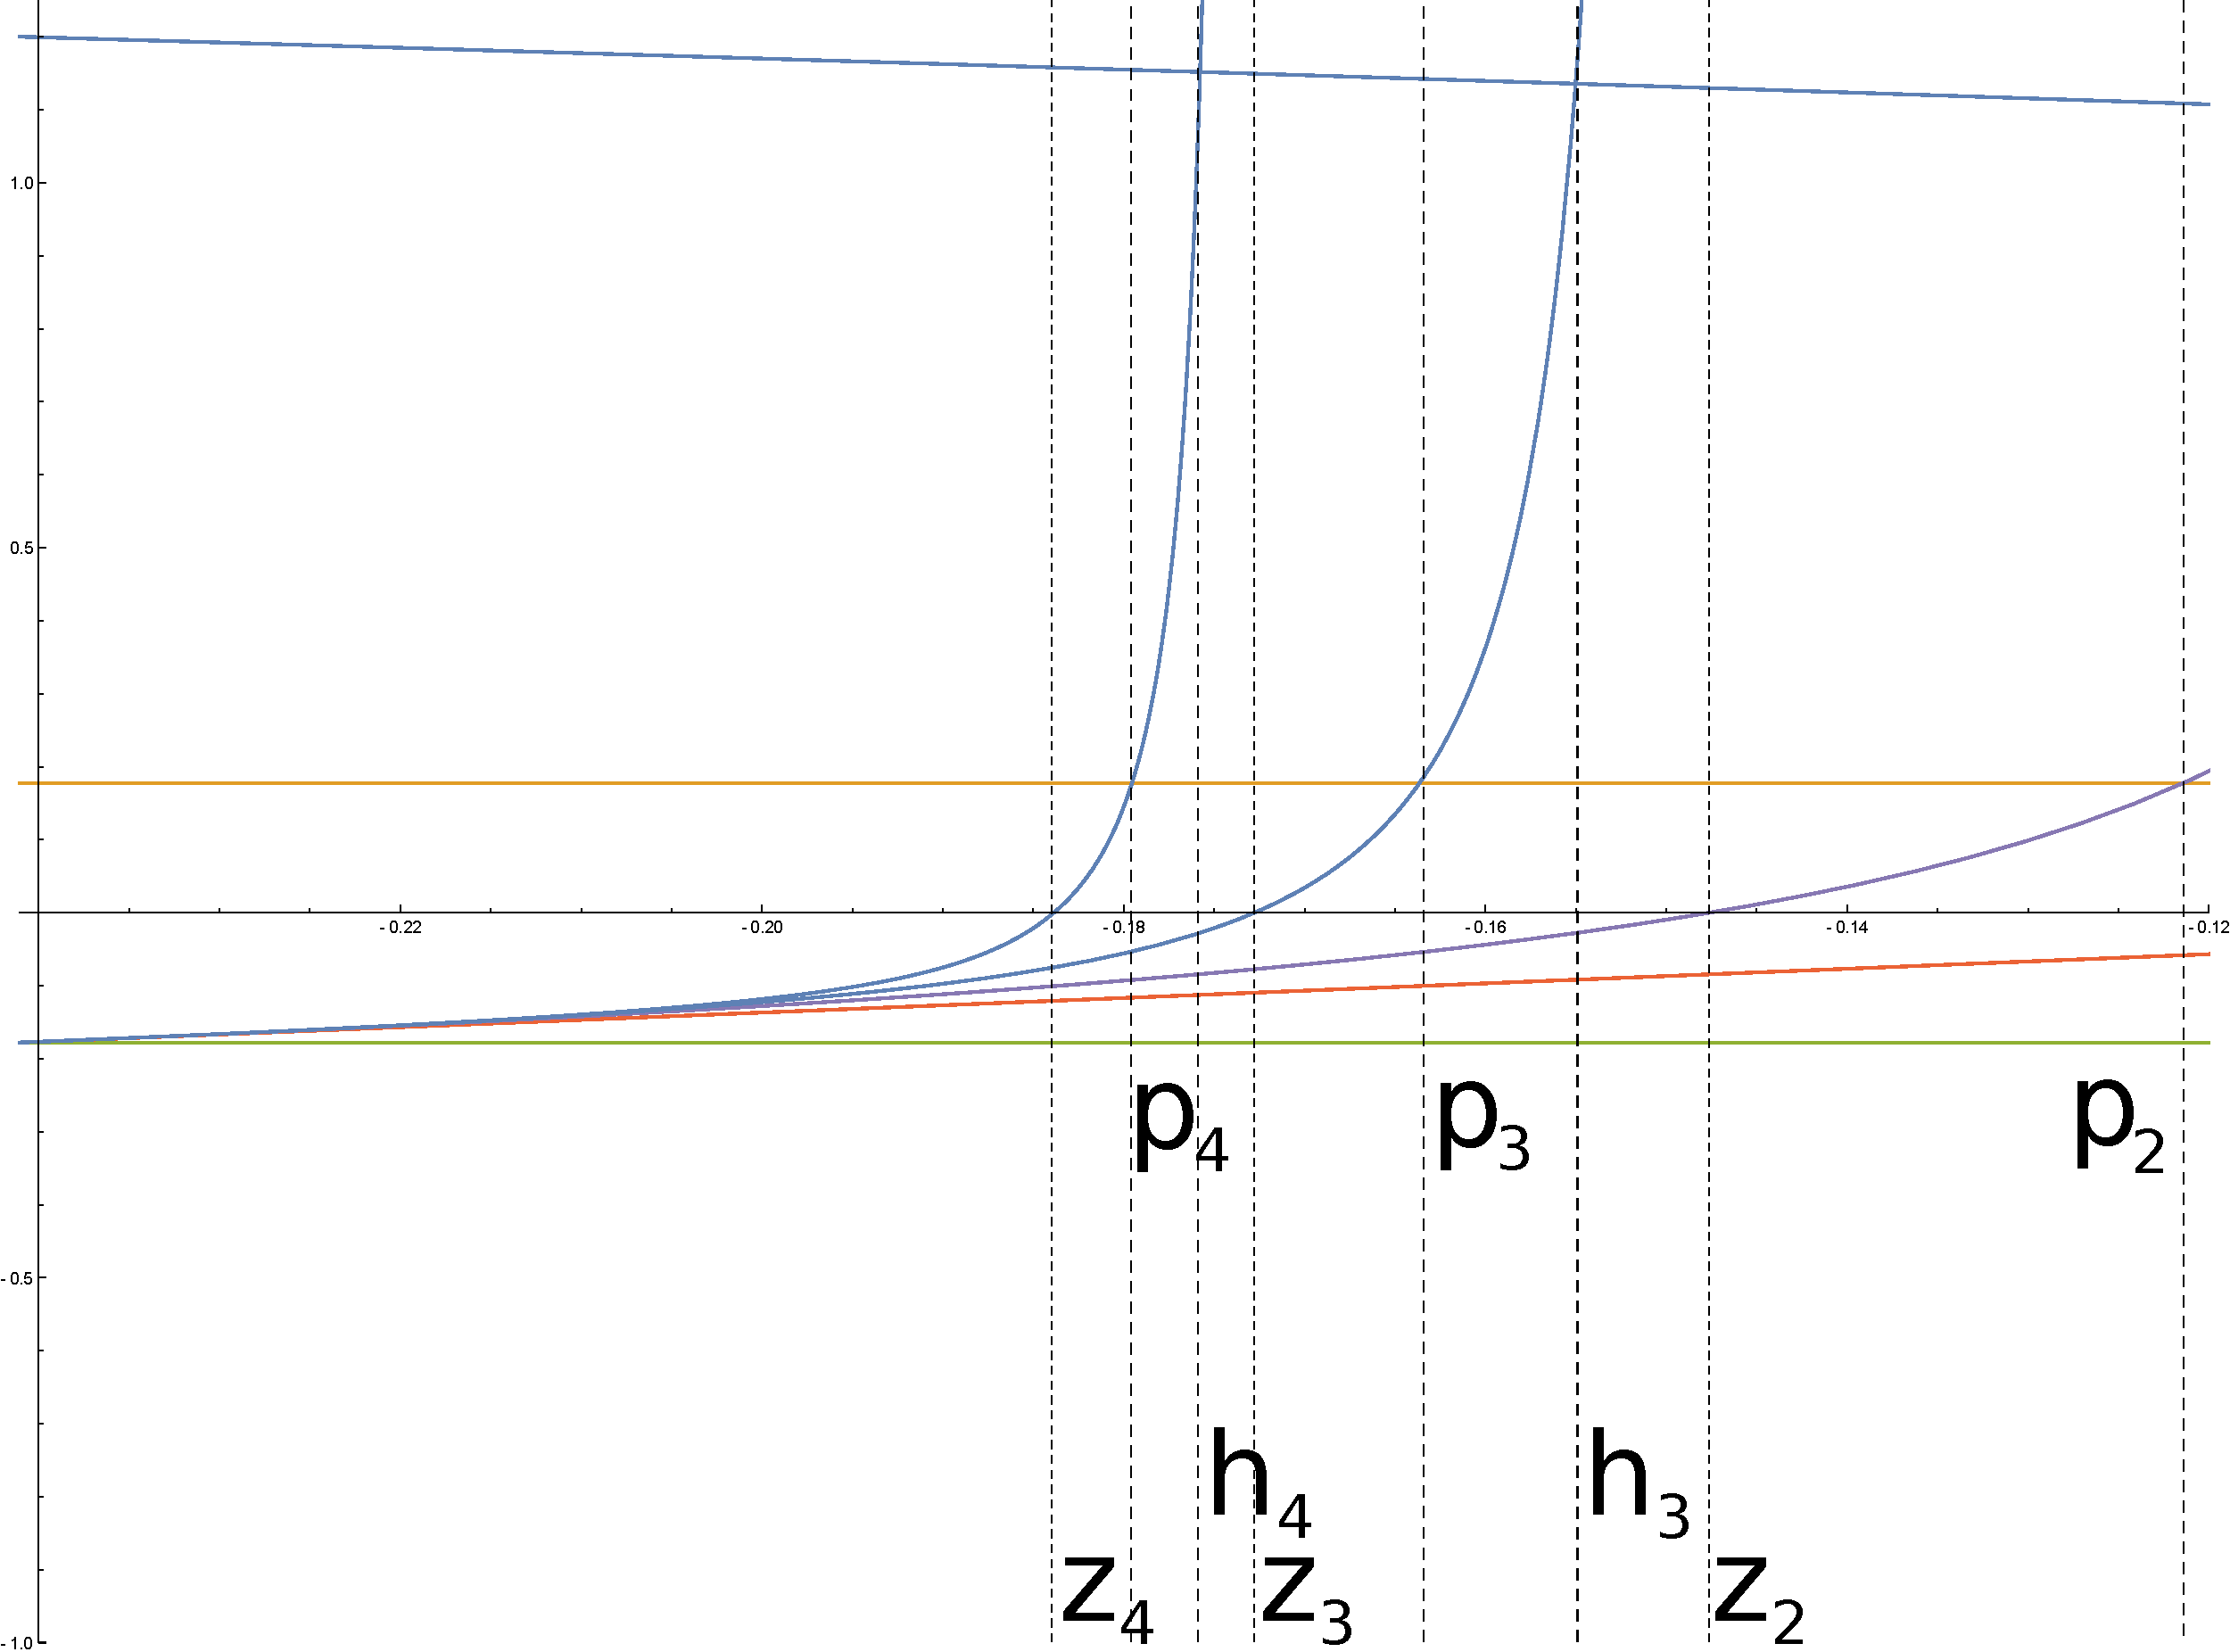
\includegraphics[width=\textwidth]{./img/cplot3S}
				\caption{Fourth iterate of $f_c (C)$ added along with the parameter value of its prezero orbit}
				\label{fig:cplot3S}
		\end{subfigure}%
		~ %add desired spacing between images, e. g. ~, \quad, \qquad, \hfill etc.
		  % (or a blank line to force the subfigure onto a new line)
		\begin{subfigure}[b]{0.5\textwidth}
				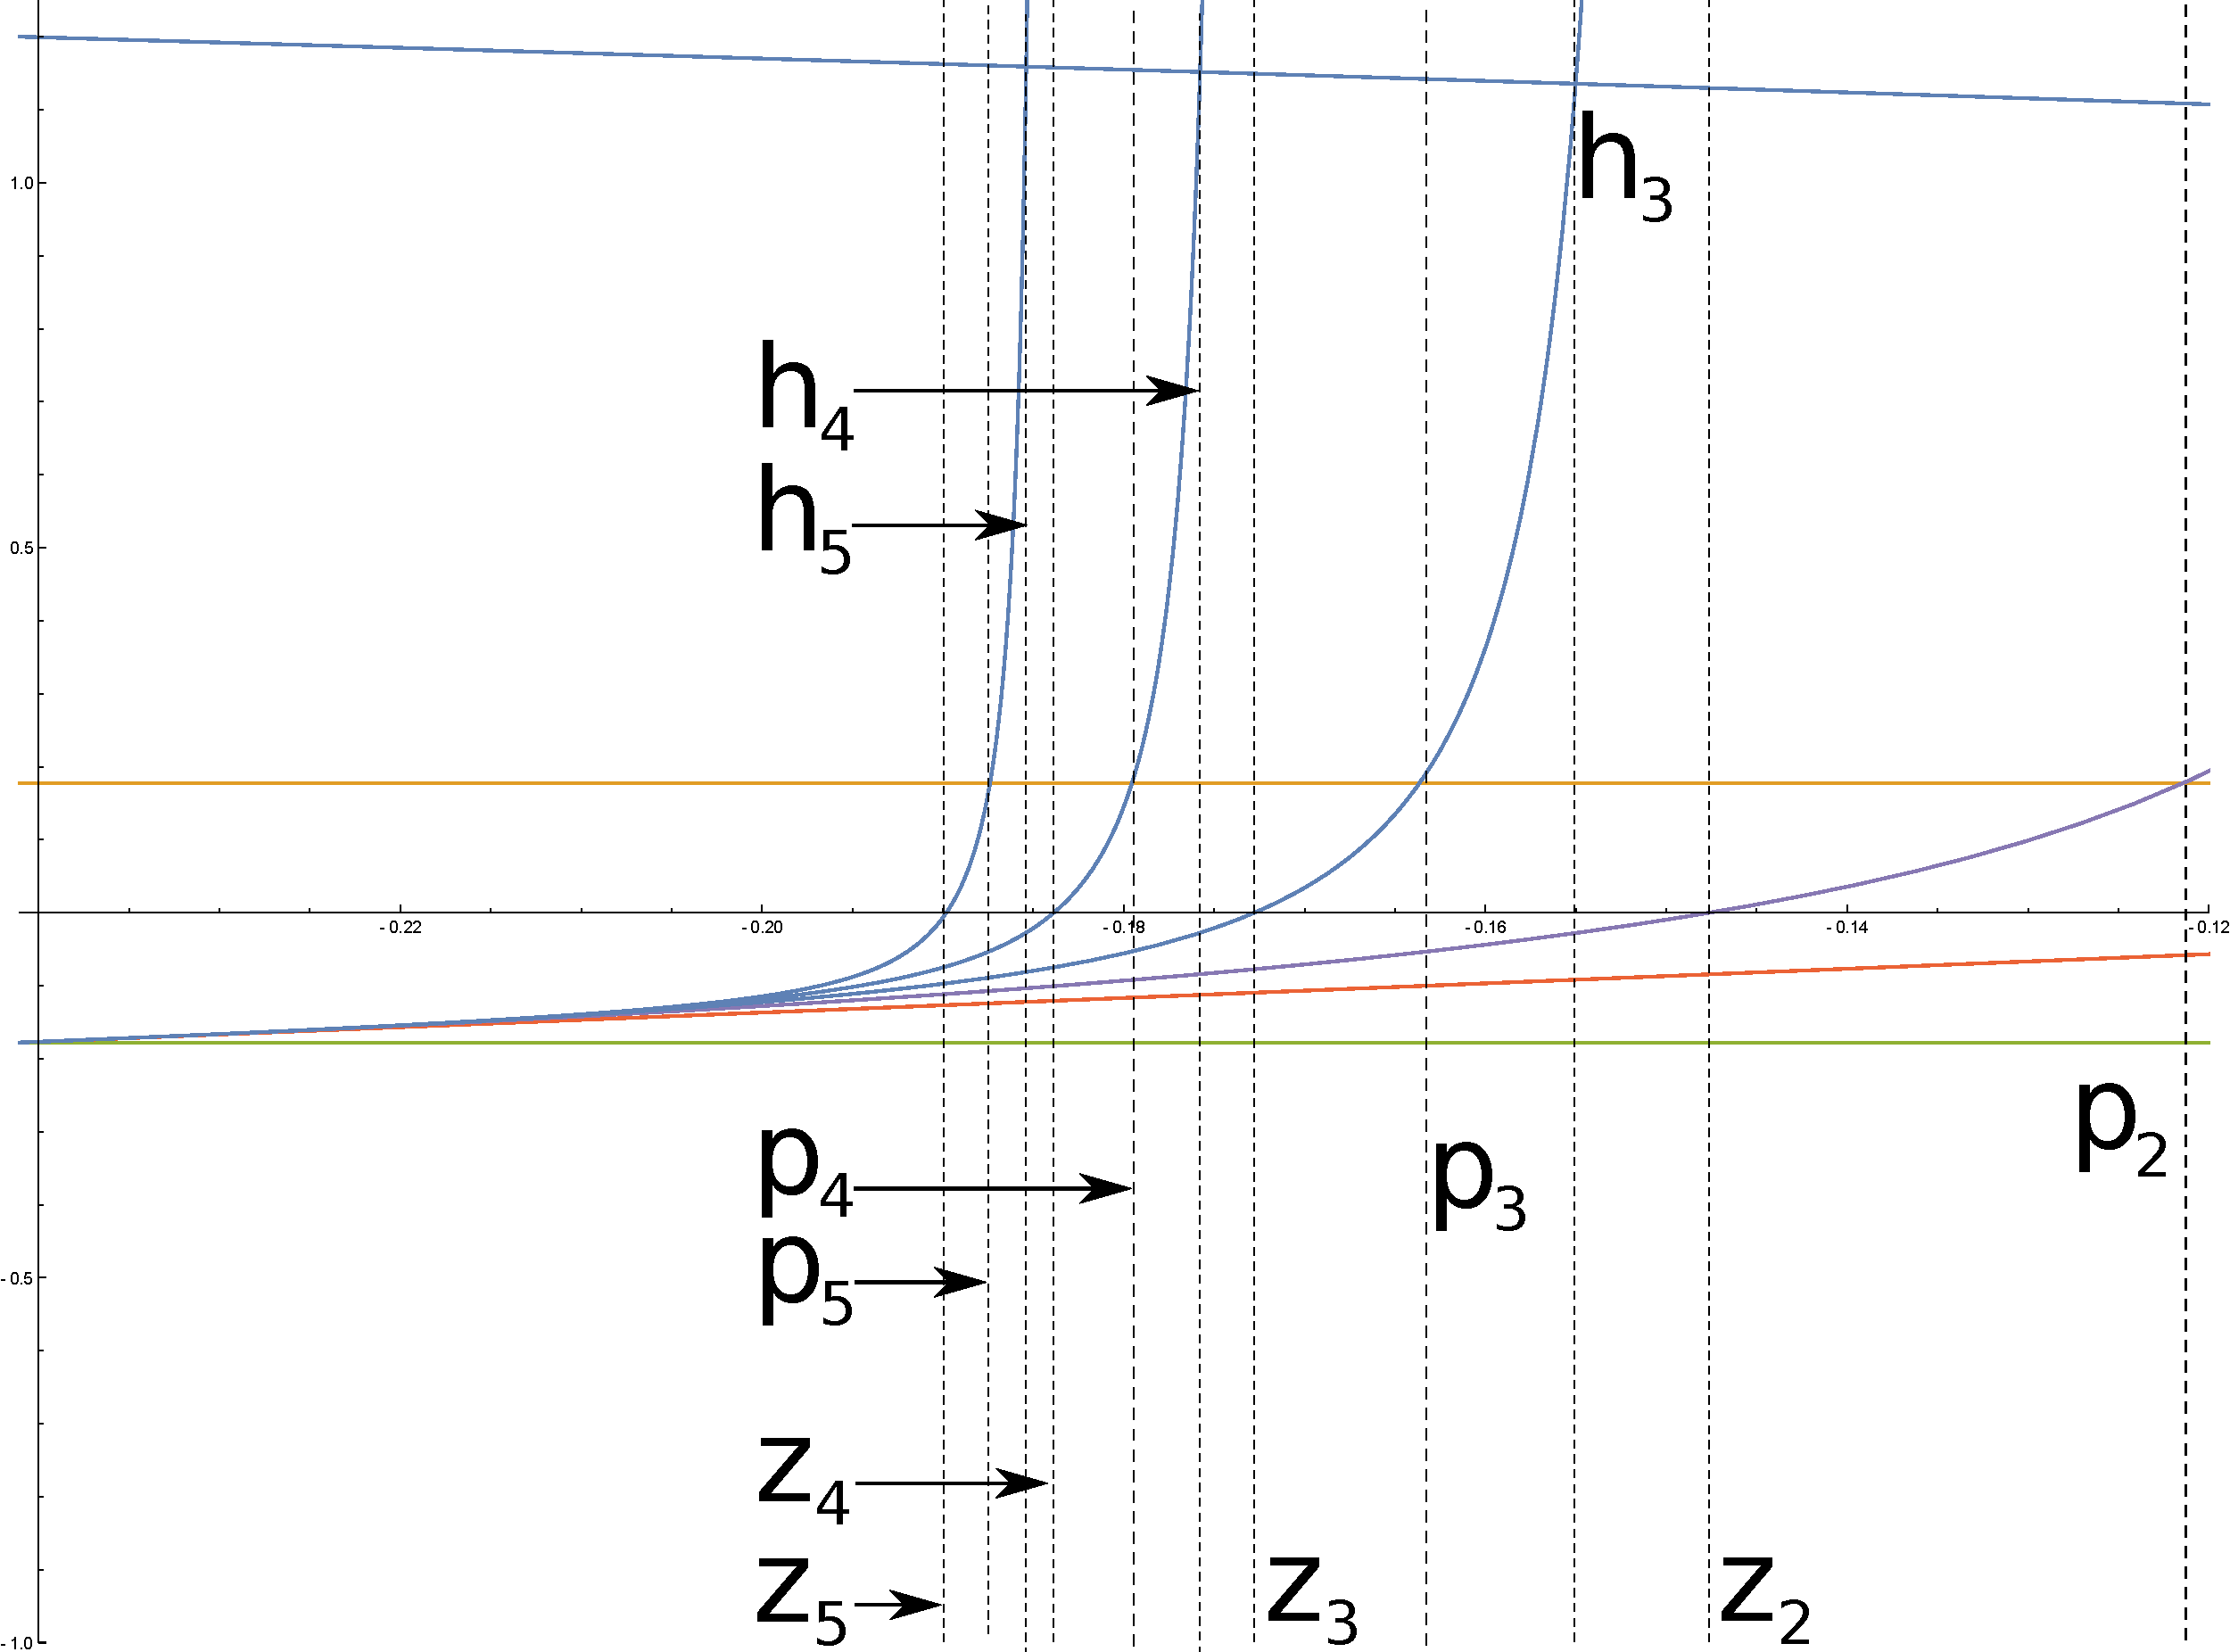
\includegraphics[width=\textwidth]{./img/cplot4S}
				\caption{Fifth iterate of $f_c (C)$ added along with the parameter value of its prezero orbit}
				\label{fig:cplot4S}
		\end{subfigure}
		\begin{subfigure}[b]{0.5\textwidth}
				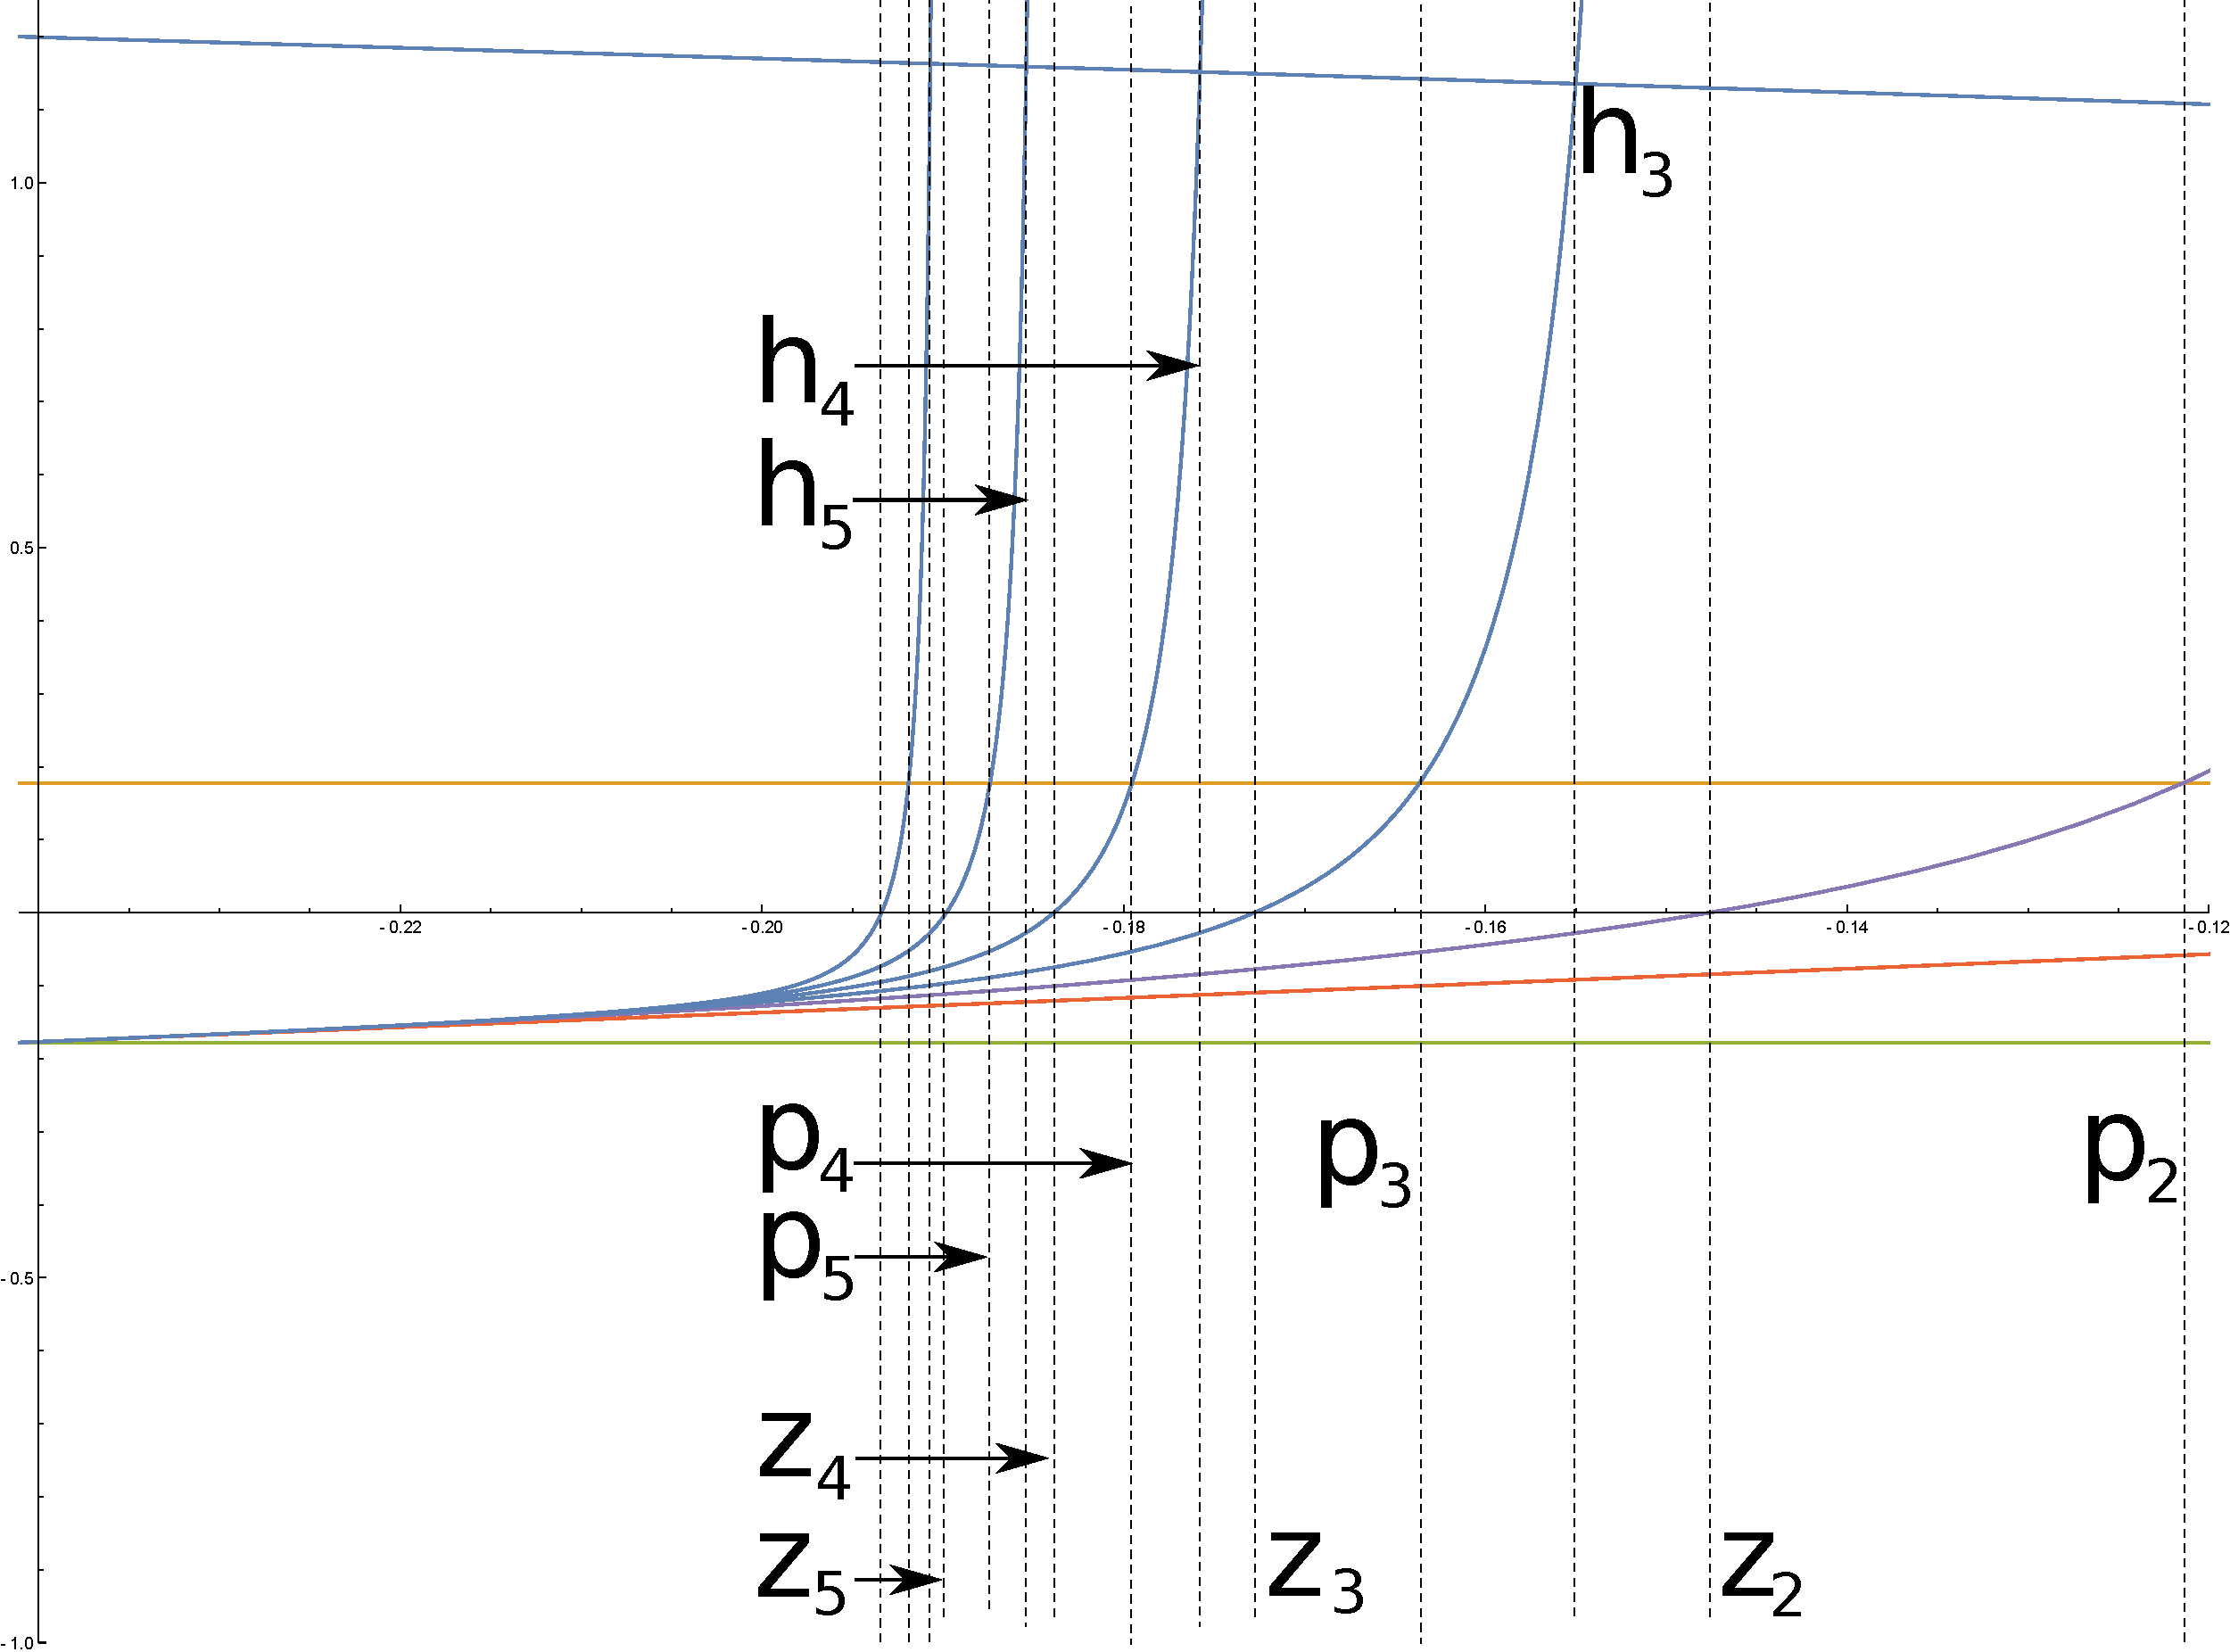
\includegraphics[width=\textwidth]{./img/cplot5S}
				\caption{Sixth iterate of $f_c (C)$ added along with the parameter value of its prezero orbit}
				\label{fig:cplot5S}
		\end{subfigure}%
		~ %add desired spacing between images, e. g. ~, \quad, \qquad, \hfill etc.
		  % (or a blank line to force the subfigure onto a new line)
		\begin{subfigure}[b]{0.5\textwidth}
				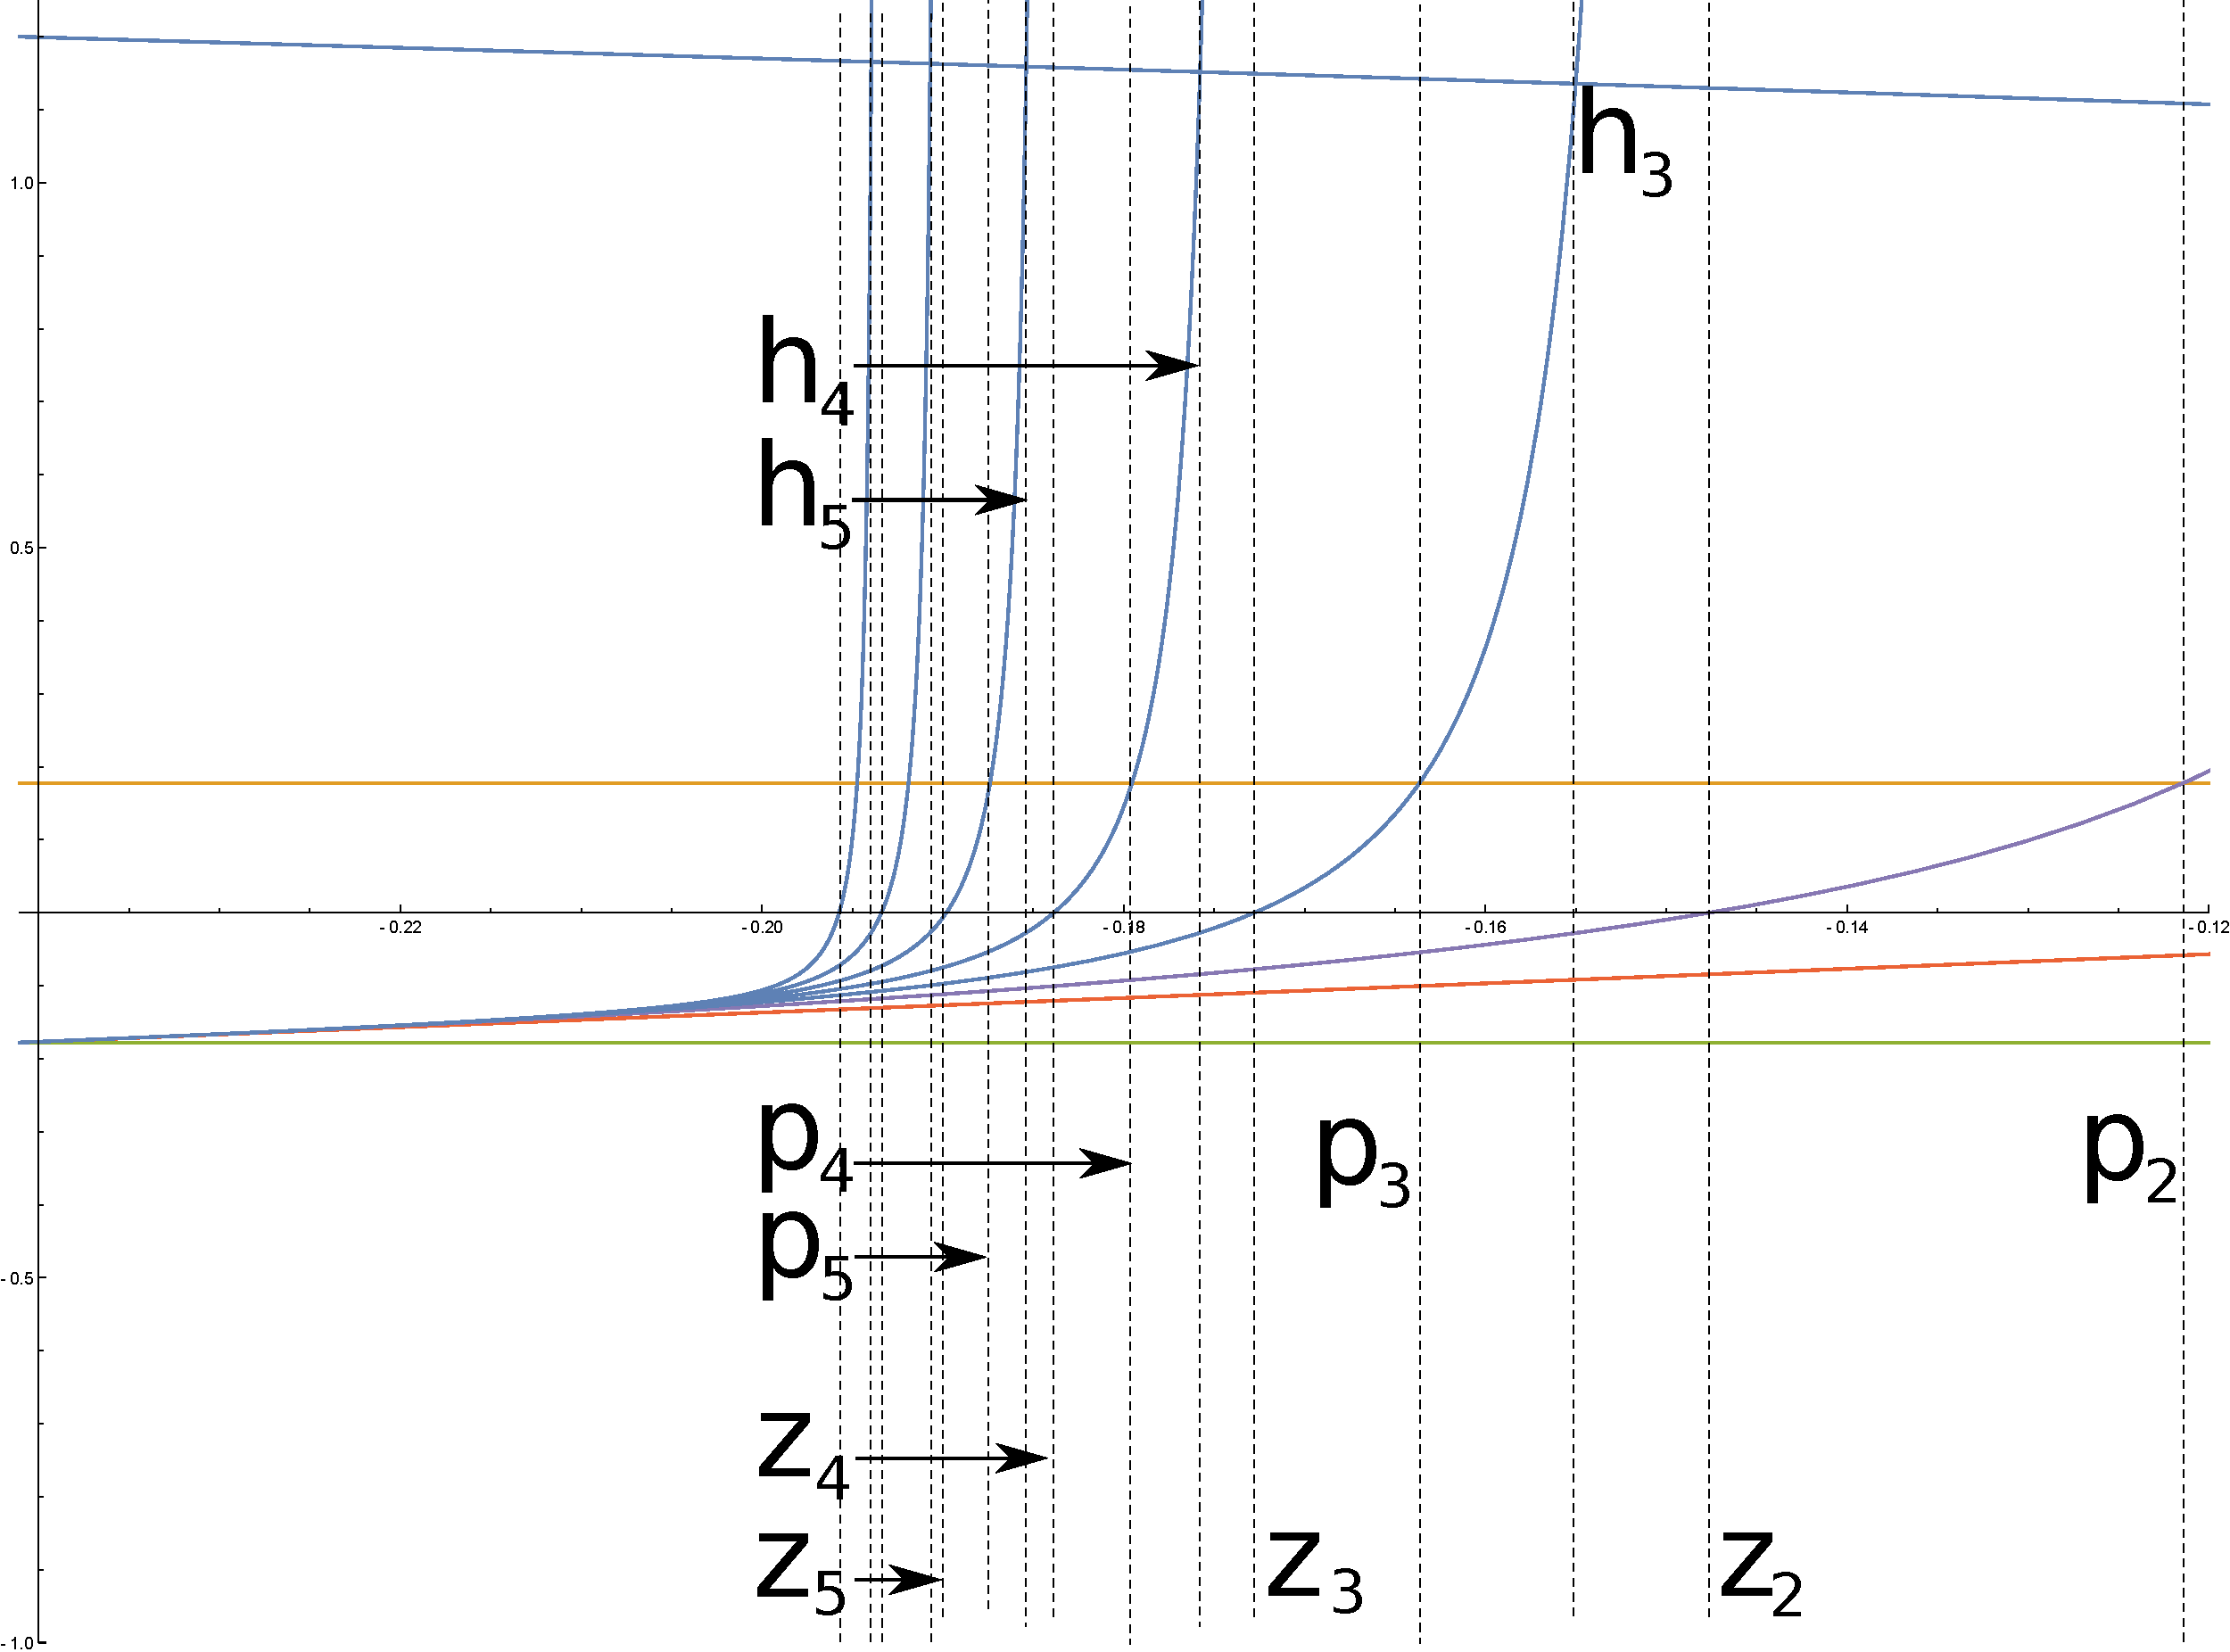
\includegraphics[width=\textwidth]{./img/cplot6S}
				\caption{Seventh iterate of $f_c (C)$ added along with the parameter value of its prezero orbit}
				\label{fig:cplot6S}
		\end{subfigure}
		~ %add desired spacing between images, e. g. ~, \quad, \qquad, \hfill etc.
		  % (or a blank line to force the subfigure onto a new line)
		\caption{Plots of various iterates of $f_c (C)$ as a function of $c$ depicting the accumulation of prezero, periodic, and prefixed parameter values as we approach $s_1^l$ from the right. Note that for $n > 4$ the $z_n$ and $h_n$ values are marked but not labeled. Also observe that each $f^i_c (C)$ is only plotted on the interval $ (p_{1}^{-C}, z_{i-1})$ in order to highlight specific behaviors}\label{fig:iterh2}
\end{figure}
\FloatBarrier